\documentclass[12pt]{article}
\usepackage{graphicx}
\usepackage[margin=1.0in]{geometry}   % sets all margins to 1in, can be changed
\usepackage{moreverb}                 % for verbatimtabinput -- LaTeX environment
\usepackage{rotating}
\usepackage{url}     
\usepackage{hyperref}
\usepackage{multirow}
\usepackage{amssymb}                  % for many mathematical symbols
\usepackage[pdftex]{lscape}           % for landscaped tables
\usepackage{longtable}
\usepackage[dvipsnames]{xcolor}
\usepackage[spanish]{babel}
\usepackage[utf8]{inputenc}

\title{Un primer estudio estad\'istico de la Certificaci\'on en la UACM}
\author{Carlos E. Martínez-Rodríguez\thanks{Departamento de Estadística, Universidad Autónoma de la Ciudad de México (UACM). Correo electrónico: carlos.martinez@uacm.edu.mx}}
\date{27 de noviembre de 2022}

\begin{document}
\maketitle
%\tableofcontents

\section{Introducci\'on y antecedentes}



\begin{figure}
\centering
\includegraphics[scale=0.45]{Graficas/BarPlotPlantelCal.pdf}
\caption{Certificaciones por Planteles}
\label{Fig.Cert.Plantel-Cal}
\end{figure}

La Universidad Aut\'onoma de la Ciudad de M\'exico fue creada el 26 de abril de 2001 por el gobierno del Distrito federal a trav\'es del \href{https://www.uacm.edu.mx/Portals/0/adam/Content/hfXbhKHHXE2k2Y8j2fG9UQ/Text/DCUACM.pdf}{decreto de creaci\'on} publicado en la Gaceta Oficial del Distrito Federal por el Jefe de gobierno de la Ciudad de M\'exico, m\'as adelante, el 16 de diciembre de 2004 la Asamblea Legislativa del Distrito Federal, III Legislatura, aprob\'o la \href{https://www.uacm.edu.mx/Portals/0/ley_uacm092011.pdf}{Ley de la Universidad Aut\'onoma de la Ciudad de M\'exico} misma que fue publicada el 5 de enero de 2005.


\begin{figure}
\centering
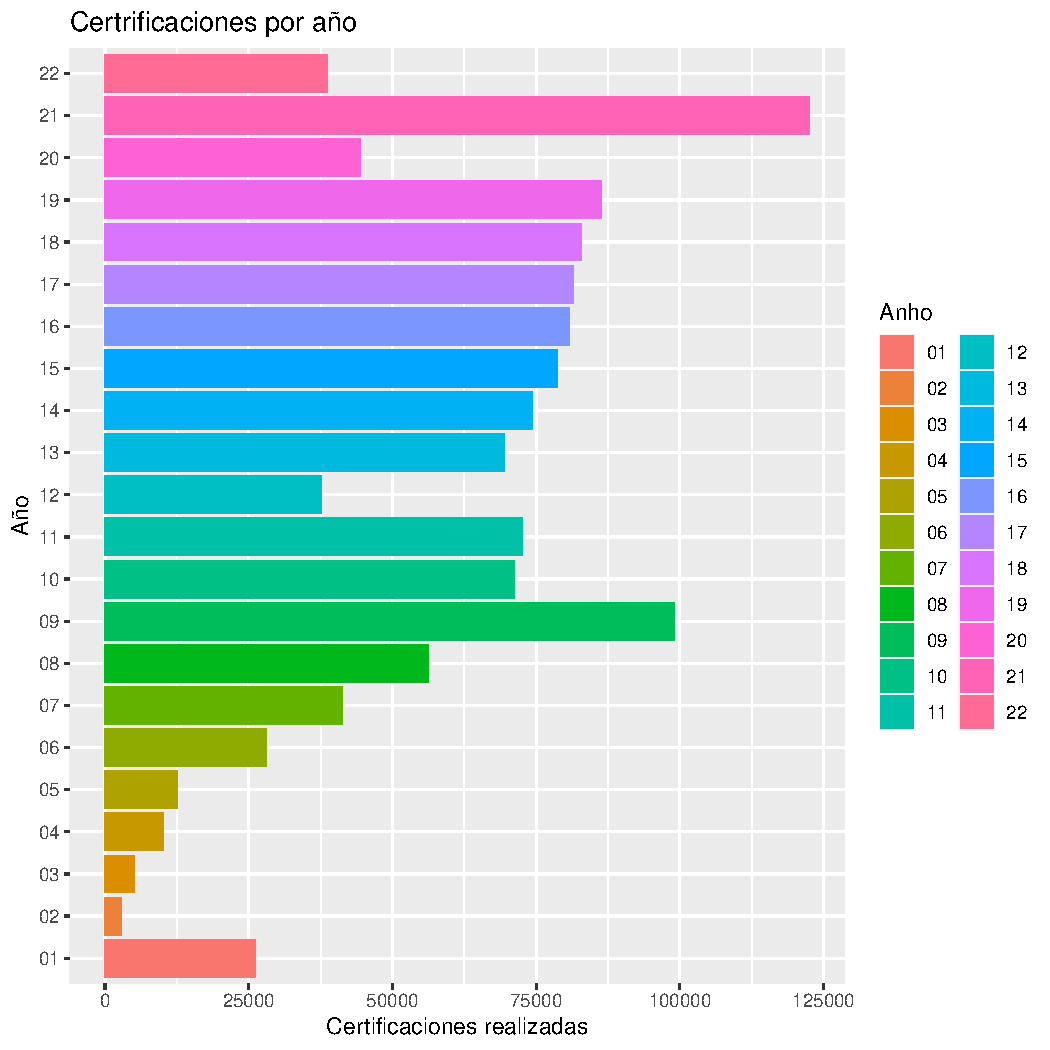
\includegraphics[scale=0.45]{Graficas/ggplotBarplotAnho.pdf}
\caption{Certificaciones por A\~no}
\label{Fig.Cert.Anho}
\end{figure}


El \href{https://drive.google.com/file/d/0B6AEksrqo4h1M2Q5OWVhOGEtODNlNy00M2M2LThkNTctZjE0ZjA4ZGJlZWZj/view?resourcekey=0-9eA5mzOWlPqKF8MTeYH9Iw}{proyecto educativo de la UACM} enuncia que una de las acciones educativas en funci\'on del aprendizaje del estudiante, es procurar que los planes de estudio permitan trayectorias flexibles y que los programas de estudio sean en todo coherentes con sus prop\'ositos formativos, que las formas de evaluaci\'on y presentaci\'on de resultados sean \'utiles a las y los estudiantes, aportando orientaciones  para superar sus dificultades y permitir avanzar en el logro de sus metas de formaci\'on universitaria.


\begin{figure}
\centering
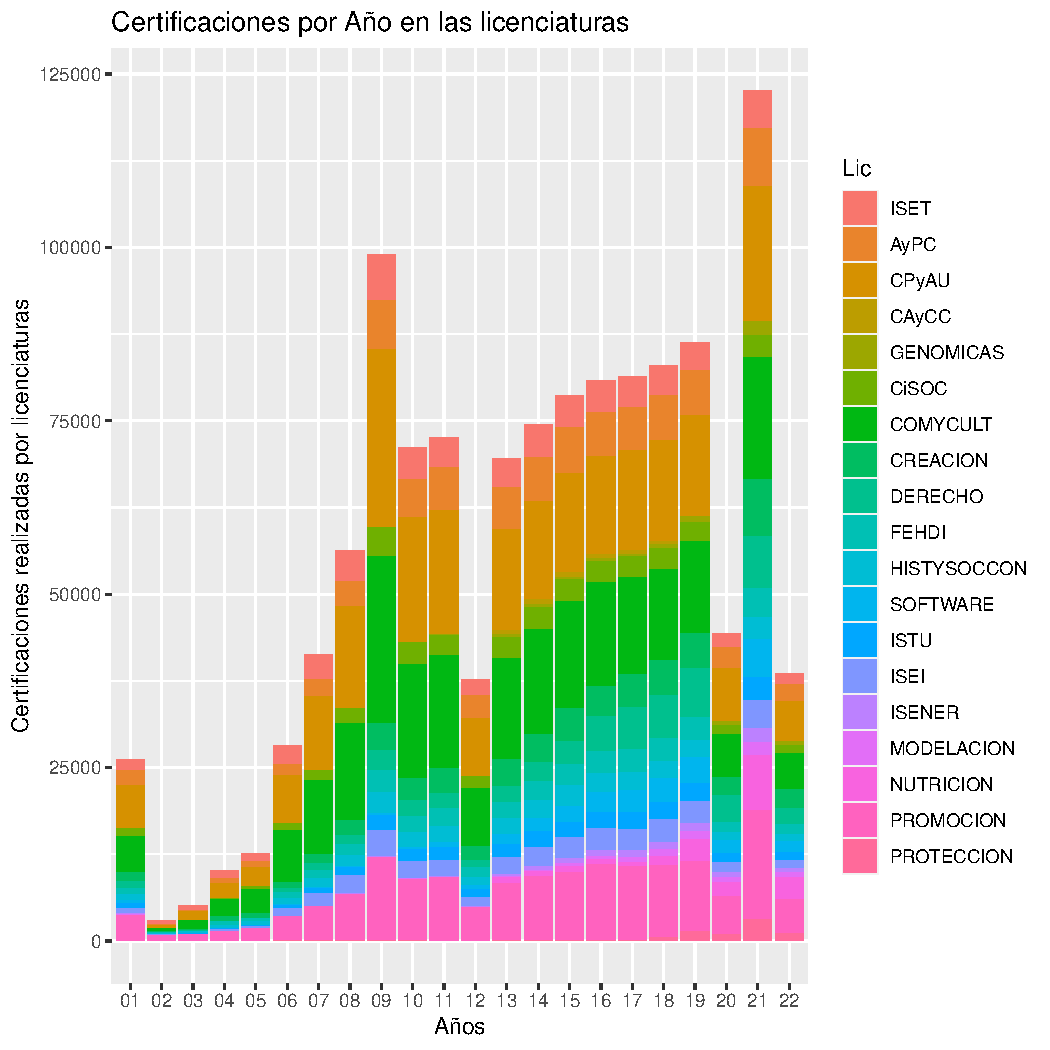
\includegraphics[scale=0.45]{Graficas/ggplotBarplotAnhoLic.pdf}
\caption{Certificaciones por A\~no por licenciatura}
\label{Fig.Cert.Anho-Lic}
\end{figure}




\textit{En la UACM la evaluaci\'on para certificaci\'on tiene la finalidad de dar fe de que el estudiante posee los conocimientos que el certificado ampara. En este sentido se trata de un procedimiento con car\'acter jur\'adico-administrativo, separado de los procesos de ense\~nanza y aprendizaje y las evaluaciones formativas que les son inherentes} \cite{ProyectoEducativo}, continua mencionando que el separar los procesos de ense\~nanza y aprendizaje del de certificaci\'on permite que las y los estudiantes centren su atenci\'on en aprender,  valorando sus propios procesos as\'i como los conocimientos construidos sin la presi\'on de un \'unico momento para certificarlos. Lo anterior permite que las y los estudiantes se puedan registrar y presentarse en cualquiera de las materias que cubre la oferta acad\'emica sin importar d\'onde, o c\'omo los obtuvieron. 

\begin{figure}
\centering
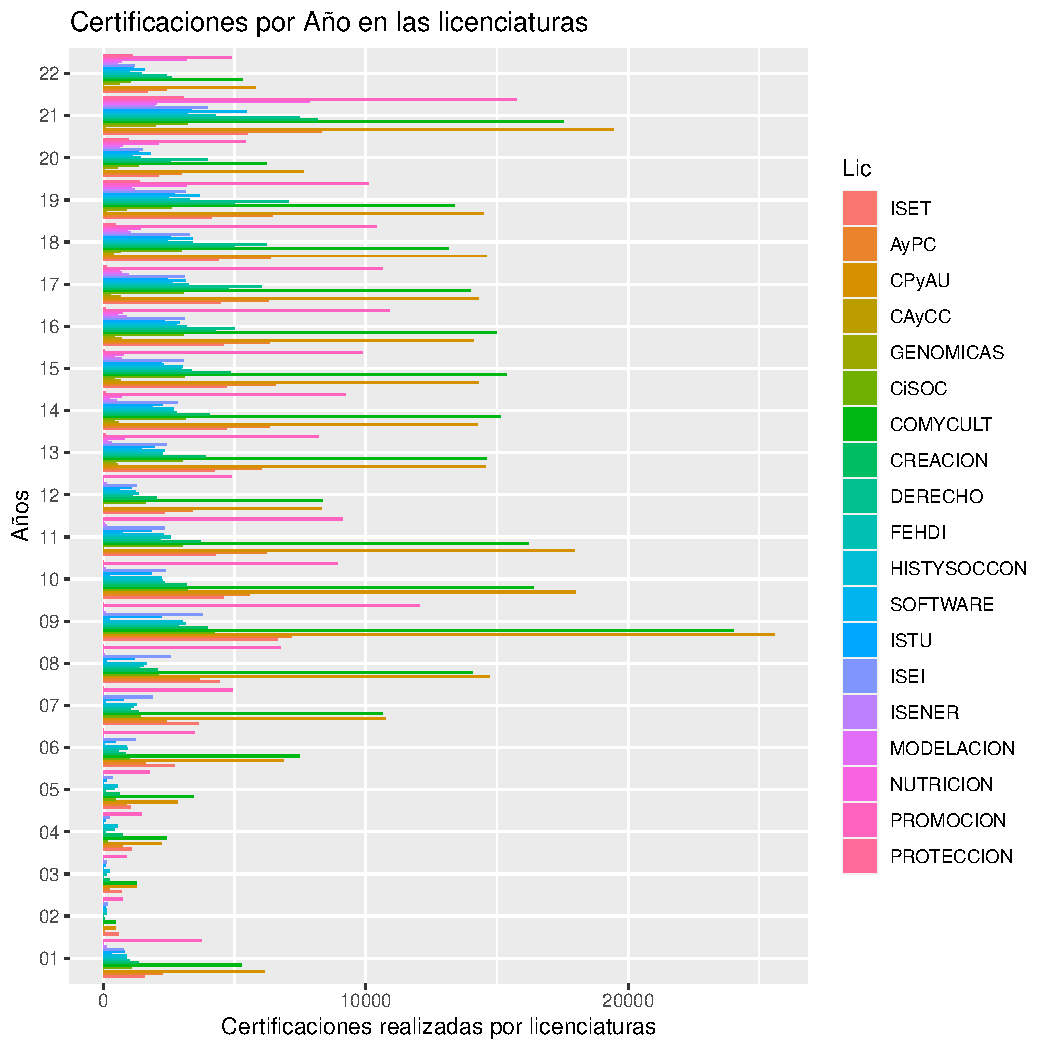
\includegraphics[scale=0.45]{Graficas/ggplotBarplotAnhoLic2.pdf}
\caption{Certificaciones por A\~no por licenciatura}
\label{Fig.Cert.Anho-Lic2}
\end{figure}


El \'area responsable de coordinar y realizar los procesos de evaluaci\'on de conocimientos con fines de certificaci\'on, ya sea para materias espec\'ificos, ciclos e incluso de titulaci\'on es la Coordinaci\'on de Certificaci\'on y registro, \cite{ProyectoEducativo}.


\begin{figure}
\centering
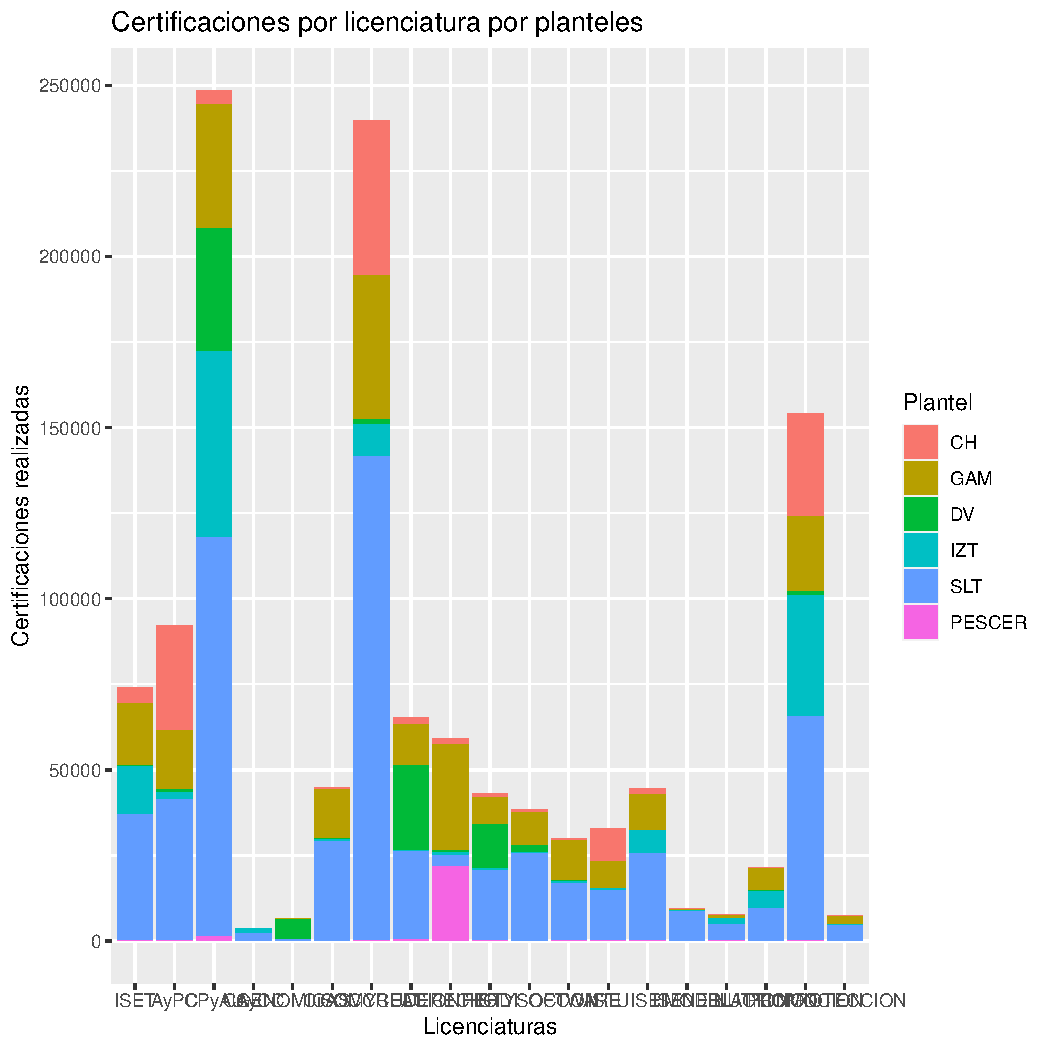
\includegraphics[scale=0.45]{Graficas/ggplotBarplotLicPlantel.pdf}
\caption{Certificaciones por licenciatura por plantel}
\label{Fig.Cert.Lic-Plantel}
\end{figure}

Formalmente la certificaci\'on se define como el proceso mediante el cual la Universidad Aut\'onoma de la Ciudad de M\'exico eval\'ua los conocimientos y competencia con que cuenta el y la estudiante \cite{CircularCertificacion}.

\begin{figure}
\centering
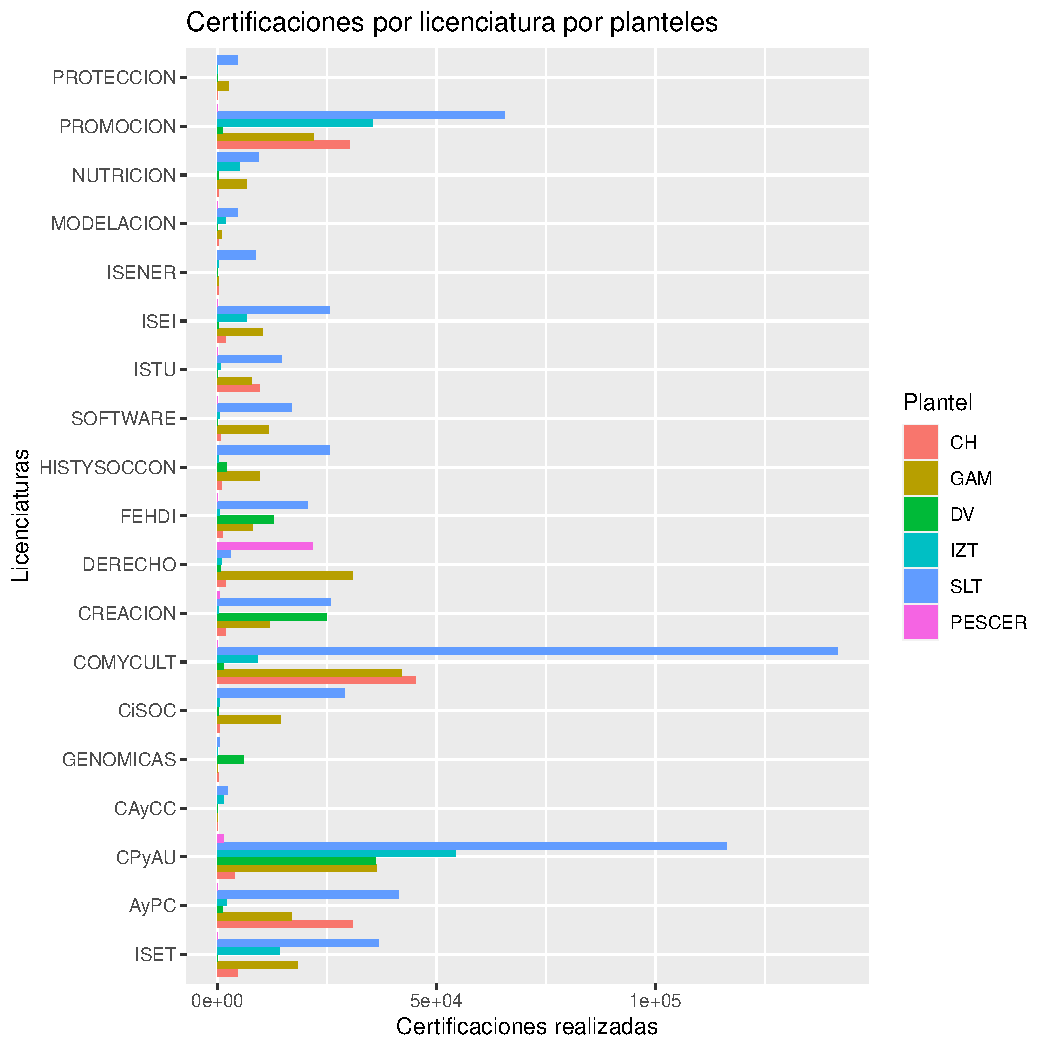
\includegraphics[scale=0.45]{Graficas/ggplotBarplotLicPlantel2.pdf}
\caption{Certificaciones por licenciatura por plantel}
\label{Fig.Cert.Lic-Plantel2}
\end{figure}


La certificaci\'on es aplicada por comit\'es de certificaci\'on, grupo colegiado integrado por profesores investigadores y profesoras investigadoras  nombradas por las academias,  conforme lo establece la circular para regular los procesos y procedimientos de certificaci\'on \cite{CircularCertificacion}.

\begin{figure}
\centering
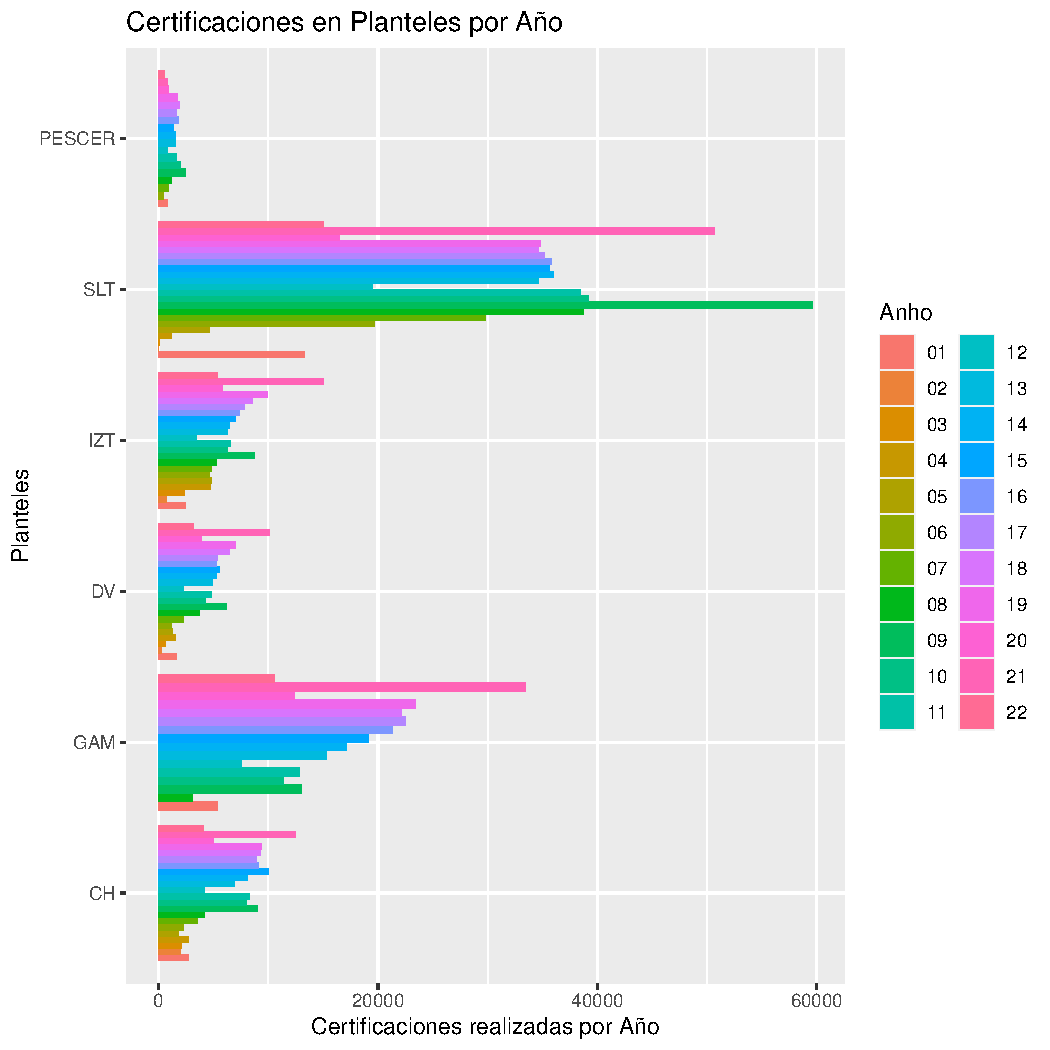
\includegraphics[scale=0.45]{Graficas/ggplotBarplotPlantelAnho.pdf}
\caption{Certificaciones por plantel por anho}
\label{Fig.Cert.Plantel-Anho}
\end{figure}


Actualmente se cuenta con distintas modalidades de certificaci\'on que pueden ser desde: elaboraci\'on de un portafolio,  proyectos, carpetas de trabajo,  presentaci\'on de un \'unico examen de evaluaci\'on de contenidos conforme al programa de estudios.

\begin{figure}
\centering
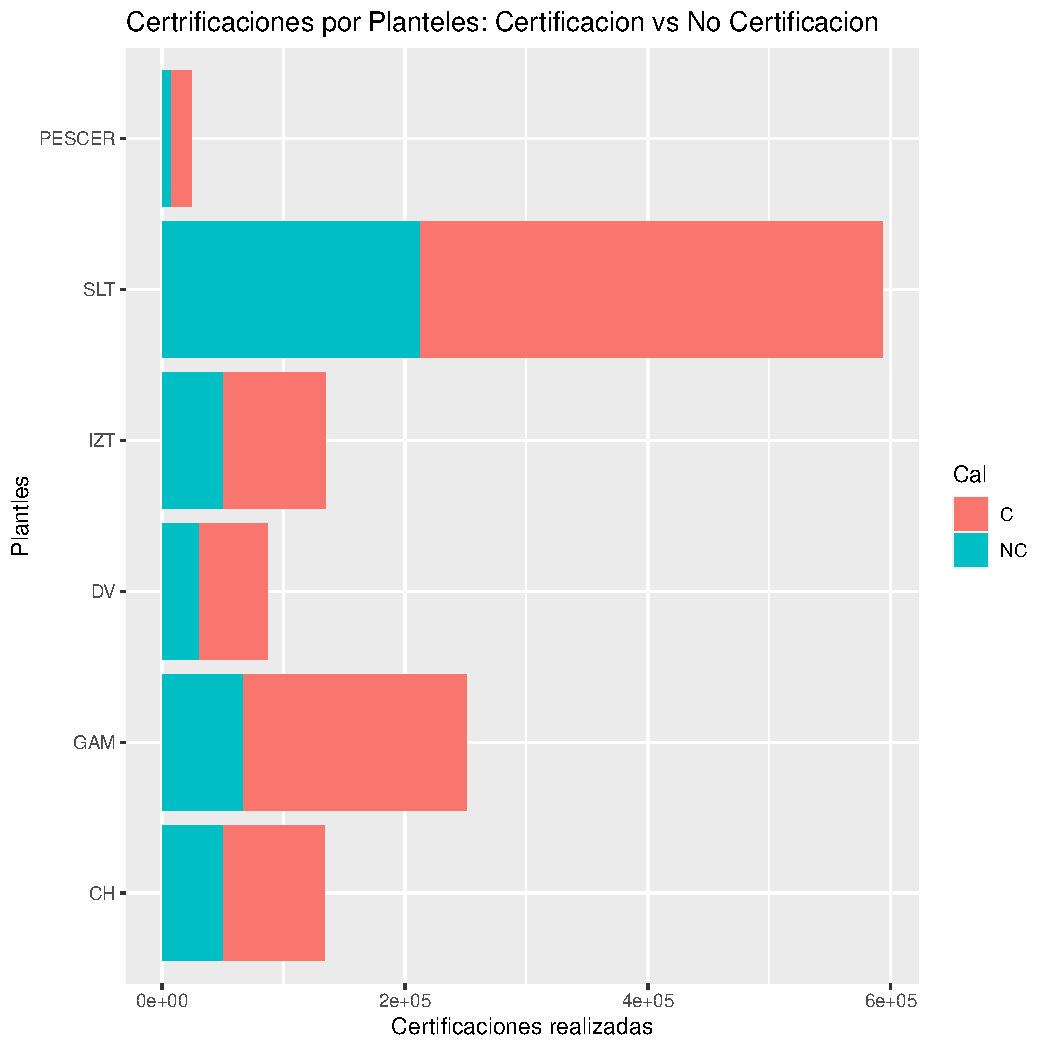
\includegraphics[scale=0.45]{Graficas/ggplotBarplotPlantelCal.pdf}
\caption{Certificaciones por plantel por calificacion}
\label{Fig.Cert.Plantel-Cal}
\end{figure}

\textbf{Aspectos importantes de la certificaci\'on son: las y los estudiantes pueden presentarse cuantas veces lo consideren necesario, las pruebas se basan en el programa del curso, \cite{Doc3}}.


\begin{figure}
\centering
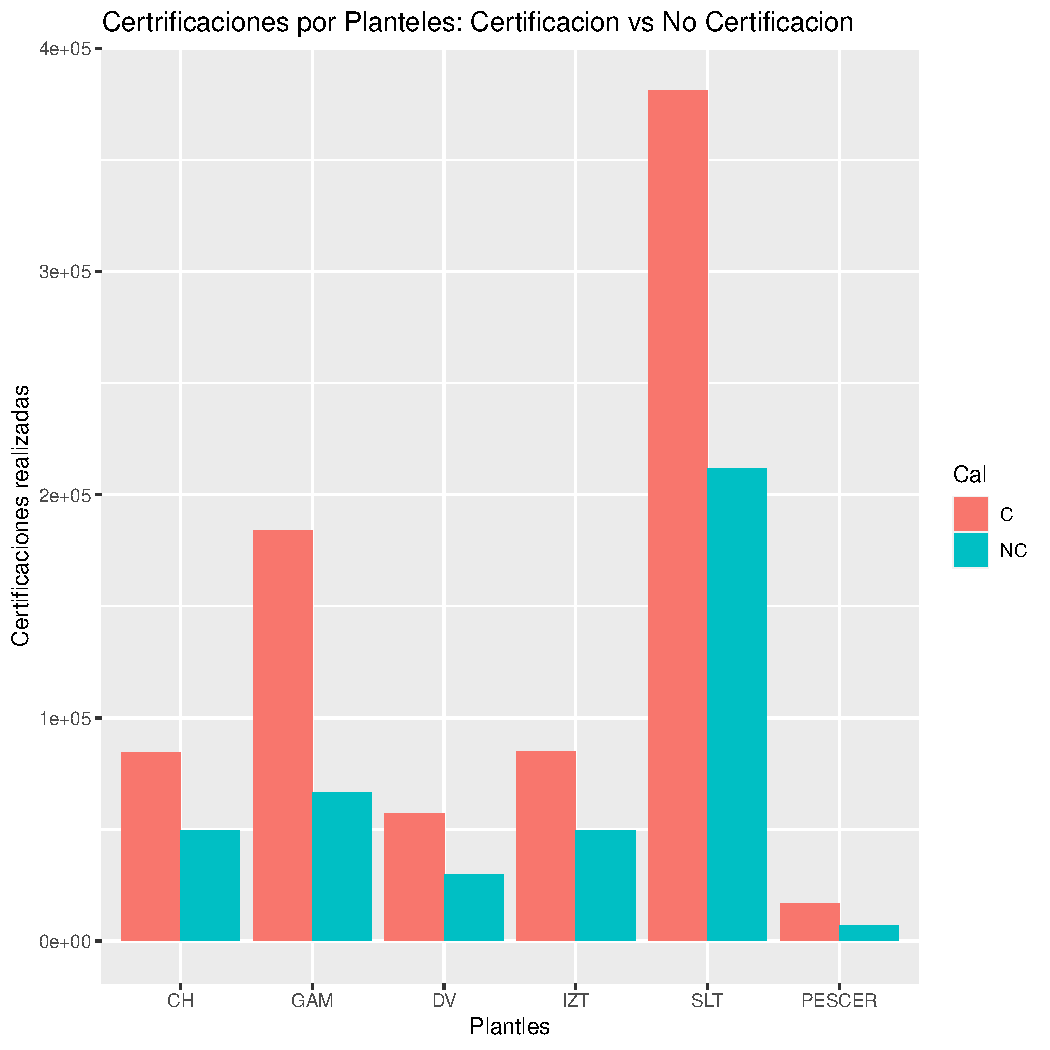
\includegraphics[scale=0.45]{Graficas/ggplotBarplotPlantelCal2.pdf}
\caption{Certificaciones por plantel por calificacion}
\label{Fig.Cert.Plantel-Cal2}
\end{figure}



\section{Descripci\'on del Problema}

\begin{figure}
\centering
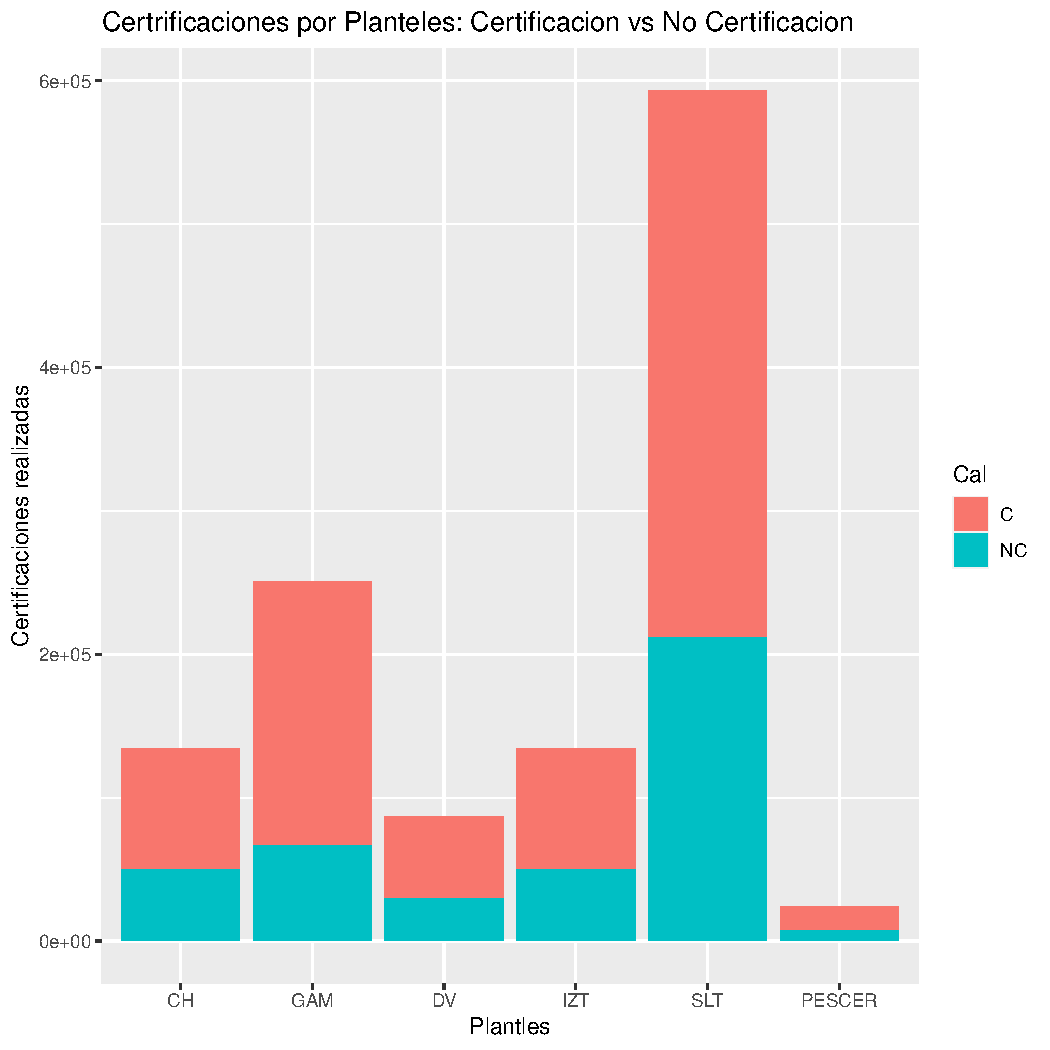
\includegraphics[scale=0.45]{Graficas/ggplotBarplotPlantelCal3.pdf}
\caption{Certificaciones por plantel por calificacion}
\label{Fig.Cert.Plantel-Cal3}
\end{figure}


Actualmente la Universidad ha ofertado hasta 1332 distintas materias desde su creaci\'on, algunas de ellas han cambiado su nombre, algunas otras a traves de la modificaci\'on del programa de estudio se han dividido en dos materias, como es el caso de la materia de C\'alculo Diferencial e Integral, que ahora son dos cursos distintos: C\'alculo Diferencial y C\'alculo Integral.


\begin{figure}
\centering
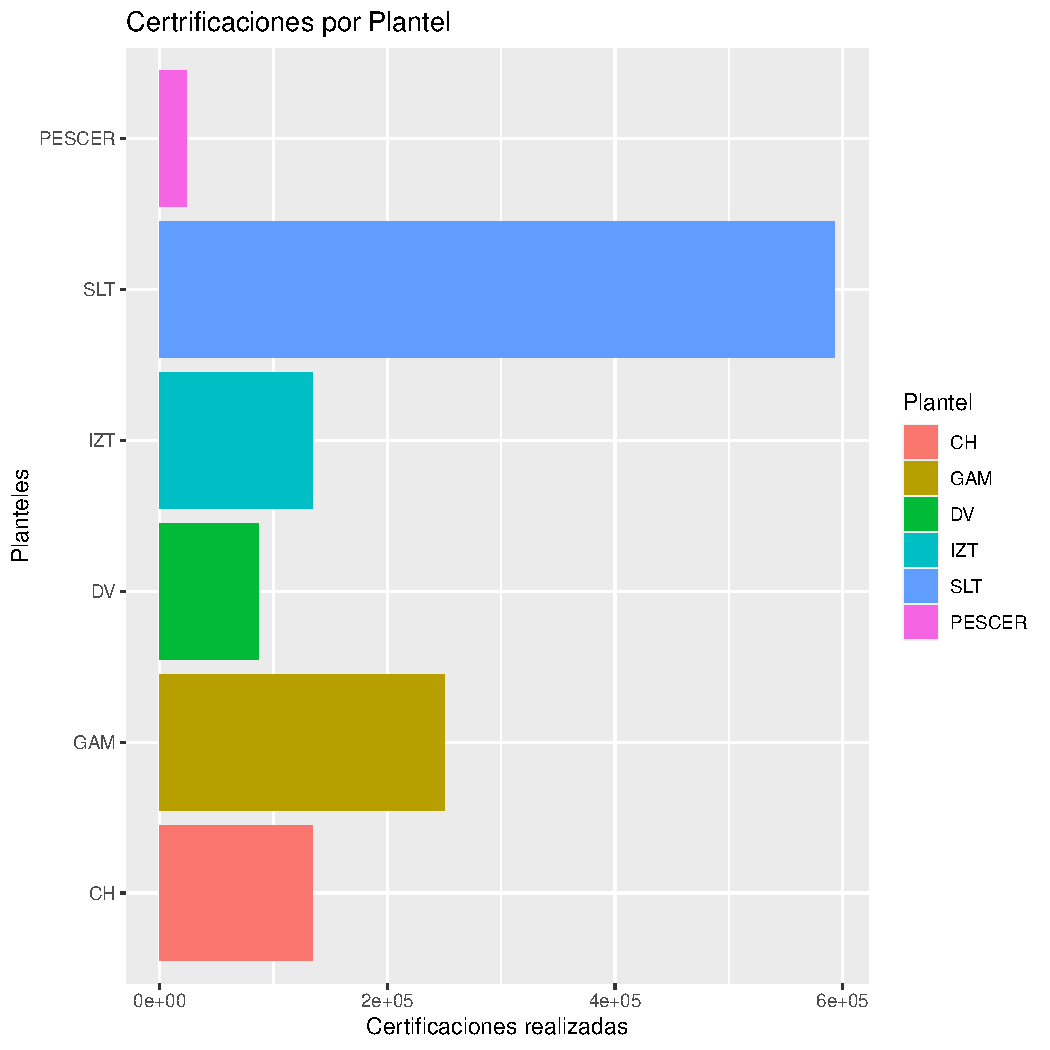
\includegraphics[scale=0.45]{Graficas/ggplotBarplotPlanteles.pdf}
\caption{Certificaciones por planteles}
\label{Fig.Cert.Plantel}
\end{figure}

La informaci\'on se encontraba concentrada en dos archivos con m\'as de un mill\'on de entradas con 10 columnas en un archivo y m\'as de doscientos mil entradas en otro archivo con la misma cantidad de columnas, en las cuales se inclu\'ia la generaci\'on a la que pertenece el estudiantes, su matr\'icula, el nombre de la carrera en curso,  plantel de adscripci\'on, turno, situaci\'on (suspensi\'on tempora, titulado,   activo,  egresado,  baja definitiva o baja temporal), materia, tema espec\'ifico, calificaci\'on y periodo de certificaci\'on.


\begin{figure}
\centering
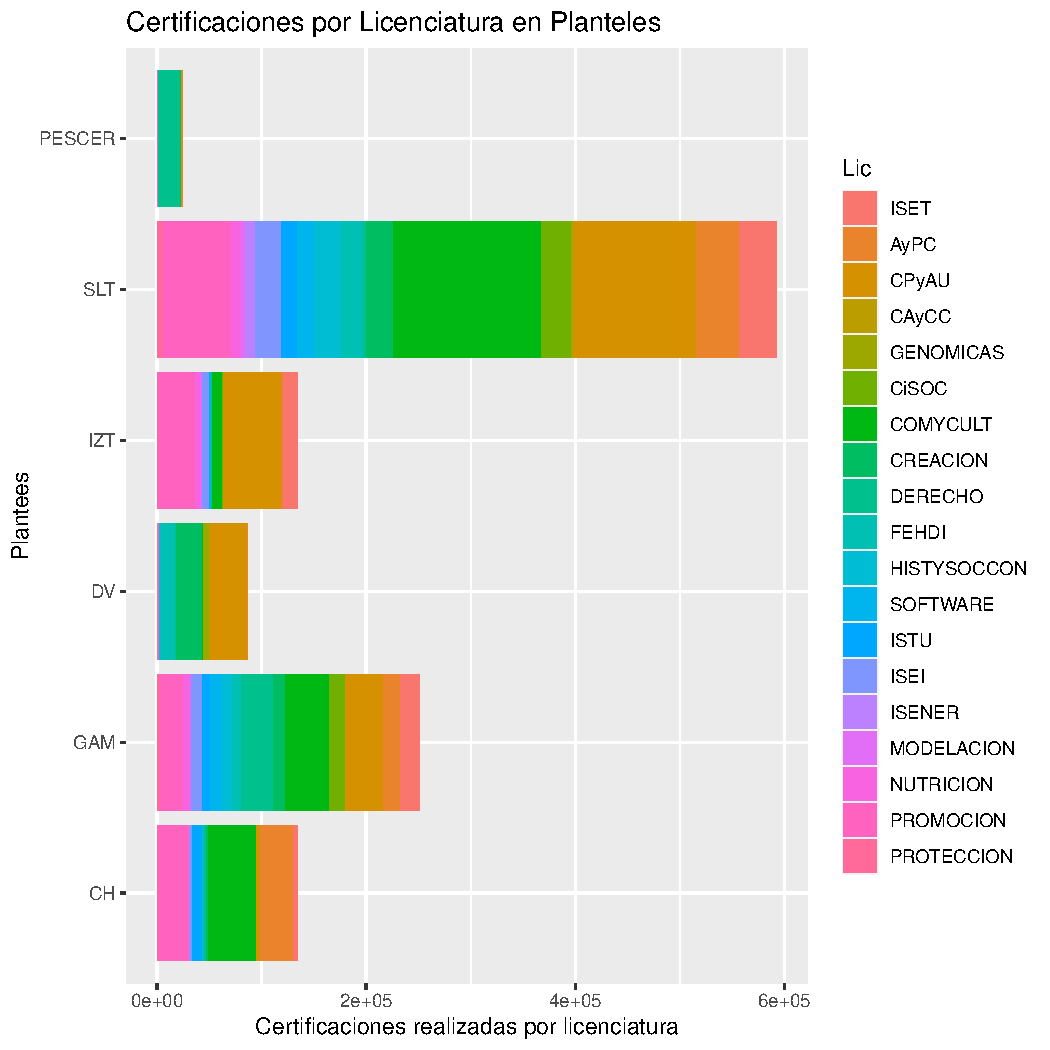
\includegraphics[scale=0.45]{Graficas/ggplotBarplotPlantelLic.pdf}
\caption{Certificaciones por planteles por licenciaturas}
\label{Fig.Cert.Plantel-Lic}
\end{figure}




Los datos considerados son desde la generaci\'on 1 hasta la generaci\'on 21, es decir, todas aquellas personas estudiantes que se han inscrito en la Universidad para cualquiera de las licenciaturas que se ofrecen: Ingenier\'ia en Sistemas Electr\'onicos y de Telecomunicaciones, Arte y Patrimonio Cultural, Ciencia Pol\'itica y Administraci\'on Urbana, Ciencias Ambientales y Cambio Clim\'atico, Ciencias Gen\'omicas, Ciencias Sociales, Comunicaci\'on y Cultura, Creaci\'on Literaria, Derecho, Filosof\'ia e Historia de las Ideas, Historia y Sociedad Contempor\'anea, Ingenier\'ia de Software, Ingenier\'ia en Sistemas de Transporte Urbano, Ingenier\'ia en Sistemas Electr\'onicos Industriales, Ingenier\'ia en Sistemas Energ\'eticos, Modelaci\'on Matem\'atica, Nutrici\'on y Salud, Promoci\'on de la Salud y  Protecci\'on Civil y Gesti\'on de Riesgos.

\begin{figure}
\centering
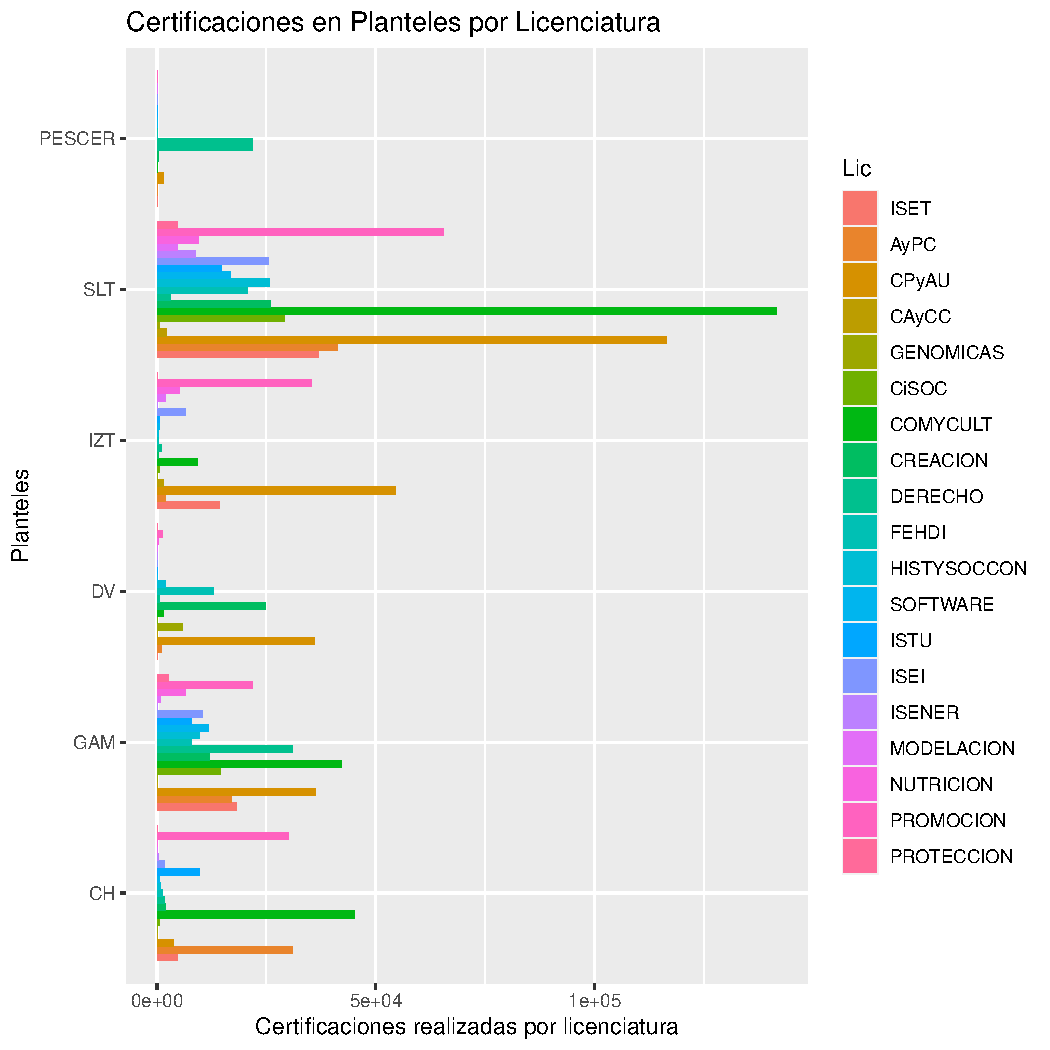
\includegraphics[scale=0.45]{Graficas/ggplotBarplotPlantelLic2.pdf}
\caption{Certificaciones por planteles por licenciatura}
\label{Fig.Cert.Plantel-Lic2}
\end{figure}



Dada la cantidad de informaci\'on y ante la necesidad de unificar ambas bases de datos, se opt\'o por trabajar en \textit{R commander}, lo cual permiti\'o codificar y procesar las variables y datos a estudiar.




Una vez unificadas ambas bases de datos se realizaron las siguientes acciones:
Para la variable Planteles, se consideraron los cinco planteles en los que se imparten cursos: Centro Hist\'orico, Cuautepec, Del Valle, Iztapalapa, San Lorenzo Tezonco; y todos los dem\'as (Reclusorio Preventivo Varonil Norte, Centro Escolar Dr. Pedro L\'opez Penitenciar\'ia del Distrito Federal, Centro Escolar Francisco I Madero Centro Femenil de Readaptaci\'on Social de Tepepan, Centro Escolar Francisco I Madero Ceresova Centro de Readaptaci\'on Social Varonil Oriente, Centro Escolar Jos\'e Vasconcelos Ceresova Centro de Readaptaci\'on Social Varonil Sur, Centro Escolar Rosario Ibarra de Piedra Cefereso Centro Femenil de Readaptaci\'on Social Santa Martha Acatitla, Centro Escolar Santiago Ram\'irez, Centro Escolar Valent\'in Campa Salazar Ceresova Centro de Readaptaci\'on Social Varonil Santa Martha Acatitla) se concentraron en una sola variable: PESCER.

La variable Calificaci\'on se consideraron los valores 7,8,9 y 10 como \textit{Certificada}, y los valores No Present\'o y No Certific\'o como \textit{No Certificada}, la raz\'on es que la/el estudiantes se registr\'o para certificaci\'on y aunque no se haya presentado se considera como un intento de certificaci\'on no exitoso.

                  
El tratamiento para la variable Materia fue un poco m\'as laborioso, con la finalidad de tener \'unicamente texto plano se eliminaron acentos, las min\'usculas se convirtieron en may\'usculas, se eliminaron comilllas, comas y diagonales, se eliminaron las \~ns y di\'eresis. Una vez terminado es preprocesamiento, se ordenaron para contar el n\'umero efectivo de materias registradas en el sistema.

En lo que corresponde a la variable Tema Espec\'ifico, al igual que la anterior se eliminaron acentos, di\'eresis, \~ns, diagnoales, se convirti\'o todo a may\'usculas, y finalmente, aquellos valores ausentes se cubrieron por su respectivo valor en la variable Materia, es decir, la variable \textit{Tema Espec\'ifico} incluye todos los nombres de las materias junto con los nombres de los seminarios o materias optativas ofertadas en alg\'un momento.

Para la variable Periodo de Certificacion su tratamiento fue diferente, primero se proceso cada uno de los datos para que el programa lo pudiera leer efectivamente como fecha, una vez logrado lo anterior, se codific\'o en dos valores: primer y segundo, haciendo referencia al periodo de certificaci\'on correspondiente al primer o segundo semestre del a\~no, uniformizando los distintos valores que estaban registrados de origen. El procesamiento anterior permiti\'o incorporar una nueva variable relacionada con la certificaci\'on: a\~no, misma que se agreg\'o al final de la base de datos.

Es en esta parte del proceso en que se puede considerar que termina el preprocesamiento de datos, para dar pie a la revisión y procesamiento de los datos para obtener de cada materia informaci\'on importante relacionada con la certificaci\

Cada rengl\'on de la base de datos corresponde a una matr\'icula y su respectivo intento (fallido/efectivo) de certificaci\'on para una materia, es decir, puede ocurrir que los primeros 3 renglones correspondan a la misma matr\'icula, misma materia pero distinta calificaci\'on (certificada o no certificada) y distinto periodo de certificaci\'on y distinto a\~no, con lo cu\'al es posible determinar el n\'umero de intentos requeridos para certificar la materia, en caso de que lo haya logrado, cuantos intentos de certificaci\'on realiz\'on sin \'exito, es decir, sin haber logrado certificar la materia; tambien es posible determinar si pudo certificar en su primer intento. Esto se hace para cada estudiante y para cada materia registrada en su historial acad\'emico. 


En esta primera aproximaci\'on se decidi\'o que era de inter\'es conocer para cada materia cuales eran las probabilidades de certificar al primer intento, cu\'al es la probabilidad de no certificar nunca la materia, as\'i como informaci\'on  relacionada con los intentos necesarios para certificar la materia.

Para el caso de no certificar nunca, se calcularon las tres medidas de tendencia central, as\'i como el valor m\'aximo para los intentos fallidos realizados por certificar la materia.



Para el caso de materia s\'i certificada, de manera an\'aloga se calcularon las medidas de tendencia central y el n\'umero m\'aximo de intentos realizados para poder certificar la materia en su \'ultimo intento. 

Adem\'as de lo anterior, para cada materia se extrajeron y almacenaron subbases de datos con toda la informaci\'on sin procesar para la materia en turno, un archivo con una tabla de conteo de la informaci\'on correspondiente a la no certificaci\'on, an\'alaogamente para el caso de s\'i certificaci\'on pero no en el primer intento. 


\section{Ap\'endice: Tablas}


\begin{table}[ht]
\centering
\scalebox{0.75}[.85]{
\begin{tabular}{rrrrrrr}
  \hline
 & CH & GAM & DV & IZT & SLT & PESCER \\ 
  \hline
01 & 8263 & 146 & 2321 & 4707 & 1430 &   0 \\ 
  02 & 4132 & 326 & 2328 & 11398 & 5101 &   0 \\ 
  03 & 1235 & 241 & 1006 & 5370 & 12801 &   0 \\ 
  04 & 2173 & 697 & 3130 & 1191 & 31416 &   0 \\ 
  05 & 9193 & 1476 & 2647 & 8157 & 80933 & 2794 \\ 
  06 & 10566 & 1852 & 11588 & 7523 & 64603 & 1029 \\ 
  07 & 9718 & 21549 & 4843 & 7076 & 38846 & 1844 \\ 
  08 & 8183 & 22348 & 3749 & 6545 & 36801 & 2399 \\ 
  09 & 7756 & 15305 & 3881 & 5612 & 33917 & 2020 \\ 
  10 & 7005 & 12963 & 4311 & 5406 & 31698 & 2342 \\ 
  11 & 6653 & 16435 & 5044 & 5656 & 29265 & 1368 \\ 
  12 & 7688 & 24588 & 5988 & 8342 & 35439 & 1615 \\ 
  13 & 8749 & 19903 & 6007 & 6911 & 32264 & 2750 \\ 
  14 & 9753 & 20987 & 4963 & 7590 & 31143 & 217 \\ 
  15 & 8400 & 23058 & 4558 & 7571 & 29166 & 2071 \\ 
  16 & 6383 & 18276 & 5165 & 8166 & 25932 & 1011 \\ 
  17 & 7120 & 17947 & 6180 & 8601 & 25392 & 825 \\ 
  18 & 4928 & 14830 & 4321 & 8548 & 21391 & 1474 \\ 
  19 & 3727 & 9678 & 2962 & 5775 & 13907 & 206 \\ 
   \hline
\end{tabular}}
\caption{\label{Cert_Gen_Plantel}Certificaci\'on en planteles por generaci\'on.}
\end{table}



\begin{table}[ht]
\centering
\begin{tabular}{||r||r||r|r||}\hline
\multicolumn{4}{|c|}{Certificaciones} \\\hline
Año  & Cantidad  & Año  & Cantidad  \\\hline
01 & 26173& 12 & 3774 \\ 
  02 & 2927 &13 & 69575  \\ 
  03 & 5109 & 14 & 74449\\ 
  04 & 10144 & 15 & 78721\\ 
  05 & 12565 &16 & 80783 \\ 
  06 & 28147 &17 & 81429\\ 
  07 & 41332 &18 & 82974\\ 
  08 & 56299 &19 & 86330\\ 
  09 & 99032 &20 & 44395\\ 
  10 & 71193 &21 & 122594 \\ 
  11 & 72554 &22 & 38627\\
\hline
\end{tabular}
\caption{\label{CertificacionesAnual}n\'umero de certificaciones por a\~no en toda la Universidad.}
\end{table}

\begin{table}[ht!]
\centering
\scalebox{0.75}[.85]{
\begin{tabular}{rr}
  \hline
 & V1 \\ 
  \hline
CH & 134038 \\ 
  GAM & 250641 \\ 
  DV & 86983 \\ 
  IZT & 134405 \\ 
  SLT & 593060 \\ 
  PESCER & 23965 \\ 
   \hline
\end{tabular}
}
\caption{\label{Prob_Cert_Intento_1}Probabilidad de certificar en el primer intento.}
\end{table}


\begin{table}[ht]
\centering
\scalebox{0.75}[.75]{
\begin{tabular}{||c||rrrrrr||rrrrrr||}
\hline\hline
\multicolumn{1}{||c||}{\multirow{3}{*}{AÑO}} & \multicolumn{12}{c||}{Certificaciones}                                                                                                                                                                                                                                                                                               \\ \cline{2-13} 
\multicolumn{1}{||c||}{}& \multicolumn{6}{c||}{Favorables}                                                                                                                                  & \multicolumn{6}{c||}{No Favorables}                                                                                                                               \\ \cline{2-13} 
\multicolumn{1}{||c||}{}& \multicolumn{1}{l|}{CH} & \multicolumn{1}{l|}{GAM} & \multicolumn{1}{l|}{DV} & \multicolumn{1}{l|}{IZT} & \multicolumn{1}{l|}{SLT} & \multicolumn{1}{l||}{PESCER} & \multicolumn{1}{l|}{CH} & \multicolumn{1}{l|}{GAM} & \multicolumn{1}{l|}{DV} & \multicolumn{1}{l|}{IZT} & \multicolumn{1}{l|}{SLT} & \multicolumn{1}{l||}{PESCER} \\ \hline
01 &  1709 & 3950 & 1046 & 1636 & 9562 & 498&  980 & 1388 &  557 &  826 & 3752  &  269\\
  02 & 466 & 0 & 114 & 258 & 2 & 0& 1510 &    0  & 120 &  448 &    9  &    0\\
  03 & 1051 & 0 & 426 & 1347 & 48 & 0 & 1062 &    0  & 159 &  996 &   20  &    0\\
  04 & 1493 & 0 & 1234 & 2164 & 656 & 0& 1222 &    0  & 289 & 2548 &  538  &    0\\
  05 & 896 & 0 & 814 & 2340 & 2299 & 0&  939 &    0  & 465 & 2503 & 2309  &    0\\
  06 & 1075 & 0 & 646 & 2287 & 8854 & 343& 1195 &    0  & 494 & 2325 &10799  &  129\\
  07 & 1482 & 0 & 1336 & 2391 & 13483 & 614& 2076 &    0  & 921 & 2404 &16304  &  321\\
  08 & 1914 & 1622 & 1903 & 2706 & 18035 & 813& 2300 & 1474 & 1866 & 2598 &20715  &  353\\
  09 & 4447 & 6951&3302&  4559 &30956 &  1727& 4528 & 6086 & 2925 & 4222 &28648   &681\\
  10 & 4204 & 7147 & 2585 & 3534& 22883 &  1505& 3851 & 4267 & 1708 & 2716 &16299  &  494\\
  11 & 4850 & 8846 & 2716 & 4179& 25113 &  1112& 3395 & 3976 & 2098 & 2416 &13310  &  543\\
  12 & 2501 & 5264 & 1454 & 2232& 13004  &  510& 1670 & 2279 &  786 & 1185 & 6532  &  323\\
  13 & 4493 &10846 & 3260 & 4031& 24282  & 1071& 2459 & 4449 & 1658 & 2255 &10347  &  424\\
  14 & 5345 &12594 & 3377 & 4153& 24967  & 1153& 2725 & 4519 & 1890 & 2332 &11015  &  379\\
  15 & 6242 &14426 & 3725 & 4557& 25280  & 1055& 3787 & 4667 & 1853 & 2428 &10370  &  331\\
  16 & 6111 &16010 & 3593 & 4872& 25648  & 1417& 2999 & 5349 & 1713 & 2494 &10170  &  407\\
  17 & 6225 &16896 & 3700 & 5320& 24879  & 1346& 2710 & 5607 & 1623 & 2487 &10312  &  324\\
  18 & 6686 &17182 & 4496 & 5854& 24555  & 1432& 2596 & 4997 & 1932 & 2712 &10105  &  427\\
  19 & 6950 &18591 & 5026 & 6946& 25053  & 1384& 2424 & 4863 & 2007 & 2999 & 9745  &  342\\
  20 & 3487 & 9168 & 2559 & 4015& 11794  &  322& 1470 & 3183 & 1333 & 1774 & 4684  &  606\\
  21 & 9585 &26384 & 7514 &11323& 38172  &  248& 2873 & 7111 & 2623 & 3689 &12502  &  570\\
  22 & 3104 & 8335 & 2274 & 4060& 11610  &  304&  951 & 2214 &  863 & 1284 & 3440  &  188\\\hline\hline
\end{tabular}}
\caption{Numero de certificaciones por a\~no en cada uno de los planteles de la universidad}
\label{Tabla_Certificaciones_Plantel_Anho}
\end{table}



\begin{table}[ht!]
\centering
\scalebox{0.75}[.85]{
\begin{tabular}{lrrrrrrrrrr}
  \hline\hline
Licenciatura & 01 & 02 & 03 & 04 & 05 & 06 & 07 & 08 & 09 & 10\\ 
  \hline
ISET & 2049 & 2419 & 1948 & 2392 & 10023 & 7398 & 5667 & 5259 & 4571 & 3414 \\ 
  AyPC & 609 & 1689 & 1551 & 3076 & 7340 & 4206 & 7513 & 8282 & 5824 & 6238\\ 
  CPyAU & 3032 & 6797 & 3248 & 8669 & 26126 & 28141 & 19151 & 17680 & 14577 & 13071\\ 
  CAyCC &   0 &   0 &   0 &   0 &   0 &   0 &   0 &   0 &   0 &   0\\ 
  GENOMICAS &   0 &   0 &   0 &   0 &   0 &   0 &   0 &   0 &   0 &  50\\ 
  CiSOC &  14 & 122 & 1464 & 1542 & 3352 & 2761 & 4017 & 4070 & 3364 & 2655\\ 
  COMYCULT & 3605 & 7303 & 5908 & 7418 & 26558 & 22101 & 19832 & 16680 & 15086 & 12666\\ 
  CREACION & 555 & 518 & 1158 & 2567 & 3062 & 4595 & 3586 & 4146 & 4088 & 4235\\ 
  DERECHO &  69 & 372 & 496 & 438 & 3562 & 1367 & 2642 & 3214 & 2765 & 3434\\ 
  FEHDI & 603 & 228 & 807 & 3095 & 2469 & 2495 & 2433 & 3534 & 2091 & 2065\\ 
  HISTYSOCCON & 772 & 341 & 1241 & 1998 & 2353 & 2675 & 1924 & 2485 & 2194 & 2491\\ 
  SOFTWARE &   0 &  13 &   0 &  58 & 242 & 495 & 166 & 302 & 528 & 1814\\ 
  ISTU & 362 & 378 & 259 & 1257 & 2507 & 2758 & 2039 & 2576 & 1787 & 1841\\ 
  ISEI & 402 & 721 & 801 & 1987 & 5832 & 4130 & 4049 & 1931 & 2191 & 1479\\ 
  ISENER &   0 &   0 &   0 &  70 &   0 & 230 & 171 & 249 & 307 & 274\\ 
  MODELACION &  10 &   0 &   0 &   2 &  45 &  38 &  72 &  28 &  50 &  40\\ 
  NUTRICION &   0 &   2 &   1 &   0 &  97 &  40 &  19 &  19 &   7 & 132 \\ 
  PROMOCION & 4785 & 2382 & 1771 & 4027 & 11599 & 13731 & 10594 & 9570 & 9013 & 7780\\ 
  PROTECCION &   0 &   0 &   0 &  11 &  33 &   0 &   1 &   0 &  48 &  46\\ 
   \hline\hline
   \hline
\end{tabular}
}
\caption{\label{Prob_Cert_Lic_Gen_1}Certificaciones por generaci\'on en cada una de las licenciaturas (primera parte).}
\end{table}


\begin{table}[ht!]
\centering
\scalebox{0.75}[.85]{
\begin{tabular}{rrrrrrr}
  \hline
 & CH & GAM & DV & IZT & SLT & PESCER \\ 
  \hline
01 & 2689 & 5338 & 1603 & 2462 & 13314 & 767 \\ 
  02 & 1976 &   0 & 234 & 706 &  11 &   0 \\ 
  03 & 2113 &   0 & 585 & 2343 &  68 &   0 \\ 
  04 & 2715 &   0 & 1523 & 4712 & 1194 &   0 \\ 
  05 & 1835 &   0 & 1279 & 4843 & 4608 &   0 \\ 
  06 & 2270 &   0 & 1140 & 4612 & 19653 & 472 \\ 
  07 & 3558 &   0 & 2257 & 4795 & 29787 & 935 \\ 
  08 & 4214 & 3096 & 3769 & 5304 & 38750 & 1166 \\ 
  09 & 8975 & 13037 & 6227 & 8781 & 59604 & 2408 \\ 
  10 & 8055 & 11414 & 4293 & 6250 & 39182 & 1999 \\ 
  11 & 8245 & 12822 & 4814 & 6595 & 38423 & 1655 \\ 
  12 & 4171 & 7543 & 2240 & 3417 & 19536 & 833 \\ 
  13 & 6952 & 15295 & 4918 & 6286 & 34629 & 1495 \\ 
  14 & 8070 & 17113 & 5267 & 6485 & 35982 & 1532 \\ 
  15 & 10029 & 19093 & 5578 & 6985 & 35650 & 1386 \\ 
  16 & 9110 & 21359 & 5306 & 7366 & 35818 & 1824 \\ 
  17 & 8935 & 22503 & 5323 & 7807 & 35191 & 1670 \\ 
  18 & 9282 & 22179 & 6428 & 8566 & 34660 & 1859 \\ 
  19 & 9374 & 23454 & 7033 & 9945 & 34798 & 1726 \\ 
  20 & 4957 & 12351 & 3892 & 5789 & 16478 & 928 \\ 
  21 & 12458 & 33495 & 10137 & 15012 & 50674 & 818 \\ 
  22 & 4055 & 10549 & 3137 & 5344 & 15050 & 492 \\ 
   \hline
\end{tabular}}
\caption{\label{Prob_Cert_Plantel_Anho}Certificaciones por a\~no en cada uno de los planteles} 
\end{table}


\begin{table}[ht!]
\centering
\scalebox{0.75}[.85]{
\begin{tabular}{rrr}
  \hline
 & C & NC \\ 
  \hline
CH & 84316 & 49722 \\ 
  GAM & 184212 & 66429 \\ 
  DV & 57100 & 29883 \\ 
  IZT & 84764 & 49641 \\ 
  SLT & 381135 & 211925 \\ 
  PESCER & 16854 & 7111 \\ 
   \hline
\end{tabular}}
\caption{\label{Prob_Cert_Plantel}Certificaciones en cada uno de los planteles}
\end{table}




\begin{table}[ht!]
\centering
\scalebox{0.75}[.85]{
\begin{tabular}{lrrrrrrrrr}
  \hline
  \hline  
Licenciatura & 11 & 12 & 13 & 14 & 15 & 16 & 17 & 18 & 19 \\ 
  \hline\hline
ISET & 3390 & 4848 & 3896 & 3430 & 4067 & 2555 & 2168 & 2075 & 1312 \\ 
  AyPC & 5021 & 6123 & 5878 & 6302 & 5291 & 5088 & 4566 & 3382 & 2473 \\ 
  CPyAU & 11905 & 13551 & 13760 & 14186 & 11377 & 12614 & 10365 & 9069 & 6888\\ 
  CAyCC &  136 & 3573 &  91 &   0 &   0 &   0 &   0 &   0 &   0 \\ 
  GENOMICAS &  78 & 2012 &   0 &   5 & 142 & 675 & 2144 & 880 & 368\\ 
  CiSOC &  2705 & 3276 & 2917 & 2019 & 2953 & 2262 & 2145 & 1213 & 1111\\ 
  COMYCULT & 12157 & 14780 & 13583 & 14041 & 12104 & 9075 & 10096 & 8153 & 5379\\ 
  CREACION & 5013 & 3615 & 4092 & 4700 & 4264 & 4031 & 3585 & 3262 & 2019\\ 
  DERECHO &  2498 & 3192 & 5669 & 4360 & 8397 & 6215 & 4303 & 3992 & 1285\\ 
  FEHDI & 2704 & 2399 & 3542 & 2753 & 3206 & 2212 & 2527 & 1656 & 1195\\ 
  HISTYSOCCON & 2786 & 3071 & 2512 & 3007 & 2218 & 1535 & 1805 & 1462 & 860\\ 
  SOFTWARE & 2585 & 4804 & 2558 & 3224 & 3539 & 2792 & 2372 & 1724 & 1500\\ 
  ISTU & 2160 & 1884 & 2604 & 2201 & 1988 & 1546 & 1835 & 1255 & 889\\ 
  ISEI & 1700 & 3810 & 2744 & 2635 & 2564 & 2020 & 2091 & 1556 & 878\\ 
  ISENER &827 & 548 & 1140 & 1277 & 1216 & 769 & 673 & 860 & 363\\ 
  MODELACION & 152 & 633 & 673 & 759 & 711 & 963 & 885 & 1069 & 788\\ 
  NUTRICION & 230 & 3410 & 196 & 133 & 538 & 1036 & 4868 & 5255 & 2778\\ 
  PROMOCION & 8368 & 7623 & 10661 & 9614 & 10148 & 9194 & 7785 & 6055 & 5082\\ 
  PROTECCION &  6 & 508 &  68 &   7 & 101 & 351 & 1852 & 2574 & 1087\\ 
   \hline
\end{tabular}
}
\caption{\label{Prob_Cert_Lic_Gen2}Certificaciones por generaci\'on en cada una de las licenciaturas (segund parte).}
\end{table}



\begin{table}[ht]
\centering
\scalebox{0.75}[.85]{
\begin{tabular}{lrrrrrr}
  \hline
 & CH & GAM & DV & IZT & SLT & PESCER \\ 
  \hline\hline
ISET & 4628 & 18211 &  93 & 14183 & 36856 &  29 \\ 
  AyPC & 30861 & 17043 & 1065 & 1988 & 41305 &  38 \\ 
  CPyAU & 3875 & 36315 & 36016 & 54457 & 116407 & 1436 \\ 
  CAyCC &   6 &  15 &  76 & 1465 & 2238 &   0 \\ 
  GENOMICAS & 166 & 119 & 5886 &  62 & 460 &   0 \\ 
  CiSOC & 588 & 14410 & 206 & 588 & 29077 &   0 \\ 
  COMYCULT & 45230 & 42077 & 1413 & 9207 & 141630 & 113 \\ 
  CREACION & 1966 & 11903 & 24891 & 288 & 25837 & 383 \\ 
  DERECHO & 1805 & 30905 & 611 & 1011 & 3095 & 21794 \\ 
  FEHDI & 1151 & 7957 & 12888 & 421 & 20571 &  61 \\ 
  HISTYSOCCON & 884 & 9658 & 2018 & 339 & 25619 &   0 \\ 
  SOFTWARE & 618 & 11688 &  84 & 550 & 16902 &  33 \\ 
  ISTU & 9672 & 7889 &  42 & 626 & 14664 &   5 \\ 
  ISEI & 1772 & 10348 & 166 & 6625 & 25524 &  21 \\ 
  ISENER & 236 & 160 &  59 & 205 & 8701 &   0 \\ 
  MODELACION & 142 & 827 &  61 & 1888 & 4698 &  28 \\ 
  NUTRICION & 211 & 6585 & 234 & 5028 & 9378 &   0 \\ 
  PROMOCION & 30101 & 21931 & 1158 & 35379 & 65514 &  24 \\ 
  PROTECCION & 126 & 2600 &  16 &  95 & 4584 &   0 \\ 
   \hline
\end{tabular}
}
\caption{\label{Cert_Lic_Plantel}Certificaciones por licenciatura en cada uno de los planteles.}
\end{table}



\begin{table}[ht]
\centering
\scalebox{0.75}[.85]{
\begin{tabular}{lrr}
  \hline
 Licenciatura & Certificado & No Certificado \\ 
  \hline
ISET & 40221 & 33779 \\ 
  AyPC & 63532 & 28768 \\ 
  CPyAU & 161383 & 87123 \\ 
  CAyCC & 2865 & 935 \\ 
  GENOMICAS & 4429 & 2264 \\ 
  CiSOC & 30339 & 14530 \\ 
  COMYCULT & 165426 & 74244 \\ 
  CREACION & 46718 & 18550 \\ 
  DERECHO & 43184 & 16037 \\ 
  FEHDI & 27880 & 15169 \\ 
  HISTYSOCCON & 25704 & 12814 \\ 
  SOFTWARE & 19503 & 10372 \\ 
  ISTU & 19246 & 13652 \\ 
  ISEI & 25305 & 19151 \\ 
  ISENER & 6545 & 2816 \\ 
  MODELACION & 4922 & 2722 \\ 
  NUTRICION & 16725 & 4711 \\ 
  PROMOCION & 99276 & 54831 \\ 
  PROTECCION & 5178 & 2243 \\ 
   \hline
\end{tabular}
}
\caption{\label{Cert_Lic_Cal}Certificaciones por licenciatura.}
\end{table}




\begin{table}[ht]
\centering
\scalebox{0.75}[.85]{
\begin{tabular}{lr}
  \hline
 Licenciatura& Certificaciones \\ 
  \hline
ISET & 74000 \\ 
  AyPC & 92300 \\ 
  CPyAU & 248506 \\ 
  CAyCC & 3800 \\ 
  GENOMICAS & 6693 \\ 
  CiSOC & 44869 \\ 
  COMYCULT & 239670 \\ 
  CREACION & 65268 \\ 
  DERECHO & 59221 \\ 
  FEHDI & 43049 \\ 
  HISTYSOCCON & 38518 \\ 
  SOFTWARE & 29875 \\ 
  ISTU & 32898 \\ 
  ISEI & 44456 \\ 
  ISENER & 9361 \\ 
  MODELACION & 7644 \\ 
  NUTRICION & 21436 \\ 
  PROMOCION & 154107 \\ 
  PROTECCION & 7421 \\ 
   \hline
\end{tabular}
}
\caption{\label{Cert_Lic} Certificaciones por licenciatura.}
\end{table}






\begin{table}[ht]
\centering
\scalebox{0.75}[.85]{
\begin{tabular}{rlr}
  \hline
 & Materia & $P[Certificar]$ \\ 
  \hline
1 & APLICACIONES DE ENERGIA NUCLEAR & 1.00 \\ 
  2 & ARGUMENTACION JURIDICA LOS PRINCIPIOS JURIDICOS & 1.00 \\ 
   & EN EL RAZONAMIENTO LEGAL &  \\ 
  3 & BIOPOLITICA Y AUTOINMUNIDAD & 1.00 \\ 
  4 & CAD EN MATEMATICAS & 1.00 \\ 
  5 & CENTRALES GEOTERMICAS & 1.00 \\ 
  6 & CENTRALES HIDROELECTRICAS & 1.00 \\ 
  7 & COMUNIDADES RESILIENTES Y MEDIO AMBIENTE & 1.00 \\ 
  8 & CRISIS MIGRACION Y FRONTERAS (MEXICO-ESTADOS UNIDOS) & 1.00 \\ 
  9 & CULTURAS POPULARES & 1.00 \\ 
  10 & DESARROLLO URBANO INTENSIVO: DISPUTAS POR LA CIUDAD & 1.00 \\ 
  11 & DESPOSESION Y EXPLOTACION EN EL MUNDO CONTEMPORANEO & 1.00 \\ 
  12 & DIDACTICA DE LA EDUCACION AMBIENTAL & 1.00 \\ 
  13 & DISCUSION FILOSOFICA & 1.00 \\ 
  14 & EL CONOCIMIENTO CIENTIFICO DE DA COSTA & 1.00 \\ 
  15 & EL CONOCIMIENTO COMO CONSTRUCCION EN CARNAP & 1.00 \\ 
  16 & EL GNOSTICISMO & 1.00 \\ 
  17 & ELEMENTOS TEORICOS Y METODOLOGICOS DE LA HISTORIA DE LAS IDEAS & 1.00 \\ 
  18 & ETNOALIMENTACION & 1.00 \\ 
  19 & EVALUACION DE POLITICAS PUBLICAS & 1.00 \\ 
  20 & FILOSOFIA Y LITERATURA. ENSAYAR LA REALIDAD & 1.00 \\ 
  21 & FUNDAMENTOS DE ANTROPOLOGIA MOLECULAR Y GENETICA FORENSE & 1.00 \\ 
  22 & GENERO Y POLITICA EN AMERICA LATINA & 1.00 \\ 
  23 & GESTION TRATAMIENTO Y RECUPERACION DE RESIDUOS SOLIDOS & 1.00 \\ 
  24 & INTRODUCCION A LA CREACION LITERARIA III & 1.00 \\ 
  25 & INTRODUCCION A LA INGENIERIA EN SISTEMAS DE TRANSPORTE URBANO & 1.00 \\ 
  26 & INTRODUCCION A LA POESIA OCCIDENTAL SIGLOS XIX Y XX & 1.00 \\ 
  27 & LA CIUDAD DE MEXICO ANTE EL CAMBIO CLIMATICO & 1.00 \\ 
  28 & LA ESCLAVITUD & 1.00 \\ 
  29 & LA TEORIA DEL DON & 1.00 \\ 
  30 & LITERATURA CONTEMPORANEA DEL ESTE DE EUROPA & 1.00 \\ 
  31 & LOGICA DEONTICA & 1.00 \\ 
  32 & LOGICA E INCERTIDUMBRE & 1.00 \\ 
  33 & LOS PUEBLOS ORIGINARIOS DE LA CIUDAD DE MEXICO & 1.00 \\ 
  34 & MICHAEL SANDEL & 1.00 \\ 
  35 & MODELACION DE SISTEMAS FISICOAMBIENTALES II & 1.00 \\ 
  36 & NUEVA RURALIDAD Y POLITICA AGROPECUARIA EN MEXICO & 1.00 \\ 
  37 & PARADIGMA AMBIENTAL Y DESARROLLO SUSTENTABLE & 1.00 \\ 
  38 & PERSPECTIVA DE GENERO Y SUSTENTABILIDAD SOCIAL & 1.00 \\ 
  39 & POESIA II (CURSO TEORICO PRACTICO DE POESIA II) & 1.00 \\ 
  40 & PROBLEMAS DE LOGICA & 1.00 \\ 
  41 & PROBLEMAS INVERSOS II & 1.00 \\ 
  42 & RECUPERACION Y PROMOCION DE AREAS VERDES & 1.00 \\ 
  43 & RELIGION Y MUNDO MODERNO EN LA TEORIA SOCIOLOGICA DE MAX WEBER & 1.00 \\ 
  44 & RUDOLF CARNAP & 1.00 \\ 
  45 & SATELITES DE ORBITAS BAJAS E INTERMEDIAS & 1.00 \\ 
  46 & SEMINARIO DE ANALISIS POLITICO: DISEnO DE TESIS & 1.00 \\ 
  47 & SEMINARIO DE TEXTOS FILOSOFICOS I & 1.00 \\ 
  48 & SEMINARIO MONOGRAFICO III & 1.00 \\ 
  49 & SOCIEDAD CIVIL Y CAMBIO CLIMATICO & 1.00 \\ 
  50 & TALLER DE DIBUJO Y PINTURA & 1.00 \\ 
   \hline
\end{tabular}
}
\caption{\label{Prob_Cert_Intento_1}Probabilidad de certificar en el primer intento.}
\end{table}


\begin{table}[ht]
\centering
\scalebox{0.75}[.85]{
\begin{tabular}{rlr}
  \hline
 & Materia & $P[Certificar]$  \\ 
  \hline 
  51 & VIOLENCIA POLITICA DERECHOS HUMANOS Y MEMORIA EN AMERICA LATINA & 1.00 \\ 
  52 & COMUNICACION PARA LA NUTRICION & 0.99 \\ 
  53 & SEGURIDAD E HIGIENE INDUSTRIAL & 0.99 \\ 
  54 & CIENCIAS DE LA TIERRA Y EVOLUCION DEL CLIMA & 0.98 \\ 
    55 & EDUCACION PARA LA NUTRICION & 0.98 \\ 
  56 & DISEnO BIOCLIMATICO INTEGRAL & 0.98 \\ 
  57 & HISTORIA GENERO Y MUJERES & 0.98 \\ 
  58 & TERMODINAMICA DE LOS ECOSISTEMAS & 0.98 \\ 
  594 & FILOSOFIA Y ETICA AMBIENTAL & 0.98 \\ 
  60 & PROCESOS DEL PETROLEO & 0.98 \\ 
  61 & APROVECHAMIENTO SUSTENTABLE DE RECURSOS NATURALES Y & 0.98 \\ 
  & RECURSOS ECOSISTEMICOS & \\ 
  62 & FARMACOGENOMICA & 0.98 \\ 
  63 & SIN ESPECIFICACION & 0.98 \\ 
  64 & TOPICOS SELECTOS EN INVESTIGACION EN NUTRICION & 0.98 \\ 
  65 & SISTEMA POLITICO Y ELECCIONES EN MEXICO & 0.98 \\ 
  66 & COMBUSTIBLES Y COMBUSTION & 0.98 \\ 
  67 & POLITICA Y RELIGION EN LA CIUDAD DE MEXICO 1977-1994 & 0.97 \\ 
  68 & CIUDADANIA ETNICA E INTERLEGALIDAD & 0.97 \\ 
  69 & ENERGIA Y AMBIENTE & 0.97 \\ 
  70 & GEOPOLITICA DE LA ENERGIA & 0.97 \\ 
  71 & SISTEMAS DE TRATAMIENTO DE AGUA RESIDUALES & 0.97 \\ 
  72 & INSTALACIONES ELECTRICAS & 0.97 \\ 
  73 & PLANES Y PROGRAMAS ALIMENTARIOS NUTRICIONALES & 0.97 \\ 
  74 & PROYECTO DE MODELACION II & 0.97 \\ 
  75 & HISTORIA DE LA LOCURA EN LA EPOCA CLASICA & 0.96 \\ 
  76 & PRINCIPIOS DE INGENIERIA AMBIENTAL & 0.96 \\ 
  77 & RELACIONES INTERNACIONALES CUBA-MEXICO-ESTADOS UNIDOS  & 0.96 \\ 
     & SIGLOS XIX Y XX & \\ 
78 & CRISIS AMBIENTAL CAMBIO CLIMATICO Y SUSTENTABILIDAD & 0.96 \\ 
  79 & PROBLEMA DE LOS RECURSOS HIDRICOS DE MEXICO  & 0.96 \\ 
 & ANTE EL CAMBIO CLIMATICO GLOBAL & \\ 
 80 & EJERCICIO PROFESIONAL DEL NUTRIOLOGO & 0.96 \\ 
  81 & GOBERNABILIDAD Y GOBERNANZA LA DEMOCRACIA EN EL SIGLO XXI & 0.96 \\ 
  82 & SISTEMAS EN TIEMPO REAL & 0.96 \\ 
  83 & ARTHUR SCHOPENHAUER & 0.96 \\ 
  84 & DIETOTERAPIA I & 0.95 \\ 
  85 & GESTION TECNOLOGICA & 0.95 \\ 
  86 & TRABAJO DE INVESTIGACION I & 0.95 \\ 
  87 & PEQUEnAS CENTRALES HIDROELECTRICAS & 0.95 \\ 
  88 & MODELACION MATEMATICA Y COMPUTACIONAL II & 0.95 \\ 
  89 & TRABAJO DE INVESTIGACION II & 0.95 \\ 
  90 & PLANEACION Y DISEnO DE PROGRAMAS DE PROTECCION CIVIL& 0.95 \\ 
 & Y REDUCCION DE RIESGOS & \\ 
  91 & BIOENERGIA & 0.95 \\ 
  92 & ADMINISTRACION DE PROYECTOS I & 0.95 \\ 
  93 & GEOGRAFIA GENERAL & 0.95 \\ 
  94 & ADMINISTRACION DE PROYECTOS II & 0.95 \\ 
  95 & CALIDAD DE LOS SISTEMAS ENERGETICOS & 0.95 \\ 
  96 & ANALISIS DEL TRANSPORTE COMO UN SISTEMA COMPLEJO Y DINAMICO & 0.94 \\ 
  97 & SISTEMAS DE SALUD Y GESTION DE RIESGOS & 0.94 \\ 
  98 & NUTRIGENOMICA & 0.94 \\ 
     \hline
\end{tabular}
}
\caption{\label{Prob_Cert_Intento_2}Probabilidad de certificar en el primer intento (parte 2).}
\end{table}


\begin{table}[ht]
\centering
\scalebox{0.75}[.85]{
\begin{tabular}{rlr}
  \hline
 & Materia & $P[Certificar]$  \\ 
  \hline
  99 & DERECHO Y JUSTICIA AMBIENTAL & 0.94 \\ 
  100 & CRECIMIENTO Y DESARROLLO II (ADULTO TERCERA EDAD) & 0.94 \\ 
  101 & TALLER DE ARTES ESCENICAS I & 0.94 \\ 
  102 & DISEnO Y SISTEMAS DE GESTION AMBIENTAL & 0.94 \\ 
  103 & EPISTEMOLOGIA DE LAS CIENCIAS Y LOS SISTEMAS COMPLEJOS & 0.94 \\ 
  104 & LOGICA VIVA & 0.94 \\ 
  105 & POBLACION Y MEDIO AMBIENTE & 0.94 \\ 
  106 & PROYECTO DE MODELACION I & 0.94 \\ 
  107 & EPIDEMIOLOGIA GENERAL Y NUTRICIONAL & 0.94 \\ 
  108 & BIOENERGIA DE LOS DESECHOS SOLIDOS & 0.94 \\ 
  109 & CELDAS DE MANUFACTURA & 0.94 \\ 
  110 & EDUCACION AMBIENTAL & 0.94 \\ 
  111 & ENERGIAS Y ECOTECNIAS PARA LA MITIGACION& 0.94 \\ 
   & DEL CAMBIO CLIMATICO & \\ 
  112 & METODOS DE EVALUACION DE IMPACTO AMBIENTAL & 0.94 \\ 
  & PARA EL CAMBIO CLIMATICO &  \\ 
  113 & NORMATIVIDAD Y LEGISLACION & 0.94 \\ 
  114 & DERECHO MERCANTIL & 0.94 \\ 
  115 & ONCOGENOMICA & 0.94 \\ 
  116 & COGENERACION & 0.93 \\ 
  117 & FLUJO DE FLUIDOS EN MEDIOS POROSOS & 0.93 \\ 
  118 & PODER GOBIERNO Y ESTADO EN LA HISTORIA  & 0.93 \\ 
   &  DEL PENSAMIENTO POLITICO &  \\ 
  119 & CONVERSION DE LA ENERGIA & 0.93 \\ 
  120 & SEMINARIO DE INTELIGENCIA ARTIFICIAL I: REDES NEURONALES & 0.93 \\ 
  121 & POPULISMOS LATINOAMERICANOS: DECADAS 30 Y 40 & 0.93 \\ 
  122 & TALLER DE ARTES ESCENICAS III & 0.93 \\ 
  123 & HIDROGENO Y CELDAS DE COMBUSTIBLES & 0.93 \\ 
  124 & DESIGUALDAD POBREZA Y DESARROLLO EN AMERICA LATINA & 0.93 \\ 
  125 & LA PHRONESIS DE PLATON & 0.93 \\ 
  126 & TEMAS SELECTOS II & 0.93 \\ 
  127 & NUTRICION COMUNITARIA & 0.93 \\ 
  128 & HISTORIA Y LITERATURA & 0.93 \\ 
  129 & TRANSFERENCIA DE CALOR & 0.92 \\ 
  130 & ESTUDIOS DE ANTROPOLOGIA ECOLOGICA & 0.92 \\ 
  131 & ANALISIS Y MODELAMIENTO DE SOFTWARE & 0.92 \\ 
  132 & INTRODUCCION A LA CREACION LITERARIA I & 0.92 \\ 
  133 & INTRODUCCION A LA CREACION LITERARIA II & 0.92 \\ 
  134 & TALLER DE ARTES POPULARES III & 0.92 \\ 
  135 & SEMINARIO DE TITULACION I & 0.92 \\ 
  136 & GESTION AMBIENTAL Y AUDITORIAS PARA EMPRESAS SUSTENTABLES & 0.92 \\ 
  137 & PLANEACION DEL USO DEL SUELO Y ORDENAMIENTO TERRITORIAL & 0.92 \\ 
  138 & SISTEMAS DE INFORMACION GEOGRAFICA PARA  & 0.92 \\ 
  & EL ANALISIS DEL CLIMA Y MEDIO AMBIENTE & \\ 
 139 & FISIOPATOLOGIA I & 0.92 \\ 
  140 & SEMINARIO DE TITULACION II & 0.92 \\ 
  141 & MATEMATICAS DISCRETAS II & 0.92 \\ 
  142 & GESTION INTEGRAL DE RESIDUOS SOLIDOS & 0.92 \\ 
  143 & GRAHAM PRIEST & 0.92 \\ 
  144 & INTRODUCCION A LA INGENIERIA EN SISTEMAS ENERGETICOS & 0.92 \\ 
  145 & RETORICA DE ARISTOTELES & 0.92 \\ 
     \hline
\end{tabular}
}
\caption{\label{Prob_Cert_Intento_3}Probabilidad de certificar en el primer intento (parte 3).}

\end{table}


\begin{table}[ht]
\centering
\scalebox{0.75}[.85]{
\begin{tabular}{rlr}
  \hline
 & Materia & $P[Certificar]$  \\ 
  \hline
  146 & TEORIA DE LA ARGUMENTACION Y LOGICAS NO CLASICAS & 0.92 \\ 
  147 & VIDEO EXPERIMENTAL & 0.92 \\ 
  148 & BALANCE DE MATERIA Y ENERGIA & 0.92 \\ 
  149 & ESTADISTICA PARA ADMINISTRADORES & 0.92 \\ 
  150 & ESTADISTICA MULTIVARIADA & 0.91 \\ 
  150 & SEMINARIO DE TRABAJO RECEPCIONAL & 0.91 \\ 
  151 & NUTRICION EN EL DEPORTE & 0.91 \\ 
  152 & MAQUINAS ELECTRICAS II & 0.91 \\ 
  153 & INTERCULTURALIDAD DIALOGO DE SABERES Y CONOCIMIENTO INDIGENA & 0.91 \\ 
  154 & TERMODINAMICA AVANZADA & 0.91 \\ 
  155 & SISTEMAS ENERGETICOS ALTERNATIVOS & 0.91 \\ 
  156 & NUTRICION EN EL CICLO DE VIDA & 0.91 \\ 
  157 & PSICOLOGIA SOCIAL II & 0.91 \\ 
  158 & INSTALACIONES TEMPORALES EN CASO DE DESASTRE & 0.91 \\ 
  159 & TRASTORNOS DE LA CONDUCTA ALIMENTARIA & 0.91 \\ 
  160 & CIUDADANIA Y MULTICULTURALISMO & 0.91 \\ 
  161 & EL BANQUETE DE PLATON & 0.91 \\ 
  162 & MECANISMOS DE FINANCIAMIENTO PARA LA RECUPERACION  & 0.91 \\ 
  & EN CASO DE DESASTRES & \\ 
 163 & PROCESOS DESTRUCTIVOS ECOSISTEMICOS Y CRISIS CAPITALISTA MUNDIAL & 0.91 \\ 
  164 & PROCESOS TERMODINAMICOS & 0.91 \\ 
  165 & PATOLOGIA II & 0.91 \\ 
  166 & PEDAGOGIA AMBIENTAL & 0.91 \\ 
  167 & CENTRALES TERMOELECTRICAS & 0.90 \\ 
  168 & FILOSOFIA PRACTICA & 0.90 \\ 
  169 & CLINICA PROCESAL & 0.90 \\ 
  170 & DISEnO DE EXPERIMENTOS EN INGENIERIA DE SOFTWARE & 0.90 \\ 
  171 & MAQUINAS ELECTRICAS I & 0.90 \\ 
  172 & MAQUINAS TERMICAS & 0.90 \\ 
  173 & ESTADISTICA II & 0.90 \\ 
  174 & INTERPRETACION DE TEXTOS & 0.90 \\ 
  175 & JOAQUIN GARCIA ICAZBALCETA Y EMETERIO VALVERDE & 0.90 \\ 
  176 & PROBLEMAS INVERSOS & 0.90 \\ 
  176 & SISTEMAS TERMOSOLARES & 0.90 \\ 
   \hline
\end{tabular}
}\caption{\label{Prob_Cert_Intento_4}Probabilidad de certificar en el primer intento (parte 4).}

\end{table}

\begin{table}[ht]
\centering
\scalebox{0.75}[.85]{
\begin{tabular}{rlr}
  \hline
 & Materia & $P[NoCertificar]$ \\ 
  \hline
1 & ANALISIS SOCIAL Y CULTURAL DE LOS MOVIMIENTOS SOCIALES CULTURALES & 1.00 \\ 
  2 & ESCEPTICISMO ANTIGUA Y MODERNO & 1.00 \\ 
  3 & FILOSOFIA DEL LENGUAJE CLASICO & 1.00 \\ 
  4 & FISICA III & 1.00 \\ 
  5 & INTRODUCCION A LOS ESTUDIOS DEL LENGUAJE: ESCUELAS Y TEORIAS & 1.00 \\ 
  6 & K. O. APEL PRAGMATICA TRASCENDENTAL Y ETICA DISCURSIVA & 1.00 \\ 
  7 & LEGISLACION DEL ARTE Y PATRIMONIO CULTURAL & 1.00 \\ 
  8 & LENGUA EXTRANJERA II & 1.00 \\ 
  9 & LENGUA EXTRANJERA III & 1.00 \\ 
  10 & METODOS CUALITATIVOS & 1.00 \\ 
  11 & PARADIGMA CRITICO & 1.00 \\ 
  12 & QUIMICA ORGANICA (QUIMICA DE LA CELULA) & 1.00 \\ 
  13 & TALLER DE METODOS CUANTITATIVOS & 1.00 \\ 
  14 & LITERATURA CONTEMPORANEA I & 0.93 \\ 
  15 & ADMINISTRACION & 0.92 \\ 
  16 & PROBABILIDAD Y ESTADISTICA & 0.90 \\ 
   \hline
\end{tabular}}
\caption{\label{Prob_No_Cert}Probabilidad de no certificar la materia.}
\end{table}



\begin{table}[ht]
\centering
\scalebox{0.75}[.85]{
\begin{tabular}{rlr}
  \hline
 & Materia & N\'umero Intentos \\ 
  \hline
1 & MECANICA I & 28.00 \\ 
  2 & CALCULO DIFERENCIAL & 19.00 \\ 
3 & CALCULO DIFERENCIAL INTEGRAL & 18.00 \\ 
  4 & ESTUDIOS SOCIALES E HISTORICOS II & 17.00 \\ 
 5 & ESTADISTICA Y PROBABILIDAD & 16.00 \\ 
  6 & ALGEBRA Y GEOMETRIA ANALITICA & 15.00 \\ 
  7 & DISPOSITIVOS ELECTRONICOS I & 15.00 \\ 
  8 & FARMACOLOGIA & 15.00 \\ 
  9 & TEORIA POLITICA II & 15.00 \\ 
  10 & LENGUAJE Y PENSAMIENTO II & 14.00 \\ 
  11 & MECANICA II & 14.00 \\ 
  12 & QUIMICA DE LA CELULA & 14.00 \\ 
  13 & ALGEBRA LINEAL & 13.00 \\ 
  14 & CALCULO INTEGRAL & 13.00 \\ 
  15 & CULTURA CIENTIFICA Y HUMANISTICA II & 13.00 \\ 
  16 & ENFOQUES CRITICOS EN COMUNICACION & 13.00 \\ 
  17 & INGLES II & 13.00 \\ 
  18 & TEORIA POLITICA I & 13.00 \\ 
  19 & CRITICA A LA ILUSTRACION & 12.00 \\ 
  20 & CULTURA CIENTIFICA Y HUMANISTICA I & 12.00 \\ 
  21 & PLANEACION CON PARTICIPACION EN LA CIUDAD DE MEXICO & 12.00 \\ 
  22 & CELULA II & 11.00 \\ 
  23 & CULTURA CIENTIFICA Y HUMANISTICA III & 11.00 \\ 
  24 & DECISION POLITICA Y POLITICAS PUBLICAS & 11.00 \\ 
  25 & INTRODUCCION A LA PROGRAMACION & 11.00 \\ 
  26 & LA INVESTIGACION DE LA PRODUCCION LOS DISCURSOS & 11.00 \\ 
 &  Y LA RECEPCION DE LOS MEDIOS DE COMUNICACION & \\ 
  27 & LENGUAJE Y PENSAMIENTO III & 11.00 \\ 
  28 & TEORIA DE LOS CIRCUITOS & 11.00 \\ 
  29 & ANALISIS POLITICO CON METODOS CUANTITATIVOS & 10.00 \\ 
  30 & BIOESTADISTICA & 10.00 \\ 
  31 & BIOETICA Y VALORES & 10.00 \\ 
  32 & CELULA I & 10.00 \\ 
  33 & CUERPO HUMANO I & 10.00 \\ 
  34 & CUERPO HUMANO II & 10.00 \\ 
  35 & ECUACIONES DIFERENCIALES ORDINARIAS & 10.00 \\ 
  36 & ESTUDIOS SOCIALES E HISTORICOS I & 10.00 \\ 
  37 & HISTORIA DE MEXICO DEL SIGLO XIX & 10.00 \\ 
  38 & INGLES III & 10.00 \\ 
  39 & INTRODUCCION A LA FILOSOFIA & 10.00 \\ 
  40 & LECTURA DE TEXTOS EN INGLES I & 10.00 \\ 
  41 & LECTURA DE TEXTOS EN INGLES II & 10.00 \\ 
  42 & LEGISLACION DEL PATRIMONIO CULTURAL Y ARTISTICO & 10.00 \\ 
  43 & POLITICAS Y PLANES DE SALUD & 10.00 \\ 
  44 & PSICOLOGIA SOCIAL I & 10.00 \\ 
  45 & QUIMICA GENERAL & 10.00 \\ 
  46 & TEORIA DE LA ORGANIZACION EN EL CONTEXTO GLOBAL & 10.00 \\ 
  47 & TEORIA POLITICA III & 10.00 \\ 
  48 & ANTROPOLOGIA DE LA CULTURA Y EL ARTE & 9.00 \\ 
  49 & CALCULO VECTORIAL & 9.00 \\ 
  152 & COMUNICACION GRAFICA Y DISEnO EDITORIAL & 9.00 \\ 
  50 & ELECTRONICA DIGITAL I & 9.00 \\ 
   \hline
\end{tabular}}
\caption{\label{Num_Max_Intentos_Cert_0}N\'umero m\'aximo de intentos antes de certificar (parte1).}
\end{table}



\begin{table}[ht]
\centering
\scalebox{0.75}[.85]{
\begin{tabular}{rlr}
  \hline
 & Materia & N\'umero Intentos  \\ 
  \hline
  51 & ENFOQUES FUNCIONALISTAS EN COMUNICACION & 9.00 \\ 
  52 & ENFOQUES SISTEMICOS EN COMUNICACION & 9.00 \\ 
  53 & GLOBALIZACION CONCENTRACION Y NUEVO ORDEN INTERNACIONAL & 9.00 \\ 
   54 & INGLES I & 9.00 \\ 
  55 & INTRODUCCION A LA COMUNICACION I & 9.00 \\ 
  56 & LECTURA DE TEXTOS EN INGLES III & 9.00 \\ 
  57 & LEGISLACION SANITARIA & 9.00 \\ 
  58 & LENGUAJE Y PENSAMIENTO I & 9.00 \\ 
  59 & METODOLOGIA CUANTITATIVA & 9.00 \\ 
  60 & NOVELA I & 9.00 \\ 
  61 & NUTRICION & 9.00 \\ 
  62 & PROBLEMAS DE LA PRODUCCION Y REPRODUCCION CULTURAL & 9.00 \\ 
  63 & PROMOCION DE LA SALUD I & 9.00 \\ 
  64 & SALUD PUBLICA III & 9.00 \\ 
  65 & AMPLIFICACION Y ACONDICIONAMIENTO DE SEnALES & 8.00 \\ 
  66 & ARTE Y COMUNICACION & 8.00 \\ 
  67 & CRECIMIENTO Y DESARROLLO II & 8.00 \\ 
  68 & DIVERSIDAD CULTURAL Y ARTISTICA: APRENDIZAJE Y SENSIBILIZACION & 8.00 \\ 
  69 & EL CONOCIMIENTO DE LA REALIDAD SOCIAL & 8.00 \\ 
  70 & ELECTRONICA DIGITAL II & 8.00 \\ 
  71 & ESPAnOL SUPERIOR: PARADIGMAS VERBALES & 8.00 \\ 
  72 & ESTETICA: INTRODUCCION A LOS PROBLEMAS DE LA ESTETICA Y EL ARTE & 8.00 \\ 
  73 & ESTRUCTURA SOCIAL DEL MEXICO CONTEMPORANEO & 8.00 \\ 
  74 & ESTUDIOS SOCIALES E HISTORICOS III MOD-I & 8.00 \\ 
  75 & FILOSOFIA DE LA CULTURA Y EL ARTE & 8.00 \\ 
  76 & FILOSOFIA DEL DERECHO Y DEL ESTADO & 8.00 \\ 
  77 & FILOSOFIA POLITICA & 8.00 \\ 
  78 & FRANCES II & 8.00 \\ 
  79 & INFORMATICA EN LAS TELECOMUNICACIONES & 8.00 \\ 
  80 & INGENIERIA DE TRANSITO & 8.00 \\ 
  81 & INTERNACIONALIZACION Y GLOBALIZACION. APORTES TEORICOS & 8.00 \\ 
  82 & INTRODUCCION A LA PROMOCION DE LA SALUD & 8.00 \\ 
  83 & PENSAMIENTO HISTORICO LATINOAMERICANO & 8.00 \\ 
  84 & POLITICAS CULTURALES & 8.00 \\ 
  85 & PROMOCION DE LA SALUD II & 8.00 \\ 
  86 & PROYECTOS CULTURALES & 8.00 \\ 
  87 & SEMINARIO DE INVESTIGACION I & 8.00 \\ 
  88 & SEMINARIO DE INVESTIGACION II & 8.00 \\ 
  89 & SEMINARIO DE TESIS II: PROCESO DE INVESTIGACION & 8.00 \\ 
  90 & SIGNIFICACION CULTURA Y ARTE & 8.00 \\ 
  91 & SISTEMAS DE PROTECCION ASISTENCIA Y REHABILITACION DE LA SALUD & 8.00 \\ 
  92 & TALLER DE ANALISIS DE ARGUMENTOS & 8.00 \\ 
  93 & TALLER DE METODOS CUALITATIVOS & 8.00 \\ 
  94 & TECNICAS ARTISTICAS & 8.00 \\ 
  95 & TERMODINAMICA Y FLUIDOS & 8.00 \\ 
  96 & ANALISIS DE SEnALES & 7.00 \\ 
  97 & BIOLOGIA CELULAR & 7.00 \\ 
  98 & CIENCIA Y SOCIEDAD & 7.00 \\ 
  99 & CIUDADANIA PARTICIPACION Y REPRESENTACION. APORTES TEORICOS & 7.00 \\ 
  100 & COMUNICACION POLITICA & 7.00 \\ 
   \hline
\end{tabular}}
\caption{\label{Num_Max_Intentos_Cert_1} N\'umero m\'aximo de intentos antes de certificar (parte 1).}
\end{table}



\begin{table}[ht]
\centering
\scalebox{0.75}[.85]{
\begin{tabular}{rlr}
  \hline
 & Materia & N\'umero Intentos  \\ 
  \hline
  101 & CRECIMIENTO Y DESARROLLO I & 7.00 \\ 
  102 & CUENTO I & 7.00 \\ 
  103 & CUENTO II & 7.00 \\ 
  104 & DEMOCRACIA Y AUTORITARISMO EN LAS SOCIEDADES  & 7.00 \\ 
  & LATINOAMERICANAS CONTEMPORANEAS &  \\ 
 105 & DRAMATURGIA I & 7.00 \\ 
  106 & ELECTRICIDAD Y MAGNETISMO & 7.00 \\ 
  107 & ENFOQUES ESTRUCTURALISTAS EN COMUNICACION & 7.00 \\ 
  108 & ESTETICA & 7.00 \\ 
  109 & ESTUDIOS CULTURALES & 7.00 \\ 
  110 & FILOSOFIAS DEL SIGLO XX & 7.00 \\ 
  111 & GRAMATICA Y CREACION & 7.00 \\ 
  112 & HISTORIA LATINOAMERICANA DEL SIGLO XX & 7.00 \\ 
  113 & INTRODUCCION A LA CULTURA Y AL ARTE & 7.00 \\ 
  114 & INTRODUCCION A LA FISICA & 7.00 \\ 
  115 & INTRODUCCION A LA INGENIERIA EN SISTEMAS & 7.00 \\ 
  116 & INTRODUCCION A LA METODOLOGIA DE LA INVESTIGACION & 7.00 \\ 
  117 & LOS GRANDES PROBLEMAS DE LA ADMINISTRACION EN LAS CIUDADES.  & 7.00 \\ 
 & EXPERIENCIAS COMPARADAS &  \\ 
  118 & MEDIO AMBIENTE Y SALUD & 7.00 \\ 
  119 & METODOLOGIA CUALITATIVA & 7.00 \\ 
  120 & METODOS NUMERICOS & 7.00 \\ 
  121 & MEXICO Y AMERICA LATINA EN EL CONTEXTO INTERNACIONAL & 7.00 \\ 
  122 & MODELACION Y CONTROL DE TRAFICO & 7.00 \\ 
  123 & PLANEACION DE LA COMUNICACION & 7.00 \\ 
  124 & SALUD PUBLICA II & 7.00 \\ 
  125 & SANEAMIENTO AMBIENTAL & 7.00 \\ 
  126 & SENTIDO Y SIGNIFICACION SOCIAL & 7.00 \\ 
  127 & SISTEMA POLITICO MEXICANO; DIVISION O CONCENTRACION DE PODERES & 7.00 \\ 
  128 & SOCIALIZACION Y PROYECCION DE LA CULTURA Y EL ARTE & 7.00 \\ 
  129 & SOCIOLOGIA DE LA CULTURA Y EL ARTE & 7.00 \\ 
  130 & TALLER DE ARTES POPULARES I & 7.00 \\ 
  131 & TALLER DE ARTES VISUALES I & 7.00 \\ 
  132 & TEORIA ELECTROMAGNETICA & 7.00 \\ 
  133 & VIDEO EXPERIMENTAL & 7.00 \\ 
  134 & ACTORES SOCIALES MOVIMIENTOS SOCIALES Y SOCIEDAD CIVIL. & 6.00 \\ 
  &  APORTES TEORICOS &  \\ 
  135 & ALGEBRA Y GEOMETRIA ANALITICA (INGENIERIA) & 6.00 \\ 
  136 & ANALISIS DE LAS INDUSTRIAS CULTURALES & 6.00 \\ 
  137 & ANALISIS DE SISTEMAS DINAMICOS & 6.00 \\ 
  138 & ANALISIS POLITICO CON METODOS CUALITATIVOS & 6.00 \\ 
  139 & ANALISIS POLITICO DE COYUNTURA & 6.00 \\ 
  140 & ARGUMENTACION JURIDICA & 6.00 \\ 
  141 & ASPECTOS JURIDICOS Y ORGANIZACIONALES DE LAS EMPRESAS& 6.00 \\ 
   & DE TRANSPORTE & \\ 
  142 & BIENES Y SUCESIONES & 6.00 \\ 
  143 & BIOQUIMICA I & 6.00 \\ 
  144 & COMPUTACION I & 6.00 \\ 
  145 & COMUNICACION INTERCULTURAL & 6.00 \\ 
  146 & COMUNICACION PARA EL DESARROLLO & 6.00 \\ 
  147 & COMUNICACION Y EDUCACION & 6.00 \\ 
  148 & CONTEMPORANEIDAD DE LA CULTURA Y EL ARTE MESOAMERICANO & 6.00 \\ 
  149 & CONTRATOS & 6.00 \\ 
  150 & CULTURA Y PODER & 6.00 \\ 
   \hline
\end{tabular}}
\caption{\label{Num_Max_Intentos_Cert_2} N\'umero m\'aximo de intentos antes de certificar (parte 2).}
\end{table}



\begin{table}[ht]
\centering
\scalebox{0.75}[.85]{
\begin{tabular}{rlr}
  \hline
 & Materia & N\'umero Intentos \\ 
  \hline
  151 & DELITOS EN PARTICULAR & 6.00 \\ 
  152 & DERECHO INTERNACIONAL PUBLICO & 6.00 \\ 
  153 & DISEnO Y CONSTRUCCION DE SERVICIOS PARA EL TRANSPORTE & 6.00 \\ 
  154 & DISPOSITIVOS ELECTRONICOS II & 6.00 \\ 
  155 & ELECTROTECNIA I & 6.00 \\ 
  156 & ENSAYISMO LATINOAMERICANO Y TRANSDISCIPLINARIEDAD & 6.00 \\ 
  157 & ENUNCIACION Y VOCES DEL RELATO & 6.00 \\ 
  158 & ESTUDIOS CULTURALES EN COMUNICACION & 6.00 \\ 
  159 & ETICA & 6.00 \\ 
  160 & ETICA Y COMUNICACION & 6.00 \\ 
  161 & FILOSOFIA DE LA ECONOMIA & 6.00 \\ 
  162 & FORMAS DE GOBIERNO Y SISTEMAS ELECTORALES  & 6.00 \\ 
   &  EN AMERICA LATINA &  \\ 
  163 & FRANCES III & 6.00 \\ 
  164 & GESTION CULTURAL & 6.00 \\ 
  165 & HERMENEUTICA Y FENOMENOLOGIA & 6.00 \\ 
  166 & HISTORIA DE MEXICO DEL SIGLO XX & 6.00 \\ 
  167 & HISTORIA LATINOAMERICANA DEL TIEMPO PRESENTE & 6.00 \\ 
  168 & IMPACTO DE LA GLOBALIZACION EN LOS CENTROS URBANOS & 6.00 \\ 
  &  EXPERIENCIAS COMPARADAS &  \\ 
 169 & INGENIERIA DE PAVIMENTOS & 6.00 \\ 
  170 & INTRODUCCION A LA INVESTIGACION SOCIAL & 6.00 \\ 
  171 & LA EXPLICACION EN CIENCIAS SOCIALES & 6.00 \\ 
  172 & LENGUAJES ARTISTICOS EN EL MEXICO CONTEMPORANEO & 6.00 \\ 
  173 & LOGICA I & 6.00 \\ 
  174 & MARCO JURIDICO DE LA ADMINISTRACION PUBLICA & 6.00 \\ 
  175 & MATEMATICAS DISCRETAS & 6.00 \\ 
  176 & NARRATIVA MEXICANA CONTEMPORANEA & 6.00 \\ 
  177 & NUEVAS TECNOLOGIAS DE INFORMACION Y COMUNICACION & 6.00 \\ 
  178 & ONTOLOGIA & 6.00 \\ 
  179 & ORGANIZACION Y AGENTES SOCIALES & 6.00 \\ 
  180 & PARTICIPACION Y REPRESENTACION EN EL MEXICO CONTEMPORANEO & 6.00 \\ 
  181 & PRIMERAS ONTOLOGIAS & 6.00 \\ 
  182 & PROCESAMIENTO DIGITAL DE SEnALES & 6.00 \\ 
  183 & PRODUCCION EDITORIAL & 6.00 \\ 
  184 & PSICOLOGIA DE LA CULTURA Y EL ARTE & 6.00 \\ 
  185 & SALUD COMUNITARIA I & 6.00 \\ 
  186 & SALUD COMUNITARIA II & 6.00 \\ 
  187 & SEMINARIO DE TESIS III: BORRADOR DE TESIS & 6.00 \\ 
  188 & TALLER DE LENGUAJE COMUNICACION Y CULTURA & 6.00 \\ 
  189 & TALLER DE PROBLEMAS DE LA GESTION CULTURAL & 6.00 \\ 
  190 & TALLER DE PROYECTOS DE INVESTIGACION & 6.00 \\ 
  191 & TALLER DE TEORIA Y METODOS CUANTITATIVOS & 6.00 \\ 
  192 & TEORIAS DE LA HISTORIA E HISTORIOGRAFIAS HASTA 1940 & 6.00 \\ 
  193 & ADMINISTRACION DE LA CIUDAD DE MEXICO & 5.00 \\ 
  194 & ADMINISTRACION DE PROYECTOS & 5.00 \\ 
  195 & ADMINISTRACION PARA LA SALUD & 5.00 \\ 
  196 & ANALISIS CUANTITATIVO & 5.00 \\ 
  197 & ANALISIS CULTURAL & 5.00 \\ 
  198 & ANALISIS DE DATOS DEL TRANSPORTE & 5.00 \\ 
  199 & ANTROPOLOGIA FILOSOFICA & 5.00 \\ 
  200 & APLICACIONES CON MICROPROCESADORES Y MICROCONTROLADORES & 5.00 \\ 
   \hline
\end{tabular}}
\caption{\label{Num_Max_Intentos_Cert_3} N\'umero m\'aximo de intentos antes de certificar (parte 3).}

\end{table}



\begin{table}[ht]
\centering
\scalebox{0.75}[.85]{
\begin{tabular}{rlr}
  \hline
 & Materia & N\'umero Intentos\\ 
  \hline
  201 & ATMOSFERA Y CAMBIO CLIMATICO & 5.00 \\ 
  202 & CAMBIO Y REPRODUCCION SOCIAL & 5.00 \\ 
  203 & COMUNICACION INTERCULTURAL: SU IMPORTANCIA PARA  & 5.00 \\ 
  & PARA EL TRABAJO EN LA CULTURA Y EL ARTE & \\ 
  204 & DEL RENACIMIENTO A KANT & 5.00 \\ 
  205 & DERECHO ADMINISTRATIVO & 5.00 \\ 
  206 & DERECHO INTERNACIONAL PRIVADO & 5.00 \\ 
  207 & DERECHOS HUMANOS & 5.00 \\ 
  208 & ECONOMIA DEL SISTEMA TIERRA & 5.00 \\ 
  209 & ELECTRONICA ANALOGICA DISCRETA E INTEGRADA & 5.00 \\ 
  210 & ESTRUCTURA DE DATOS & 5.00 \\ 
  211 & ESTUDIOS POSCOLONIALES Y SUBALTERNOS & 5.00 \\ 
  212 & FARMACOLOGIA Y TOXICOLOGIA & 5.00 \\ 
  213 & FILOSOFIA DE LA LOGICA & 5.00 \\ 
  214 & FILOSOFIA DEL DERECHO & 5.00 \\ 
  215 & FINANZAS PUBLICAS Y PRESUPUESTACION & 5.00 \\ 
  216 & FISICOQUIMICA & 5.00 \\ 
  217 & FORMACION HISTORICA DE AMERICA LATINA & 5.00 \\ 
  218 & FOTOGRAFIA BASICA & 5.00 \\ 
  219 & FRANCES I & 5.00 \\ 
  220 & FUNDAMENTOS Y PROGRAMACION DE LOS CONTROLADORES& 5.00 \\ 
   & LOGICOS PROGRAMABLES &  \\ 
  221 & GENOMICA II & 5.00 \\ 
  222 & GOBIERNO Y PODER EN LOS CENTROS URBANOS & 5.00 \\ 
  &  EXPERIENCIAS COMPARADAS &  \\ 
  223 & GUION I & 5.00 \\ 
  224 & HISTORIA DE LAS ARTES & 5.00 \\ 
  225 & HISTORIA DEL MEXICO DEL TIEMPO PRESENTE & 5.00 \\ 
  226 & HISTORIA LATINOAMERICANA DEL SIGLO XIX & 5.00 \\ 
  227 & HISTORIA MUNDIAL DEL SIGLO XIX & 5.00 \\ 
  228 & HISTORIA MUNDIAL DEL TIEMPO PRESENTE & 5.00 \\ 
 229 & IDENTIDADES ETNICAS RELIGIOSAS Y DE GENERO & 5.00 \\
  & EN LA SOCIEDAD ACTUAL & 5.00 \\ 
  230 & INGENIERIA DE TRANSPORTE & 5.00 \\ 
  231 & MATEMATICAS I & 5.00 \\ 
  232 & MEDIO RADIOFONICO & 5.00 \\ 
  233 & METODOLOGIA DEL ENFOQUE DE SISTEMAS & 5.00 \\ 
  234 & MICROBIOLOGIA & 5.00 \\ 
  235 & MICROPROCESADORES Y PERIFERICOS & 5.00 \\ 
  236 & MODELADO DE SISTEMAS FISICOS & 5.00 \\ 
  237 & MODELOS DE DEMANDA DEL TRANSPORTE & 5.00 \\ 
  238 & MODELOS DE REDES DE TRANSPORTE & 5.00 \\ 
  239 & MODERNIDAD Y CIENCIAS SOCIALES & 5.00 \\ 
  240 & OBLIGACIONES & 5.00 \\ 
  241 & PERIODISMO ESCRITO: GENEROS INFORMATIVOS & 5.00 \\ 
  242 & PERIODISMO LITERARIO Y DE INVESTIGACION & 5.00 \\ 
  243 & PERSONA Y FAMILIA & 5.00 \\ 
  244 & PRACTICA FOTOGRAFICA & 5.00 \\ 
  245 & PSICOLOGIA SOCIAL II & 5.00 \\ 
  246 & PUBLICIDAD Y PROPAGANDA & 5.00 \\ 
  247 & RADIOCOMUNICACIONES & 5.00 \\ 
  248 & SALUD COMUNITARIA III & 5.00 \\ 
  249 & SEMINARIO DE INVESTIGACION & 5.00 \\ 
   \hline
\end{tabular}}
\caption{\label{Num_Max_Intentos_Cert_4} N\'umero m\'aximo de intentos antes de certificar (parte 4).}

\end{table}



\begin{table}[ht]
\centering
\scalebox{0.75}[.85]{
\begin{tabular}{rlr}
  \hline
 & Materia & N'umero Intentos\\ 
  \hline
    250 & SEMINARIO DE TESIS I: PROYECTO DE INVESTIGACION & 5.00 \\ 
    251 & SISTEMAS DE INFORMACION GEOGRAFICA & 5.00 \\ 
  252 & SISTEMAS ELECTRONICOS DIGITALES & 5.00 \\ 
  253 & SOCIOLOGIA JURIDICA & 5.00 \\ 
  254 & TALLER DE ARTES LITERARIAS I & 5.00 \\ 
  255 & TEORIA DE LA NORMA PENAL & 5.00 \\ 
  256 & TEORIA DEL CONOCIMIENTO & 5.00 \\ 
  257 & TEORIA DEL ESTADO & 5.00 \\ 
  258 & TEORIA DEL FLUJO DE TRAFICO & 5.00 \\ 
  259 & TEORIA GENERAL DE LOS DERECHOS HUMANOS & 5.00 \\ 
  260 & TEORIA GENERAL DEL PROCESO & 5.00 \\ 
  261 & TESIS & 5.00 \\ 
  262 & ACTORES SOCIALES Y PARTICIPACION EN LA CIUDAD DE MEXICO & 4.00 \\ 
  263 & ANALISIS CUALITATIVO & 4.00 \\ 
  264 & ANALISIS DE ALGORITMOS & 4.00 \\ 
  265 & ANALISIS DE POLITICAS PUBLICAS & 4.00 \\ 
  266 & BIOLOGIA MOLECULAR & 4.00 \\ 
  267 & BIOLOGIA MOLECULAR I & 4.00 \\ 
  268 & BIOQUIMICA II & 4.00 \\ 
  269 & BOSQUES Y SELVAS & 4.00 \\ 
  270 & CAD EN INGENIERIA & 4.00 \\ 
  271 & CIRCUITOS INTEGRADOS ANALOGICOS & 4.00 \\ 
  272 & COMPUTACION II & 4.00 \\ 
  273 & COMUNICACION ORGANIZACIONAL E INSTITUCIONAL & 4.00 \\ 
  274 & COMUNICACIONES ANALOGICAS Y DIGITALES & 4.00 \\ 
  275 & CONCENTRADORES SWITCHES Y RUTEADORES & 4.00 \\ 
  276 & CUENTO III & 4.00 \\ 
  277 & CUENTO IV & 4.00 \\ 
  278 & CULTURA Y SOCIEDAD & 4.00 \\ 
  279 & DELIMITACIONES DEL OBJETO DE INVESTIGACION JURIDICA & 4.00 \\ 
  280 & DERECHO CONSTITUCIONAL & 4.00 \\ 
  281 & DERECHO FISCAL & 4.00 \\ 
  282 & DERECHO LABORAL & 4.00 \\ 
  283 & DISEnO Y CREACION DE PRODUCTOS MULTIMEDIA & 4.00 \\ 
  284 & DIVERSIDAD Y SOCIALIZACION & 4.00 \\ 
  285 & ECOLOGIA Y CAMBIO CLIMATICO & 4.00 \\ 
  286 & EL PROBLEMA DE LA ALTERIDAD & 4.00 \\ 
  287 & EL USO DE LA TEORIA & 4.00 \\ 
  288 & ELECTRONICA PARA TELECOMUNICACIONES & 4.00 \\ 
  289 & ELEMENTOS BASICOS DEL DERECHO & 4.00 \\ 
  290 & ENSAYO LITERARIO & 4.00 \\ 
  291 & EPISTEMOLOGIA CLASICA DE LA CIENCIA & 4.00 \\ 
  292 & EPISTEMOLOGIA DE LA HISTORIA & 4.00 \\ 
  293 & EVALUACION DEL ESTADO DE NUTRICION & 4.00 \\ 
  294 & EVOLUCION MOLECULAR & 4.00 \\ 
  295 & FILOSOFIA DE LA HISTORIA & 4.00 \\ 
  296 & FILOSOFIA DEL SIGLO XIX & 4.00 \\ 
  297 & FISICA DE LA CELULA & 4.00 \\ 
  298 & FISICA GENERAL I & 4.00 \\ 
  299 & FISIOPATOLOGIA II & 4.00 \\ 
  300 & FORMULACION Y EVALUACION DE PROYECTOS & 4.00 \\ 
   \hline
\end{tabular}}
\caption{\label{Num_Max_Intentos_Cert_5} N\'umero m\'aximo de intentos antes de certificar (parte 5).}

\end{table}



\begin{table}[ht]
\centering
\scalebox{0.75}[.85]{
\begin{tabular}{rlr}
  \hline
 & Materia & N\'umero Intentos\\ 
  \hline
    301 & FUNDAMENTOS DE ADMINISTRACION & 4.00 \\ 
  302 & GENETICA & 4.00 \\ 
  303 & GESTION CULTURAL Y COMUNICACION & 4.00 \\ 
    304 & HISTORIA DE LA FILOSOFIA III & 4.00 \\ 
  305 & HISTORIA DE LAS IDEAS DE CIENCIA Y TECNOLOGIA & 4.00 \\ 
 306 & HISTORIA DE LAS IDEAS EDUCATIVAS & 4.00 \\ 
  307 & HISTORIA MUNDIAL DEL SIGLO XX & 4.00 \\ 
  308 & HISTORIAS DEL TIEMPO PRESENTE & 4.00 \\ 
  309 & INGENIERIA DE PROTEINAS & 4.00 \\ 
  310 & INSTRUMENTACION AVANZADA & 4.00 \\ 
  311 & LA RADIO: MEDIO DE EXPRESION & 4.00 \\ 
  312 & LAS COSMOVISIONES DE LA CIENCIA Y LAS HUMANIDADES & 4.00 \\ 
  313 & LITERATURA MEXICANA DE LA REFORMA Y LA REVOLUCION & 4.00 \\ 
  314 & LITERATURA MUNDIAL CONTEMPORANEA & 4.00 \\ 
  315 & LOGISTICA & 4.00 \\ 
  316 & MEDIOS AUDIOVISUALES & 4.00 \\ 
  317 & METAFISICA & 4.00 \\ 
  318 & METODOS PARA EL ANALISIS DE PROCESOS DE COMUNICACION  & 4.00 \\
   & INTERPERSONAL &  \\ 
  319 & METODOS PARA EL ANALISIS DE PROCESOS SOCIOCULTURALES & 4.00 \\ 
  320 & MORFOFISIOLOGIA I & 4.00 \\ 
  321 & MORFOFISIOLOGIA II & 4.00 \\ 
  322 & NIVELES DE GOBIERNO & 4.00 \\ 
  323 & NOSOLOGIA I & 4.00 \\ 
  324 & NOVELA II & 4.00 \\ 
  325 & OPERACION DEL TRANSPORTE & 4.00 \\ 
  326 & PATOLOGIA I & 4.00 \\ 
  327& PENSAMIENTO ISLAMICO-LATINO & 4.00 \\ 
  328 & PLAN DE COMUNICACION & 4.00 \\ 
  329 & POESIA II & 4.00 \\ 
  330 & POESIA IV & 4.00 \\ 
  331 & POLITICA AMBIENTAL & 4.00 \\ 
  332 & POLITICA ECONOMICA Y DISTRIBUTIVA & 4.00 \\ 
  333 & PROCESOS EN PARTICULAR & 4.00 \\ 
  334 & PRODUCTO COMUNICATIVO & 4.00 \\ 
  335 & PROGRAMACION ORIENTADA A OBJETOS  & 4.00 \\ 
  336 & PROMOCION Y DIFUSION DE LA LITERATURA & 4.00 \\ 
  337 & PROPAGACION Y ANTENAS & 4.00 \\ 
  338 & QUIMICA ORGANICA GENERAL & 4.00 \\ 
  339 & SALUD PUBLICA I & 4.00 \\ 
  340 & SEGURIDAD EN REDES DE AREA LOCAL Y AMPLIA & 4.00 \\ 
  341 & SEMINARIO DE DISEnO DE PROYECTOS DE TITULACION & 4.00 \\ 
  342 & SEMINARIO DE TESIS & 4.00 \\ 
  343 & SEMINARIO DE TITULACION & 4.00 \\ 
  344 & SENSORES Y ACTUADORES & 4.00 \\ 
  345 & SISTEMAS DE CALIDAD EN LAS TELECOMUNICACIONES & 4.00 \\ 
  346 & SISTEMAS DE COMUNICACIONES OPTICAS & 4.00 \\ 
  347 & SISTEMAS DE POTENCIA & 4.00 \\ 
  348 & SISTEMAS DISTRIBUIDOS & 4.00 \\ 
  349 & SISTEMAS ELECTRONICOS ANALOGICOS & 4.00 \\ 
  350 & SISTEMAS TELEFONICOS & 4.00 \\ 
   \hline
\end{tabular}
}
\caption{\label{Num_Max_Intentos_Cert_6} N\'umero m\'aximo de intentos antes de certificar (parte 6).}

\end{table}

\begin{table}[ht]
\centering
\scalebox{0.75}[.85]{
\begin{tabular}{rlr}
  \hline
 & Materia & N\'umero Intentos\\ 
  \hline
  351 & TALLER DE ARTES LITERARIAS III & 4.00 \\ 
  352 & TALLER DE ARTES POPULARES II & 4.00 \\ 
  353 & TALLER DE GESTION CULTURAL & 4.00 \\ 
  354 & TALLER DE INVESTIGACION HISTORICA & 4.00 \\ 
  355 & TALLER DE TESIS & 4.00 \\ 
  356 & TEORIA DE LOS CIRCUITOS (ENERGIA) & 4.00 \\ 
  357 & TEORIA ECONOMICA DEL TRANSPORTE & 4.00 \\ 
  358 & TEORIA Y SOCIOLOGIA DEL CONOCIMIENTO & 4.00 \\ 
  359 & TOPOLOGIAS Y DISEnO DE REDES & 4.00 \\ 
   \hline
\end{tabular}
}
\caption{\label{Num_Max_Intentos_Cert_7} N\'umero m\'aximo de intentos antes de certificar (parte 7).}

\end{table}



\begin{table}[ht]
\centering
\scalebox{0.75}[.85]{
\begin{tabular}{rlr}
  \hline
 & Materia & N\'umero Intentos \\ 
  \hline
1 & CALCULO INTEGRAL & 32.00 \\ 
  2 & ALGEBRA LINEAL & 20.00 \\ 
  3 & CALCULO DIFERENCIAL & 19.00 \\ 
  4 & CULTURA CIENTIFICA Y HUMANISTICA II & 17.00 \\ 
  5 & CALCULO DIFERENCIAL INTEGRAL & 16.00 \\ 
  6 & ESTUDIOS SOCIALES E HISTORICOS II  & 16.00 \\ 
  7 & ESTUDIOS SOCIALES E HISTORICOS I & 15.00 \\ 
  8 & INGLES I & 15.00 \\ 
  9 & INTRODUCCION A LA PROGRAMACION & 15.00 \\ 
  10 & QUIMICA DE LA CELULA & 15.00 \\ 
  11 & ELECTRICIDAD Y MAGNETISMO & 14.00 \\ 
  12 & ESTUDIOS SOCIALES E HISTORICOS III MOD-I & 14.00 \\ 
  13 & LENGUAJE Y PENSAMIENTO III & 14.00 \\ 
  14 & MECANICA I & 14.00 \\ 
  15 & ALGEBRA Y GEOMETRIA ANALITICA & 13.00 \\ 
  16 & ARTE Y COMUNICACION & 13.00 \\ 
  17 & LENGUAJE Y PENSAMIENTO I & 13.00 \\ 
  18 & TEORIA POLITICA I & 13.00 \\ 
  19 & CELULA I & 12.00 \\ 
  20 & FARMACOLOGIA & 12.00 \\ 
  21 & FILOSOFIA DE LA ECONOMIA & 12.00 \\ 
  22 & CELULA II & 11.00 \\ 
  23 & CRECIMIENTO Y DESARROLLO I & 11.00 \\ 
  24 & ENFOQUES ESTRUCTURALISTAS EN COMUNICACION & 11.00 \\ 
  25 & ESTADISTICA Y PROBABILIDAD & 11.00 \\ 
  26 & FILOSOFIA DE LA CULTURA Y EL ARTE & 11.00 \\ 
  27 & INGLES III & 11.00 \\ 
  28 & LECTURA DE TEXTOS EN INGLES II & 11.00 \\ 
  29 & LECTURA DE TEXTOS EN INGLES III & 11.00 \\ 
  30 & NUTRICION & 11.00 \\ 
  31 & POLITICAS Y PLANES DE SALUD & 11.00 \\ 
  32 & TEORIA POLITICA III & 11.00 \\ 
  33 & BIOESTADISTICA & 10.00 \\ 
  34 & CALCULO VECTORIAL & 10.00 \\ 
  35 & COMUNICACION Y EDUCACION & 10.00 \\ 
  36 & CUERPO HUMANO II & 10.00 \\ 
  37 & CULTURA CIENTIFICA Y HUMANISTICA I & 10.00 \\ 
  38 & FOTOGRAFIA BASICA & 10.00 \\ 
  39 & INGLES II & 10.00 \\ 
  40 & LECTURA DE TEXTOS EN INGLES I & 10.00 \\ 
  41 & LEGISLACION SANITARIA & 10.00 \\ 
  42 & MECANICA II & 10.00 \\ 
  43 & MODELACION Y CONTROL DE TRAFICO & 10.00 \\ 
  44 & PROMOCION DE LA SALUD II & 10.00 \\ 
  45 & SALUD PUBLICA III & 10.00 \\ 
  46 & TEORIA POLITICA II & 10.00 \\ 
  47 & TERMODINAMICA Y FLUIDOS & 10.00 \\ 
  48 & ALGEBRA Y GEOMETRIA ANALITICA (INGENIERIA) & 9.00 \\ 
  49 & CAD EN INGENIERIA & 9.00 \\ 
  50 & CUERPO HUMANO I & 9.00 \\ 
   \hline
\end{tabular}
}
\caption{\label{Num_Max_Intentos_Nunca_Cert_1} N\'umero m\'aximo de intentos y no certificaron (parte 1).}

\end{table}



\begin{table}[ht]
\centering
\scalebox{0.75}[.85]{
\begin{tabular}{rlr}
  \hline
 & Materia & N\'umero Intentos \\ 
  \hline
  51 & CULTURA CIENTIFICA Y HUMANISTICA III & 9.00 \\ 
  52 & ELECTRONICA DIGITAL I & 9.00 \\ 
  53 & ESTUDIOS CULTURALES EN COMUNICACION & 9.00 \\ 
  54 & ETICA Y COMUNICACION & 9.00 \\ 
  55 & FRANCES II & 9.00 \\ 
    56 & FUNDAMENTOS DE ADMINISTRACION & 9.00 \\ 
  57 & GLOBALIZACION CONCENTRACION Y NUEVO ORDEN INTERNACIONAL & 9.00 \\ 
  58 & HISTORIA MUNDIAL DEL SIGLO XX & 9.00 \\ 
  59 & LENGUAJE Y PENSAMIENTO II & 9.00 \\ 
  60 & MICROPROCESADORES Y PERIFERICOS & 9.00 \\ 
  61 & PARTICIPACION Y REPRESENTACION EN EL MEXICO CONTEMPORANEO & 9.00 \\ 
  62 & PROBLEMAS DE LA PRODUCCION Y REPRODUCCION CULTURAL & 9.00 \\ 
  63 & SEMINARIO DE TESIS I: PROYECTO DE INVESTIGACION & 9.00 \\ 
  64 & ANALISIS CULTURAL & 8.00 \\ 
  65 & ANALISIS POLITICO DE COYUNTURA & 8.00 \\ 
  66 & ANTROPOLOGIA DE LA CULTURA Y EL ARTE & 8.00 \\ 
  67 & ARGUMENTACION JURIDICA & 8.00 \\ 
  68 & CONTEMPORANEIDAD DE LA CULTURA Y EL ARTE MESOAMERICANO & 8.00 \\ 
  69 & CRITICA A LA ILUSTRACION & 8.00 \\ 
  70 & DEMOCRACIA Y AUTORITARISMO EN LAS SOCIEDADES & 8.00 \\ 
  & LATINOAMERICANAS CONTEMPORANEAS & \\ 
  71 & ECUACIONES DIFERENCIALES ORDINARIAS & 8.00 \\ 
  72 & ENFOQUES CRITICOS EN COMUNICACION & 8.00 \\ 
  73 & ENFOQUES FUNCIONALISTAS EN COMUNICACION & 8.00 \\ 
  74 & ESTUDIOS POSCOLONIALES Y SUBALTERNOS & 8.00 \\ 
  75 & FRANCES I & 8.00 \\ 
  76 & HISTORIA LATINOAMERICANA DEL TIEMPO PRESENTE & 8.00 \\ 
  77 & INTRODUCCION A LA METODOLOGIA DE LA INVESTIGACION & 8.00 \\ 
  78 & INTRODUCCION A LA PROMOCION DE LA SALUD & 8.00 \\ 
  79 & MATEMATICAS DISCRETAS & 8.00 \\ 
  80 & METODOLOGIA CUALITATIVA & 8.00 \\ 
  81 & PUBLICIDAD Y PROPAGANDA & 8.00 \\ 
  82 & QUIMICA GENERAL & 8.00 \\ 
  83 & SANEAMIENTO AMBIENTAL & 8.00 \\ 
  84 & SISTEMAS DE PROTECCION ASISTENCIA  & 8.00 \\ 
  & Y REHABILITACION DE LA SALUD &  \\ 
  85 & ACTORES SOCIALES Y PARTICIPACION EN LA CIUDAD DE MEXICO & 7.00 \\ 
  86 & ANALISIS DE SISTEMAS DINAMICOS & 7.00 \\ 
  87 & BIOETICA Y VALORES & 7.00 \\ 
  88 & BIOLOGIA CELULAR & 7.00 \\ 
  89 & CIENCIA Y SOCIEDAD & 7.00 \\ 
  90 & CIUDADANIA PARTICIPACION Y REPRESENTACION. & 7.00 \\ 
   & APORTES TEORICOS &  \\ 
  91 & COMUNICACION INTERCULTURAL: SU IMPORTANCIA& 7.00 \\ 
   & PARA EL TRABAJO EN LA CULTURA Y EL ARTE & \\ 
  92 & CRECIMIENTO Y DESARROLLO II & 7.00 \\ 
 93 & CUENTO I & 7.00 \\ 
  94 & DIVERSIDAD CULTURAL Y ARTISTICA: APRENDIZAJE Y SENSIBILIZACION & 7.00 \\ 
  95 & ELECTRONICA DIGITAL II & 7.00 \\ 
  96 & ENFOQUES SISTEMICOS EN COMUNICACION & 7.00 \\ 
  97 & FILOSOFIA DE LA HISTORIA & 7.00 \\ 
  98 & FILOSOFIAS DEL SIGLO XX & 7.00 \\ 
   \hline
\end{tabular}
}\caption{\label{Num_Max_Intentos_Nunca_Cert_2} N\'umero m\'aximo de intentos y no certificaron (parte 2).}

\end{table}



\begin{table}[ht]
\centering
\scalebox{0.75}[.85]{
\begin{tabular}{rlr}
  \hline
 & Materia & N\'umero Intentos\\ 
  \hline
  99 & FORMAS DE GOBIERNO Y SISTEMAS ELECTORALES & 7.00 \\ 
 & EN AMERICA LATINA &  \\ 
  100 & GESTION CULTURAL & 7.00 \\ 
    101 & INFORMATICA EN LAS TELECOMUNICACIONES & 7.00 \\ 
  102 & INTERNACIONALIZACION Y GLOBALIZACION & 7.00 \\ 
  102 & INTERNACIONALIZACION Y GLOBALIZACION & \\ 
  103 & INTRODUCCION A LA FISICA & 7.00 \\ 
  104 & INTRODUCCION A LA INGENIERIA EN SISTEMAS & 7.00 \\ 
  105 & INTRODUCCION A LA INVESTIGACION SOCIAL & 7.00 \\ 
  106 & LENGUAJES ARTISTICOS EN EL MEXICO CONTEMPORANEO & 7.00 \\ 
  107 & METODOLOGIA CUANTITATIVA & 7.00 \\ 
  108 & MEXICO Y AMERICA LATINA EN EL CONTEXTO INTERNACIONAL & 7.00 \\ 
  109 & MITOS MITOLOGIA Y ARQUETIPOS EN LA LITERATURA & 7.00 \\ 
  110 & PERIODISMO ESCRITO: GENEROS INFORMATIVOS & 7.00 \\ 

  111 & PRACTICA FOTOGRAFICA & 7.00 \\ 
  112 & PSICOLOGIA DE LA CULTURA Y EL ARTE & 7.00 \\ 
  113 & SEMINARIO DE INVESTIGACION & 7.00 \\ 
  114 & SEMINARIO DE INVESTIGACION I & 7.00 \\ 
  115 & SEMINARIO DE INVESTIGACION II & 7.00 \\ 
  116 & SEMINARIO DE TITULACION & 7.00 \\ 
  117 & SISTEMA POLITICO MEXICANO; DIVISION O & 7.00 \\ 
  &  CONCENTRACION DE PODERES &  \\ 
  118 & SISTEMAS DE POTENCIA & 7.00 \\ 
  119 & TALLER DE LENGUAJE COMUNICACION Y CULTURA & 7.00 \\ 
  120 & ANALISIS DE LAS INDUSTRIAS CULTURALES & 6.00 \\ 
  121 & BIENES Y SUCESIONES & 6.00 \\ 
  122 & BIOQUIMICA I & 6.00 \\ 
  123 & COMPUTACION I & 6.00 \\ 
  124 & COMUNICACION INTERCULTURAL & 6.00 \\ 
  125 & DEMOCRACIA AUTORITARISMO Y VIOLENCIA POLITICA & 6.00 \\ 
  & EN AMERICA LATINA &  \\ 
  126 & DERECHO INTERNACIONAL PUBLICO & 6.00 \\ 
  127 & DISPOSITIVOS ELECTRONICOS I & 6.00 \\ 
  128 & EL USO DE LA TEORIA & 6.00 \\ 
  129 & ENSAYISMO LATINOAMERICANO Y TRANSDISCIPLINARIEDAD & 6.00 \\ 
  130 & EPISTEMOLOGIA CLASICA DE LA CIENCIA & 6.00 \\ 
  131 & ESTADO PARTIDOS Y SOCIEDAD CIVIL & 6.00 \\ 
   &  APORTES TEORICOS &  \\ 
  132 & ESTETICA: INTRODUCCION A LOS PROBLEMAS  & 6.00 \\ 
   & DE LA ESTETICA Y EL ARTE & \\ 
  133 & ESTRUCTURA DE DATOS & 6.00 \\ 
  134 & ESTUDIOS CULTURALES & 6.00 \\ 
  135 & ETICA & 6.00 \\ 
  136 & FILOSOFIA DE LA MENTE & 6.00 \\ 
  137 & FILOSOFIA E HISTORIOGRAFIA MODERNAS & 6.00 \\ 
  138 & FILOSOFIA POLITICA & 6.00 \\ 
  139 & FILOSOFIAS DE LA HISTORIA & 6.00 \\ 
  140 & FRANCES III & 6.00 \\ 
  141 & GESTION CULTURAL Y COMUNICACION & 6.00 \\ 
  142 & HERMENEUTICA HISTORICA & 6.00 \\ 
  143 & HISTORIA DE LAS ARTES & 6.00 \\ 
  144 & HISTORIA DE MEXICO DEL SIGLO XIX & 6.00 \\ 
  145 & HISTORIA DEL DERECHO & 6.00 \\ 
   \hline
\end{tabular}
}\caption{\label{Num_Max_Intentos_Nunca_Cert_3} N\'umero m\'aximo de intentos y no certificaron (parte 3).}

\end{table}



\begin{table}[ht]
\centering
\scalebox{0.75}[.85]{
\begin{tabular}{rlr}
  \hline
 & Materia & N\'umero Intentos \\ 
  \hline
  146 & HISTORIA LATINOAMERICANA DEL SIGLO XIX & 6.00 \\ 
  147 & INSTITUCIONES Y GRUPOS SOCIALES & 6.00 \\ 
  148 & INTRODUCCION A LA COMUNICACION I & 6.00 \\ 
  149 & INTRODUCCION A LA CULTURA Y AL ARTE & 6.00 \\ 
  150 & LA RADIO: MEDIO DE EXPRESION & 6.00 \\ 
  151 & LITERATURA Y FRONTERAS & 6.00 \\ 
  152 & MEDIO AMBIENTE Y SALUD & 6.00 \\ 
  153 & METODOS NUMERICOS & 6.00 \\ 
  154 & MODERNIDAD Y CIENCIAS SOCIALES & 6.00 \\ 
  155 & NOVELA II & 6.00 \\ 
  156 & ONTOLOGIA & 6.00 \\ 
  157 & OPERACION DEL TRANSPORTE & 6.00 \\ 
  168 & PENSAMIENTO HISTORICO LATINOAMERICANO & 6.00 \\ 
  159 & PROCESAMIENTO DIGITAL DE SEnALES & 6.00 \\ 
  160 & PRODUCCION EDITORIAL & 6.00 \\ 
  161 & PROGRAMACION ORIENTADA A OBJETOS& 6.00 \\ 
  162 & PSICOLOGIA SOCIAL I & 6.00 \\ 
  163 & SALUD PUBLICA II & 6.00 \\ 
  164 & SISTEMA NO JURISDICCIONAL DE LOS DERECHOS HUMANOS & 6.00 \\ 
  165 & SOCIALIZACION Y PROYECCION DE LA CULTURA Y EL ARTE & 6.00 \\ 
  166 & TALLER DE ARTES VISUALES I & 6.00 \\ 
  167 & TALLER DE TEORIA Y METODOS CUANTITATIVOS & 6.00 \\ 
  168 & TECNICAS ARTISTICAS & 6.00 \\ 
  169 & TEORIA DE LOS CIRCUITOS & 6.00 \\ 
  170 & TEORIA DEL CONOCIMIENTO & 6.00 \\ 
  171 & TEORIA DEL FLUJO DE TRAFICO & 6.00 \\ 
  172 & ACTORES SOCIALES MOVIMIENTOS SOCIALES Y SOCIEDAD CIVIL& 5.00 \\ 
   &  APORTES TEORICOS &  \\ 
  173 & ADMINISTRACION DE LA CIUDAD DE MEXICO & 5.00 \\ 
  174 & ADMINISTRACION PARA LA SALUD & 5.00 \\ 
  175 & ALGEBRA Y GEOMETRIA ANALITICA (SALUD) & 5.00 \\ 
  176 & ANALISIS DE DATOS DEL TRANSPORTE & 5.00 \\ 
  177 & ANALISIS DE POLITICAS PUBLICAS & 5.00 \\ 
  178 & ANALISIS POLITICO CON METODOS CUALITATIVOS & 5.00 \\ 
  179 & BIOETICA & 5.00 \\ 
  180 & CAMBIO Y REPRODUCCION SOCIAL & 5.00 \\ 
  181 & COMPUTACION II & 5.00 \\ 
  182 & COMUNICACION GRAFICA Y DISEnO EDITORIAL & 5.00 \\ 
  183 & COMUNICACION ORGANIZACIONAL E INSTITUCIONAL & 5.00 \\ 
  184 & COMUNICACION PARA EL DESARROLLO & 5.00 \\ 
  185 & CONCENTRADORES SWITCHES Y RUTEADORES & 5.00 \\ 
  186 & CUENTO III & 5.00 \\ 
  187 & CULTURA Y PODER & 5.00 \\ 
  188 & DECISION POLITICA Y POLITICAS PUBLICAS & 5.00 \\ 
  189 & DERECHO LABORAL & 5.00 \\ 
  199 & DISPOSITIVOS ELECTRONICOS II & 5.00 \\ 
  200 & DRAMATURGIA I & 5.00 \\ 

   \hline
\end{tabular}
}\caption{\label{Num_Max_Intentos_Nunca_Cert_4} N\'umero m\'aximo de intentos y no certificaron (parte 4).}

\end{table}



\begin{table}[ht]
\centering
\scalebox{0.75}[.85]{
\begin{tabular}{rlr}
  \hline
 & Materia & N\'umero Intentos \\ 
  \hline
    201 & EL CONOCIMIENTO DE LA REALIDAD SOCIAL & 5.00 \\ 
  202 & ELECTRONICA DE POTENCIA I & 5.00 \\ 
  203 & ENSAYO LITERARIO & 5.00 \\ 
  204 & ENUNCIACION Y VOCES DEL RELATO & 5.00 \\ 
  205 & ESTETICA & 5.00 \\ 
  206 & ESTRUCTURA SOCIAL DEL MEXICO CONTEMPORANEO & 5.00 \\ 
  207 & FARMACOLOGIA Y TOXICOLOGIA & 5.00 \\ 
  208 & FILOSOFIA LATINOAMERICANA & 5.00 \\ 
  209 & FINANZAS PUBLICAS Y PRESUPUESTACION & 5.00 \\ 
  210 & FISICA I & 5.00 \\ 
  211 & FORMACION HISTORICA DE AMERICA LATINA & 5.00 \\ 
  212 & GENETICA & 5.00 \\ 
  213 & GOBIERNO Y PODER EN LOS CENTROS URBANOS.& 5.00 \\ 
 & EXPERIENCIAS COMPARADAS &  \\ 
  214 & GRAMATICA Y CREACION & 5.00 \\ 
  215 & HERMENEUTICA Y FENOMENOLOGIA & 5.00 \\ 
  216 & HISTORIA DE LAS IDEAS EDUCATIVAS & 5.00 \\ 
  217 & HISTORIA DE MEXICO DEL SIGLO XX & 5.00 \\ 
  218 & HISTORIA LATINOAMERICANA DEL SIGLO XX & 5.00 \\ 
  219 & IDENTIDADES ETNICAS RELIGIOSAS Y DE GENERO & 5.00 \\ 
   & EN LA SOCIEDAD ACTUAL &  \\ 
  220 & IMPACTO DE LA GLOBALIZACION EN LOS CENTROS URBANOS & 5.00 \\ 
 &  EXPERIENCIAS COMPARADAS &  \\ 
  221 & INGENIERIA DE PAVIMENTOS & 5.00 \\ 
  222 & INTRODUCCION A LA INGENIERIA EN SISTEMAS ELECTRONICOS & 5.00 \\ 
& Y DE TELECOMUNICACIONES & \\ 
  223 & LA EXPLICACION EN CIENCIAS SOCIALES & 5.00 \\ 
  224 & LAS COSMOVISIONES DE LA CIENCIA Y LAS HUMANIDADES & 5.00 \\ 
  225 & LEGISLACION DEL PATRIMONIO CULTURAL Y ARTISTICO & 5.00 \\ 
  226 & LITERATURA MUNDIAL CONTEMPORANEA & 5.00 \\ 
  227 & LITERATURAS ANGLOFONAS & 5.00 \\ 
  228 & LOGICA I & 5.00 \\ 
  229 & LOS GRANDES PROBLEMAS DE LA ADMINISTRACION EN LAS CIUDADES& 5.00 \\ 
 & EXPERIENCIAS COMPARADAS &  \\ 
  230 & MARCO JURIDICO DE LA ADMINISTRACION PUBLICA & 5.00 \\ 
  231 & MATEMATICAS I & 5.00 \\ 
  232 & METODOS PARA EL ANALISIS DE PROCESOS DE & 5.00 \\ 
  & COMUNICACION INTERPERSONAL & \\ 
  233 & METODOS PARA EL ANALISIS DE PROCESOS SOCIOCULTURALES & 5.00 \\ 
  234 & METODOS Y TECNICAS DE INVESTIGACION & 5.00 \\ 
  235 & MICROBIOLOGIA & 5.00 \\ 
  236 & NOVELA I & 5.00 \\ 
  237 & NUEVAS TECNOLOGIAS DE INFORMACION Y COMUNICACION & 5.00 \\ 
  238 & OPTICA Y ACUSTICA & 5.00 \\ 
  239 & ORGANIZACION Y AGENTES SOCIALES & 5.00 \\ 
  240 & PENSAMIENTO ISLAMICO-LATINO & 5.00 \\ 
  241 & PERIODISMO LITERARIO Y DE INVESTIGACION & 5.00 \\ 
  242 & PLANEACION DE LA COMUNICACION & 5.00 \\ 
  243 & POLITICA ECONOMICA Y DISTRIBUTIVA & 5.00 \\ 
  244 & POLITICAS CULTURALES & 5.00 \\ 
  245 & PRIMERAS FILOSOFIAS & 5.00 \\ 
  246 & PRIMERAS ONTOLOGIAS & 5.00 \\ 
  
   \hline
\end{tabular}
}\caption{\label{Num_Max_Intentos_Nunca_Cert_5} N\'umero m\'aximo de intentos y no certificaron (parte 5).}

\end{table}



\begin{table}[ht]
\centering
\scalebox{0.75}[.85]{
\begin{tabular}{rlr}
  \hline
 & Materia & N\'umero Intentos\\   
  \hline
  247 & PROBLEMAS DE HISTORIA CONTEMPORANEOS I & 5.00 \\ 
  248 & PROBLEMAS JURIDICOS CONTEMPORANEOS & 5.00 \\ 
  249 & PROYECTOS CULTURALES & 5.00 \\ 
  250 & SALUD COMUNITARIA I & 5.00 \\ 
  251 & SEMINARIO DE DISEnO DE PROYECTOS DE TITULACION & 5.00 \\ 
  252 & SEMINARIO DE TESIS II: PROCESO DE INVESTIGACION & 5.00 \\ 
  253 & SIGNIFICACION CULTURA Y ARTE & 5.00 \\ 
  254 & SISTEMAS DE TELEVISION & 5.00 \\ 
  255 & SOCIOLOGIA DE LA CULTURA Y EL ARTE & 5.00 \\ 
  256 & SOCIOLOGIA DE LA LITERATURA & 5.00 \\ 
  257 & TALLER DE ANALISIS DE ARGUMENTOS & 5.00 \\ 
  258 & TALLER DE ARTES LITERARIAS I & 5.00 \\ 
  259 & TALLER DE ARTES POPULARES I & 5.00 \\ 
  260 & TALLER DE GESTION CULTURAL & 5.00 \\ 
  261 & TALLER DE HERMENEUTICA CRITICA & 5.00 \\ 
  262 & TALLER DE METODOS CUALITATIVOS & 5.00 \\ 
  263 & TALLER DE TESIS & 5.00 \\ 
  264 & TEORIA DE LA ORGANIZACION EN EL CONTEXTO GLOBAL & 5.00 \\ 
  265 & TEORIA ECONOMICA DEL TRANSPORTE & 5.00 \\ 
  266 & TEORIA ELECTROMAGNETICA & 5.00 \\ 
  267 & TEORIA Y SOCIOLOGIA DEL CONOCIMIENTO & 5.00 \\ 
  268 & TESIS & 5.00 \\ 
  269 & ADQUISICION Y MANIPULACION DE DATOS & 4.00 \\ 
  270 & ANALISIS CUALITATIVO & 4.00 \\ 
  271 & ANALISIS CUANTITATIVO & 4.00 \\ 
  272 & ANALISIS DE SEnALES & 4.00 \\ 
  273 & ANALISIS POLITICO CON METODOS CUANTITATIVOS & 4.00 \\ 
  274 & ANTROPOLOGIA FILOSOFICA & 4.00 \\ 
  275 & BIOESTADISTICA I & 4.00 \\ 
  276 & BIOESTADISTICA II & 4.00 \\ 
  277 & BIOLOGIA MOLECULAR II & 4.00 \\ 
  278 & BIOQUIMICA II & 4.00 \\ 
  279 & COMUNICACION POLITICA & 4.00 \\ 
  280 & COMUNICACIONES ANALOGICAS Y DIGITALES & 4.00 \\ 
  281 & CORRECCION DE ESTILO EDITORIAL & 4.00 \\ 
  282 & CREACION LITERARIA & 4.00 \\ 
  283 & CRITICA LITERARIA & 4.00 \\ 
  284 & CUENTO II & 4.00 \\ 
  285 & CUENTO IV & 4.00 \\ 
  286 & CULTURA Y SOCIEDAD & 4.00 \\ 
  287 & DE ALTEPETL AL AYUNTAMIENTO CONSTITUCIONAL & 4.00 \\ 
   &  TIERRA Y GOBIERNO DE LOS PUEBLOS &  \\ 
  288 & DERECHO AGRARIO & 4.00 \\ 
  289 & DERECHO CINE Y LITERATURA & 4.00 \\ 
  290 & DERECHO FISCAL & 4.00 \\ 
  291 & DERECHO INTERNACIONAL PRIVADO & 4.00 \\ 
  292 & DISEnO DE CONTROLADORES & 4.00 \\ 
  293 & DISEnO Y CREACION DE PRODUCTOS MULTIMEDIA & 4.00 \\ 
  294 & DIVERSIDAD Y SOCIALIZACION & 4.00 \\ 
  295 & ECOLOGIA Y CAMBIO CLIMATICO & 4.00 \\ 
  296 & EL PROBLEMA DE LA ALTERIDAD & 4.00 \\ 
  297 & ELEMENTOS BASICOS DEL DERECHO & 4.00 \\ 
   \hline
\end{tabular}
}\caption{\label{Num_Max_Intentos_Nunca_Cert_6} N\'umero m\'aximo de intentos y no certificaron (parte 6).}

\end{table}



\begin{table}[ht]
\centering
\scalebox{0.75}[.85]{
\begin{tabular}{rlr}
  \hline
 & Materia & N\'umero Intentos\\ 
  \hline
  298 & EPIDEMIOLOGIA II & 4.00 \\ 
  299 & ERGONOMIA EN EL TRANSPORTE & 4.00 \\ 
  300 & ESPAnOL SUPERIOR: PARADIGMAS VERBALES & 4.00 \\ 
  301 & ESTETICA LITERARIA CONTEMPORANEA & 4.00 \\ 
  302 & EVALUACION DEL ESTADO DE NUTRICION & 4.00 \\ 
  303 & FILOSOFIA CLASICA DEL LENGUAJE & 4.00 \\ 
  304 & FILOSOFIA DE LA CULTURA & 4.00 \\ 
  305 & FILOSOFIA DEL DERECHO & 4.00 \\ 
  306 & FILOSOFIA DEL DERECHO Y DEL ESTADO & 4.00 \\ 
  307 & FILOSOFIA FEMINISTA & 4.00 \\ 
  308 & FILOSOFIA Y ARTE & 4.00 \\ 
  309 & FISICA DE LA CELULA & 4.00 \\ 
  310 & FORMULACION Y EVALUACION DE PROYECTOS & 4.00 \\ 
  311 & FUNDAMENTOS DE MATEMATICAS PARA EL MEDIO AMBIENTE & 4.00 \\ 
  312 & FUNDAMENTOS Y DETERMINANTES DE LA NUTRICION & 4.00 \\ 
  313 & GUION II & 4.00 \\ 
  314 & HISTORIA DE LA CIUDAD DE MEXICO DEL & 4.00 \\ 
   & SIGLO XVIII AL SIGLO XX 1753 A 1928 & \\ 
  315 & HISTORIA DE LA FILOSOFIA II & 4.00 \\ 
  316 & HISTORIA DE LA FILOSOFIA III & 4.00 \\ 
  317 & HISTORIA DE LA SALUD EN AMERICA LATINA SIGLOS XIX Y XX & 4.00 \\ 
  318 & HISTORIA MUNDIAL DEL SIGLO XIX & 4.00 \\ 
  319 & HISTORIA MUNDIAL DEL TIEMPO PRESENTE & 4.00 \\ 
  320 & IMPLANTACION DIGITAL DE CONTROLADORES & 4.00 \\ 
  321 & INGENIERIA DE PROTEINAS & 4.00 \\   
  322 & INGENIERIA DE TRANSPORTE & 4.00 \\ 
  323 & INMUNOLOGIA & 4.00 \\ 
  324 & INTRODUCCION A LA FILOSOFIA & 4.00 \\ 
  325 & INTRODUCCION A LA INGENIERIA DE SOFTWARE & 4.00 \\ 
  326 & INTRODUCCION A LA POLITICA & 4.00 \\ 
  327 & KANT & 4.00 \\ 
  328 & KARL MARX & 4.00 \\ 
  329 & LA CONDICION HUMANA: RELACION SER HUMANO& 4.00 \\
   & NATURALEZA Y CULTURA & \\ 
  330 & LA INVESTIGACION DE LA PRODUCCION LOS DISCURSOS & 4.00 \\ 
  &  Y LA RECEPCION DE LOS MEDIOS DE COMUNICACION &  \\ 
  331 & LAS INTERNACIONALES OBRERAS EN LOS SIGLOS XIX Y XX & 4.00 \\ 
  332 & LENGUA EXTRANJERA III & 4.00 \\ 
  333 & LENGUAJES DE PROGRAMACION & 4.00 \\ 
  334 & LINEAS DE TRANSMISION & 4.00 \\ 
  335 & LITERATURA GRECOLATINA & 4.00 \\ 
  336 & LITERATURA LATINOAMERICANA DE LOS SIGLOS XIX Y XX & 4.00 \\ 
  337 & LITERATURAS DE LA ANTIGUEDAD (MESOPOTAMIA & 4.00 \\ 
   &  INDIA CHINA EGIPTO Y CANAAN) & \\ 
  338 & LITERATURAS DE VANGUARDIA & 4.00 \\ 
  339 & LOGISTICA & 4.00 \\ 
  340 & MEDIO RADIOFONICO & 4.00 \\ 
  341 & METAFISICA & 4.00 \\ 
  342 & METODOLOGIA DE LA INVESTIGACION & 4.00 \\ 
  343 & MODELADO DE SISTEMAS FISICOS & 4.00 \\ 
  344 & MODELOS DE DEMANDA DEL TRANSPORTE & 4.00 \\ 
  345 & MORFOFISIOLOGIA II & 4.00 \\ 
   \hline
\end{tabular}
}\caption{\label{Num_Max_Intentos_Nunca_Cert_7} N\'umero m\'aximo de intentos y no certificaron (parte 7).}
\end{table}



\begin{table}[ht]
\centering
\scalebox{0.75}[.85]{
\begin{tabular}{rlr}
  \hline
 & Materia & N\'umero Intentos \\ 
  \hline
  346 & NARRATIVA EUROPEA Y NORTEAMERICANA DEL SIGLO XX & 4.00 \\ 
  347 & NARRATIVA MEXICANA CONTEMPORANEA & 4.00 \\ 
  348 & OBLIGACIONES & 4.00 \\ 
  349 & OPTIMIZACION I & 4.00 \\ 
  350 & PATOLOGIA I & 4.00 \\ 
  351 & PELIGROS ASOCIADOS A LOS FENOMENOS NATURALES  & 4.00 \\ 
   &  Y ANTROPOGENICOS & \\ 
  352 & PERIODISMO DE INVESTIGACION Y PERIODISMO LITERARIO & 4.00 \\ 
  353 & PERSONA Y FAMILIA & 4.00 \\ 
  354 & PLANEACION CON PARTICIPACION EN LA CIUDAD DE MEXICO & 4.00 \\ 
  355 & POESIA I & 4.00 \\ 
  356 & POESIA II & 4.00 \\ 
  357 & POLITICA SOCIAL Y GESTION DE RIESGOS & 4.00 \\ 
  358 & PROBLEMAS CONTEMPORANEOS DE ETICA & 4.00 \\ 
  359 & PROCESOS EN PARTICULAR & 4.00 \\ 
  360 & PRODUCTO COMUNICATIVO & 4.00 \\ 
  361 & PROPAGACION Y ANTENAS & 4.00 \\ 
  362 & PROTEOMICA & 4.00 \\ 
  363 & PROYECTOS DE TELECOMUNICACIONES & 4.00 \\ 
  364 & QUIMICA INORGANICA & 4.00 \\ 
  365 & QUIMICA ORGANICA & 4.00 \\ 
  366 & RADIOCOMUNICACIONES & 4.00 \\ 
  367 & RESOLUCION DE CONFLICTOS SOCIOAMBIENTALES & 4.00 \\ 
  368 & SALUD COMUNITARIA II & 4.00 \\ 
  369 & SALUD COMUNITARIA III & 4.00 \\ 
  370 & SALUD PUBLICA I & 4.00 \\ 
  371 & SARTRE: DE LA ONTOLOGIA A LA INTERSUJETIVIDAD & 4.00 \\ 
  372 & SENTIDO Y SIGNIFICACION SOCIAL & 4.00 \\ 
  373 & SISTEMAS DE INFORMACION GEOGRAFICA & 4.00 \\ 
  374 & SISTEMAS DE RADIO COMERCIAL & 4.00 \\ 
  375 & SISTEMAS DE TELEFONIA CELULAR & 4.00 \\ 
  376 & SISTEMAS ELECTRONICOS ANALOGICOS & 4.00 \\ 
  377 & SISTEMAS ELECTRONICOS DIGITALES & 4.00 \\ 
  378 & SISTEMAS INTELIGENTES DE TRANSPORTE & 4.00 \\ 
  379 & SISTEMAS MOTRICES & 4.00 \\ 
  380 & SISTEMAS TELEFONICOS & 4.00 \\ 
  381 & SOCIOLOGIA JURIDICA & 4.00 \\ 
  382 & TALLER DE ANALISIS POLITICO I & 4.00 \\ 
  383 & TALLER DE ARTES VISUALES III & 4.00 \\ 
  384 & TALLER DE INVESTIGACION HISTORICA & 4.00 \\ 
  385 & TALLER DE LENGUAJE Y COMUNICACION I & 4.00 \\ 
  386 & TALLER DE PROBLEMAS DE LA GESTION CULTURAL & 4.00 \\ 
  387 & TALLER DE PROBLEMAS DE LA PROMOCION CULTURAL & 4.00 \\ 
  388 & TALLER DE PROYECTOS DE INVESTIGACION & 4.00 \\ 
  389 & TEORIA DE LA NORMA PENAL & 4.00 \\ 
  390 & TEORIA DEL ESTADO & 4.00 \\ 
  391 & TEORIA GENERAL DE LOS DERECHOS HUMANOS & 4.00 \\ 
  392 & TEORIA POLITICA MODERNA & 4.00 \\ 
  393 & TEORIAS DE LA HISTORIA E HISTORIOGRAFIAS DESPUES DE 1940 & 4.00 \\ 
  394 & TEORIAS DE LA HISTORIA E HISTORIOGRAFIAS HASTA 1940 & 4.00 \\ 
  395 & TOPOLOGIAS Y DISEnO DE REDES & 4.00 \\ 
   \hline
\end{tabular}}
\caption{\label{Num_Max_Intentos_Nunca_Cert_8} N\'umero m\'aximo de intentos y no certificaron (parte 8).}
\end{table}

\begin{table}[ht]
\centering
\scalebox{0.75}[.85]{
\begin{tabular}{rlr}
  \hline
 & Materia & N\'umero Intentos \\ 
  \hline
  396 & USO DE LA TEORIA & 4.00 \\ 
  397 & VIDEO EXPERIMENTAL & 4.00 \\ 
169 & CONTROL DE GASES Y TRATAMIENTO DE LIQUIDOS INDUSTRIALES & 3.00 \\ 
  398 & MERLEAU-PONTY & 3.00 \\ 
  399 & SISTEMAS DE INFORMACION GEOGRAFICA PARA EL & 3.00 \\ 
   & ANALISIS DEL CLIMA Y MEDIO AMBIENTE & \\ 
  340 & ALEXY Y LA FUNDAMENTACION DE LOS DERECHOS HUMANOS & 2.00 \\ 
  341 & CALCULO DIFERENCIAL INTEGRAL & 2.00 \\ 
  342 & EDGAR MORIN & 2.00 \\ 
  343 & FILOSOFIA DE LA PSICOLOGIA & 2.00 \\ 
  344 & GENERO E HISTORIA & 2.00 \\ 
  345 & HISTORIA DE LAS HECHOS Y DE LAS IDEAS... S.XX: & 2.00 \\ 
   & DE LA ECONOMIA MIXTA AL NEOLIBERALISMO (1945-1989) &  \\ 
  346 & HISTORIA DE LAS IDEAS DE LA LOGICA NO CLASICA & 2.00 \\ 
  347 & LA FENOMENOLOGIA DEL ESPIRITU DE HEGEL II & 2.00 \\ 
  348 & LEGISLACION DEL ARTE Y PATRIMONIO CULTURAL & 2.00 \\ 
  349 & LOGICA VIVA & 2.00 \\ 
  350 & NUSSBAUM SEN Y SU ENFOQUE DE CAPACIDADES & 2.00 \\ 
  351 & PRESERVACION DE LOS ECOSISTEMAS ANTE EL CAMBIO CLIMATICO & 2.00 \\ 
  352 & PROYECTO DE MODELACION I & 2.00 \\ 
  353 & SOCIEDADES AMERICANAS EN 1828 & 2.00 \\ 
   \hline
\end{tabular}}
\caption{\label{Num_Max_Intentos_Nunca_Cert_9} N\'umero m\'aximo de intentos y no certificaron (parte 9).}
\end{table}


\begin{table}[ht]
\centering
\scalebox{0.75}[.85]{
\begin{tabular}{rlr}
  \hline
 & Materia & N\'umero Intentos \\ 
  \hline
1 & FARMACOLOGIA Y TOXICOLOGIA & 3.00 \\ 
  2 & SOCIOANTROPOLOGIA POLITICA & 3.00 \\ 
  3 & ACTORES SOCIALES MOVIMIENTOS Y SOCIEDAD CIVIL & 2.00 \\ 
  4 & ADQUISICION Y MANIPULACION DE DATOS & 2.00 \\ 
  5 & ANALISIS DEL TRANSPORTE COMO UN SISTEMA & 2.00 \\ 
   &  COMPLEJO Y DINAMICO &  \\ 
  6 & ATMOSFERA Y CAMBIO CLIMATICO & 2.00 \\ 
  7 & CALCULO DIFERENCIAL INTEGRAL & 2.00 \\ 
  8 & CORRIENTES LITERARIAS MODERNAS Y CONTEMPORANEAS & 2.00 \\ 
  9 & DE ALTEPETL AL AYUNTAMIENTO CONSTITUCIONAL& 2.00 \\ 
  & TIERRA Y GOBIERNO DE LOS PUEBLOS & \\ 
  10 & EPIDEMIOLOGIA MOLECULAR & 2.00 \\ 
  11 & ESTADISTICA: TALLER DE INSTRUMENTACION DEL SPSS & 2.00 \\ 
  12 & FORMACIONES IMPERIALES CONTEMPORANEAS E IMPERIALISMO & 2.00 \\ 
  13 & GENOMICA I & 2.00 \\ 
  14 & HUME & 2.00 \\ 
  15 & IGUALDAD SOCIAL & 2.00 \\ 
  16 & KARL MARX & 2.00 \\ 
  17 & LA FENOMENOLOGIA DEL ESPIRITU DE HEGEL II & 2.00 \\ 
  18 & NOSOLOGIA I & 2.00 \\ 
  19 & RESOLUCION DE CONFLICTOS SOCIOAMBIENTALES & 2.00 \\ 
  20 & SOCIOANTROPOLOGIA DE LA EDUCACION & 2.00 \\ 
  21 & WALTER BENJAMIN & 2.00 \\ 
   \hline
\end{tabular}
}\caption{\label{Moda_Intentos_Certificar} Moda del n\'umero  de intentos para certificar.}
\end{table}




\begin{table}[ht]
\centering
\scalebox{0.75}[.85]{
\begin{tabular}{rlr}
  \hline
 & Materia & Promedio Intentos \\ 
  \hline
1 & CALCULO DIFERENCIAL INTEGRAL & 3.88 \\ 
  2 & CONTROL DE GASES Y TRATAMIENTO DE & 3.00 \\ 
   & LIQUIDOS INDUSTRIALES &  \\ 
  3 & MERLEAU-PONTY & 3.00 \\ 
  4 & SISTEMAS DE INFORMACION GEOGRAFICA PARA & 3.00 \\ 
  & EL ANALISIS DEL CLIMA Y MEDIO AMBIENTE &  \\ 
  5 & LENGUA EXTRANJERA III & 2.50 \\ 
  6 & RESOLUCION DE CONFLICTOS SOCIOAMBIENTALES & 2.33 \\ 
  7 & ALEXY Y LA FUNDAMENTACION DE LOS DERECHOS HUMANOS & 2.00 \\ 
  8 & CONTAMINACION AMBIENTAL Y CAMBIO CLIMATICO & 2.00 \\ 
  9 & EDGAR MORIN & 2.00 \\ 
  10 & ENERGIA Y AMBIENTE Y SU RELACION CON EL CAMBIO CLIMATICO & 2.00 \\ 
  11 & FILOSOFIA DE LA PSICOLOGIA & 2.00 \\ 
  12 & GENERO E HISTORIA & 2.00 \\ 
  13 & HISTORIA DE LAS HECHOS Y DE LAS IDEAS... S.XX: & 2.00 \\ 
 & DE LA ECONOMIA MIXTA AL NEOLIBERALISMO (1945-1989) &  \\ 
  14 & HISTORIA DE LAS IDEAS DE LA LOGICA NO CLASICA & 2.00 \\ 
  15 & LA FENOMENOLOGIA DEL ESPIRITU DE HEGEL II & 2.00 \\ 
  16 & LEGISLACION DEL ARTE Y PATRIMONIO CULTURAL & 2.00 \\ 
  17 & LOGICA VIVA & 2.00 \\ 
  18 & NUSSBAUM SEN Y SU ENFOQUE DE CAPACIDADES & 2.00 \\ 
  19 & PROYECTO DE MODELACION I & 2.00 \\ 
  20 & PSICOLOGIA AMBIENTAL & 2.00 \\ 
  21 & SOCIEDADES AMERICANAS EN 1828 & 2.00 \\ 
   \hline
\end{tabular}}
\caption{\label{Promedio_Intentos_No_Certificaron} Promedio del n\'umero  de intentos y no certificaron.}
\end{table}



\begin{table}[ht]
\centering
\scalebox{0.75}[.85]{
\begin{tabular}{rlr}
  \hline
 & Materia & Promedio Intentos \\ 
  \hline
1 & CALCULO DIFERENCIAL INTEGRAL & 5.50 \\ 
  2 & SOCIOANTROPOLOGIA POLITICA & 3.00 \\ 
  3 & ATMOSFERA Y CAMBIO CLIMATICO & 2.57 \\ 
  4 & INGENIERIA DE PROTEINAS & 2.50 \\ 
  5 & FARMACOLOGIA Y TOXICOLOGIA & 2.49 \\ 
  6 & GENOMICA II & 2.40 \\ 
  7 & METAFISICA & 2.29 \\ 
  8 & FARMACOLOGIA & 2.16 \\ 
  9 & RESOLUCION DE CONFLICTOS SOCIOAMBIENTALES & 2.15 \\ 
  10 & NOSOLOGIA I & 2.10 \\ 
  11 & ANALISIS DEL TRANSPORTE COMO UN SISTEMA  & 2.00 \\ 
   & ANALISIS DEL TRANSPORTE COMO UN SISTEMA  &  \\ 
  12 & CONTAMINACION AMBIENTAL Y CAMBIO CLIMATICO & 2.00 \\ 
  13 & CORRIENTES LITERARIAS MODERNAS Y CONTEMPORANEAS & 2.00 \\ 
  14 & DE ALTEPETL AL AYUNTAMIENTO CONSTITUCIONAL & 2.00 \\ 
   & TIERRA Y GOBIERNO DE LOS PUEBLOS & \\ 
  15 & ECOLOGIA Y CAMBIO CLIMATICO & 2.00 \\ 
  16 & EDUCACION AMBIENTAL & 2.00 \\ 
  17 & ENERGIA Y AMBIENTE Y SU RELACION CON & 2.00 \\ 
  & EL CAMBIO CLIMATICO &  \\ 
  18 & FORMACIONES IMPERIALES CONTEMPORANEAS E IMPERIALISMO & 2.00 \\ 
  19 & FUNDAMENTOS Y PROGRAMACION DE LOS CONTROLADORES & 2.00 \\ 
  & LOGICOS PROGRAMABLES &  \\ 
  20 & GESTION AMBIENTAL Y AUDITORIAS PARA EMPRESAS SUSTENTABLES & 2.00 \\ 
  21 & IGUALDAD SOCIAL & 2.00 \\ 
  22 & KARL MARX & 2.00 \\ 
  23 & LA FENOMENOLOGIA DEL ESPIRITU DE HEGEL II & 2.00 \\ 
  24 & SISTEMAS DE INFORMACION GEOGRAFICA PARA& 2.00 \\ 
     & EL ANALISIS DEL CLIMA Y MEDIO AMBIENTE & \\ 
   \hline
\end{tabular}
}\caption{\label{Promedio_Intentos_Si_Certificaron} Promedio del n\'umero  de intentos para certificar.}

\end{table}



\section{Ap\'endice: Gr\'aficos}

\begin{figure}
\centering
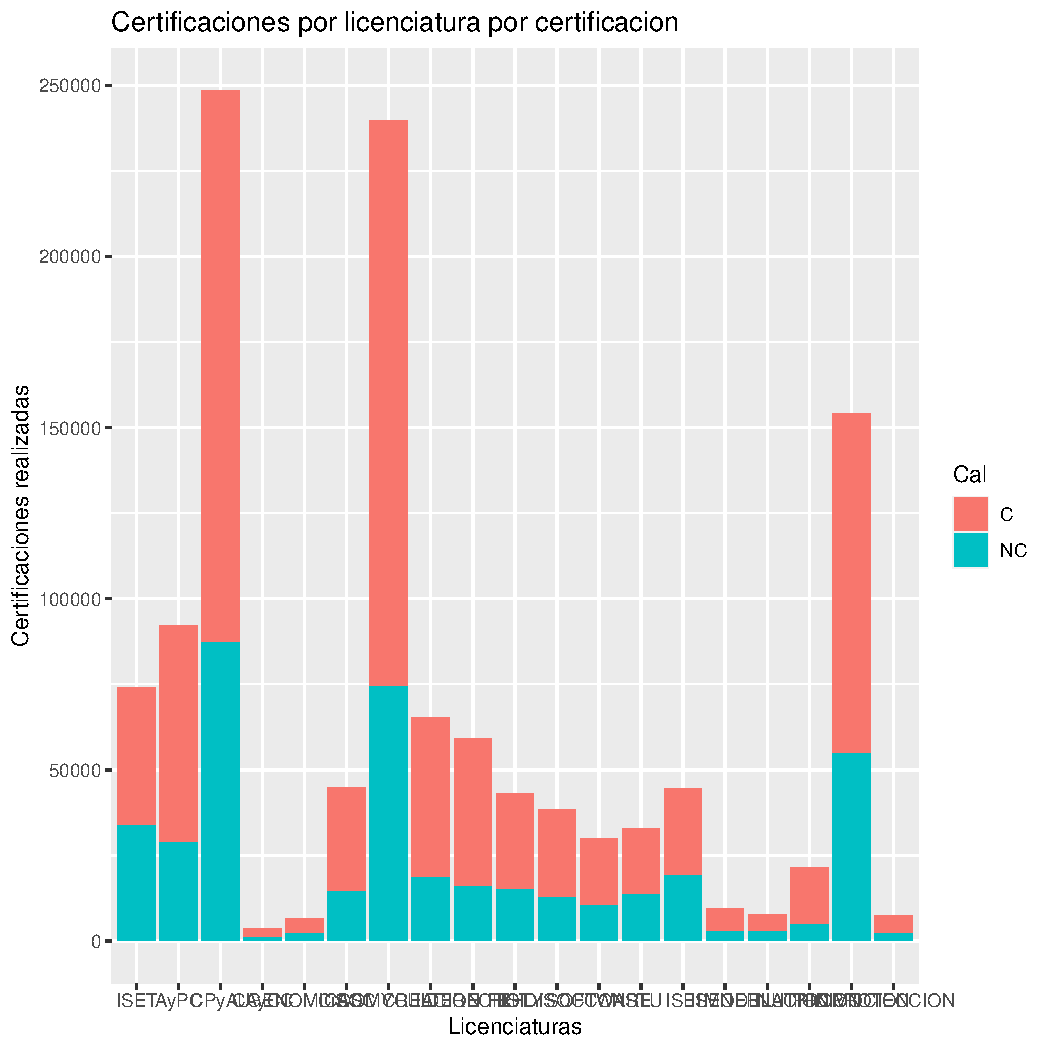
\includegraphics[scale=0.45]{Graficas/ggplotBarplotLicCal.pdf}
\caption{Certificaciones por licenciatura}
\label{Fig.Cert.Lic-Cal}
\end{figure}


\begin{figure}
\centering
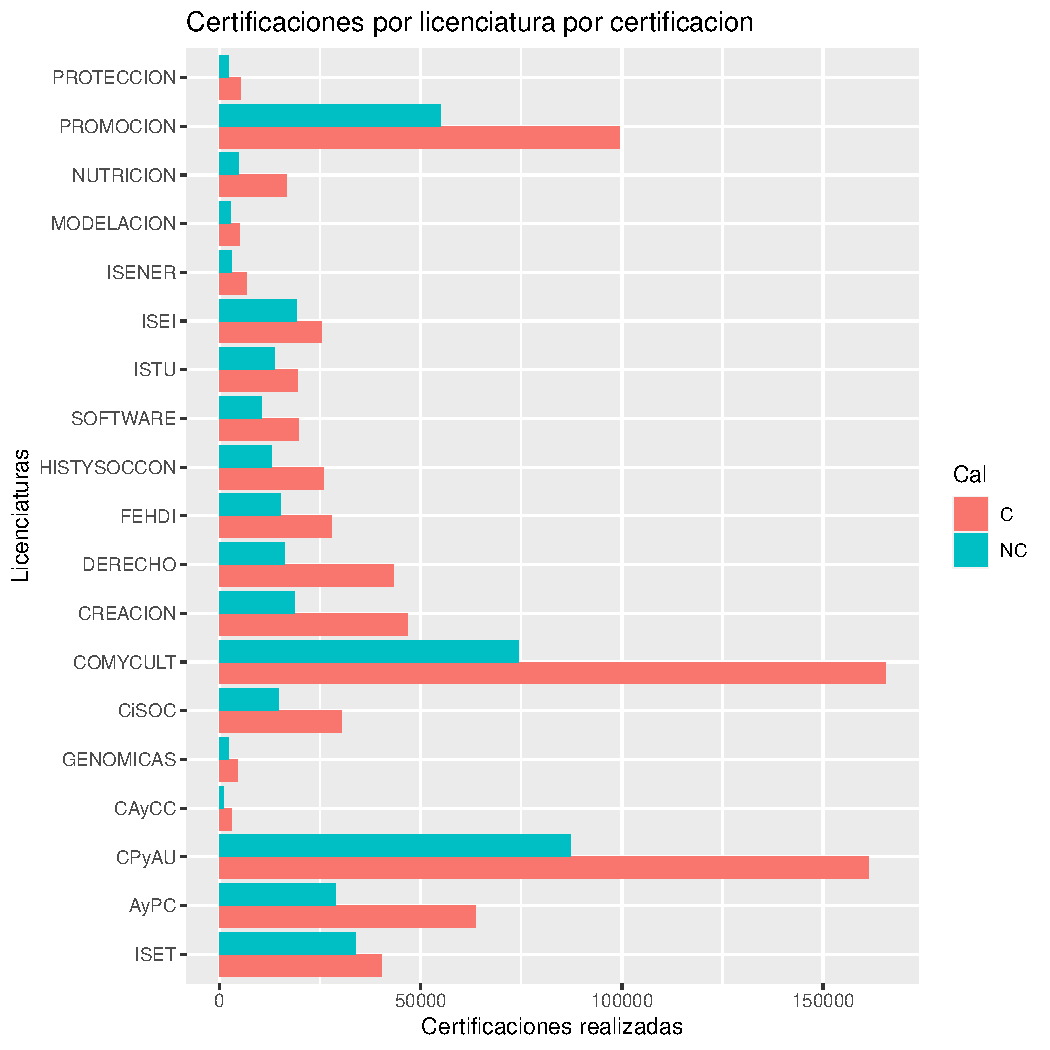
\includegraphics[scale=0.45]{Graficas/ggplotBarplotLicCal2.pdf}
\caption{Certificaciones por licenciatura}
\label{Fig.Cert.Lic-Cal2}
\end{figure}
   


\begin{figure}
\centering
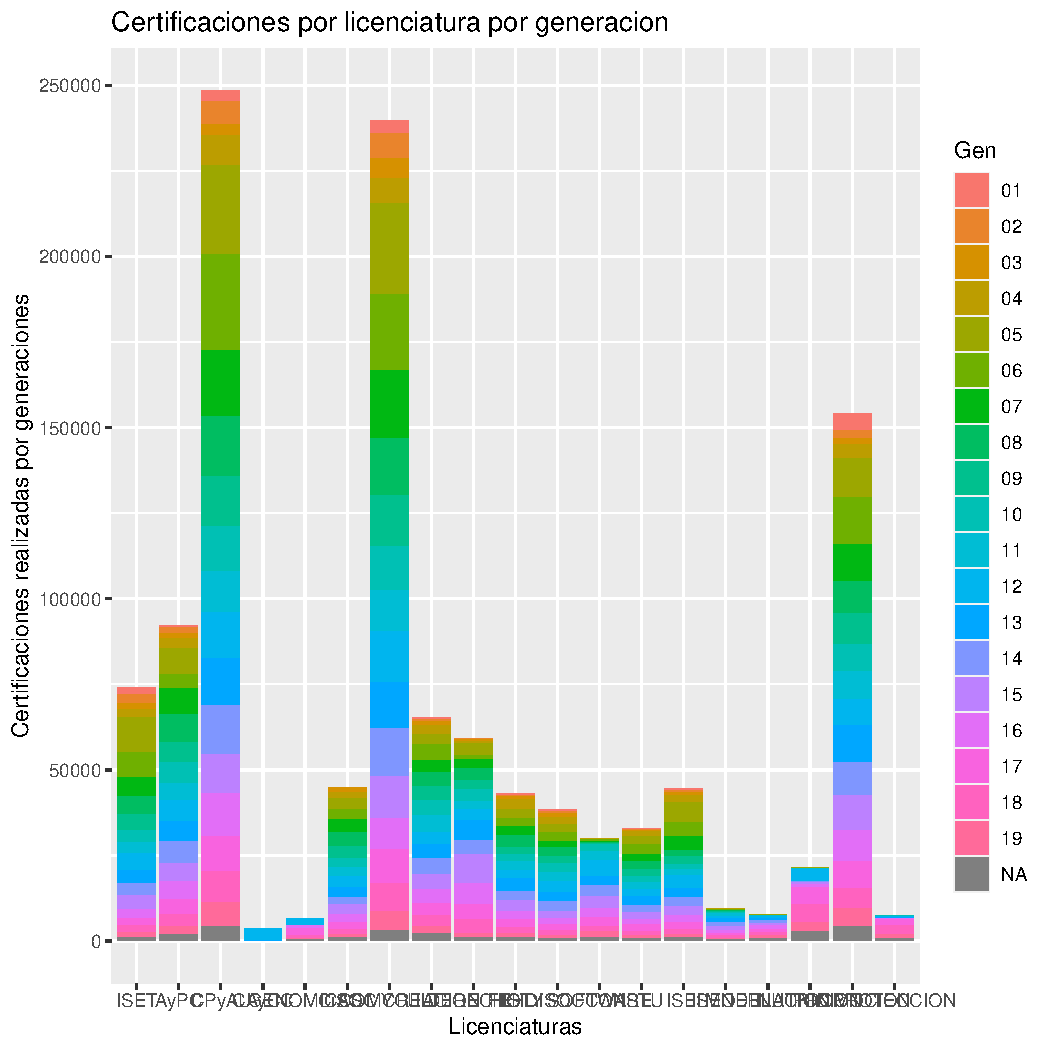
\includegraphics[scale=0.45]{Graficas/ggplotBarplotLicGen.pdf}
\caption{Certificaciones por licenciatura por generacion}
\label{Fig.Cert.Lic-Gen}
\end{figure}

\begin{figure}
\centering
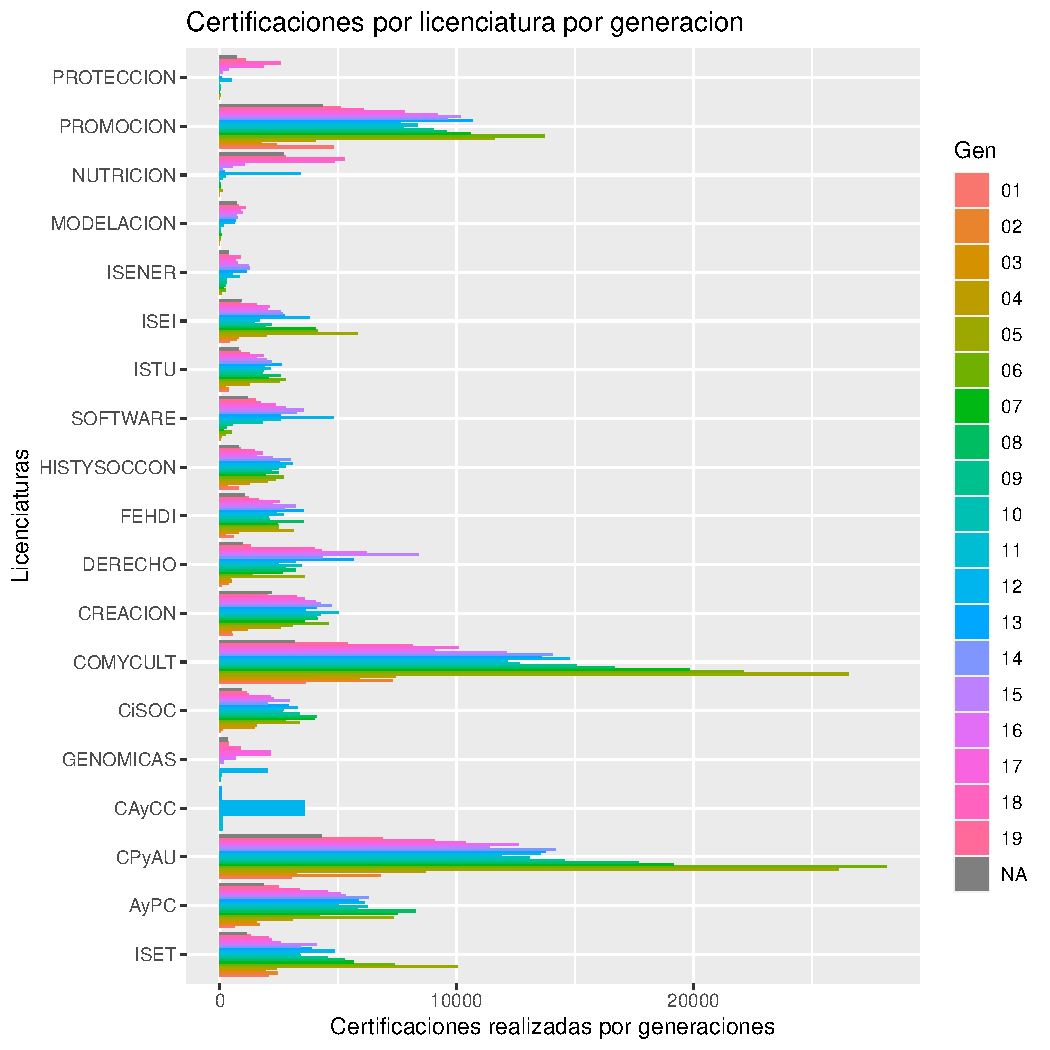
\includegraphics[scale=0.45]{Graficas/ggplotBarplotLicGen2.pdf}
\caption{Certificaciones por licenciatura por generacion}
\label{Fig.Cert.Lic-Gen2}
\end{figure}



\begin{figure}
\centering
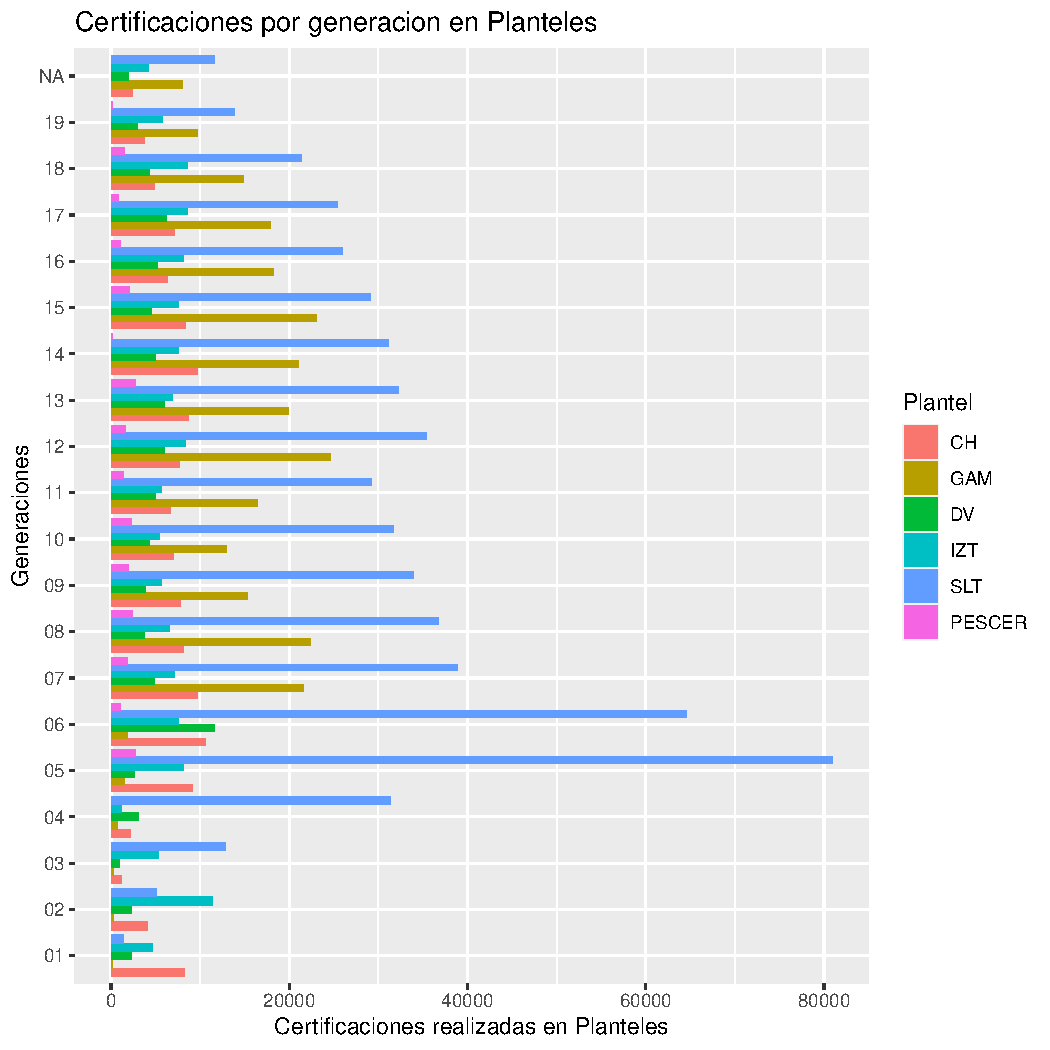
\includegraphics[scale=0.45]{Graficas/ggplotBarplotGenPlantel2.pdf}
\caption{Certificaciones por generaci\'on por planteles}
\label{Fig.Cert.Gen-Plantel2}
\end{figure}

\begin{figure}
\centering
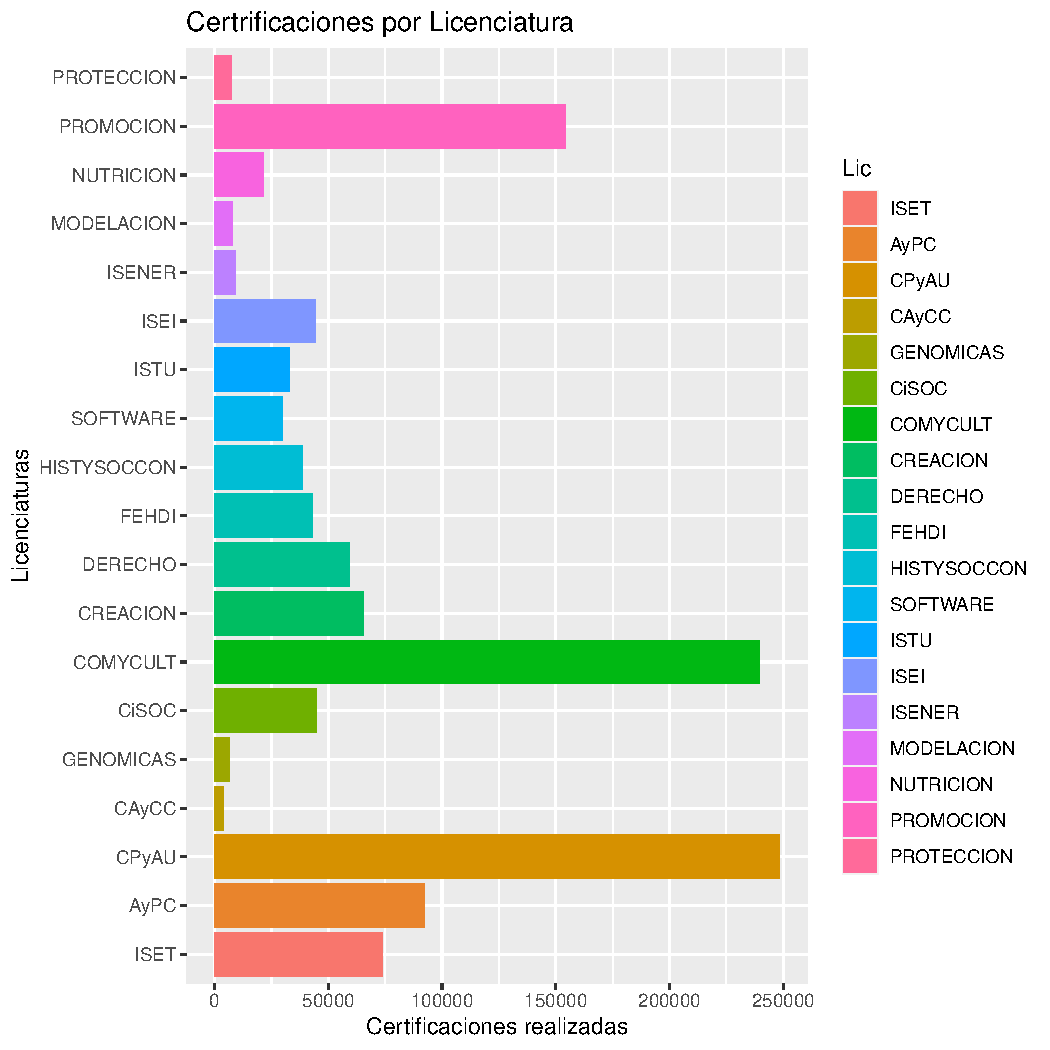
\includegraphics[scale=0.45]{Graficas/ggplotBarplotLic.pdf}
\caption{Certificaciones por licenciatura}
\label{Fig.Cert.Licenciatura}
\end{figure}


\begin{figure}
\centering
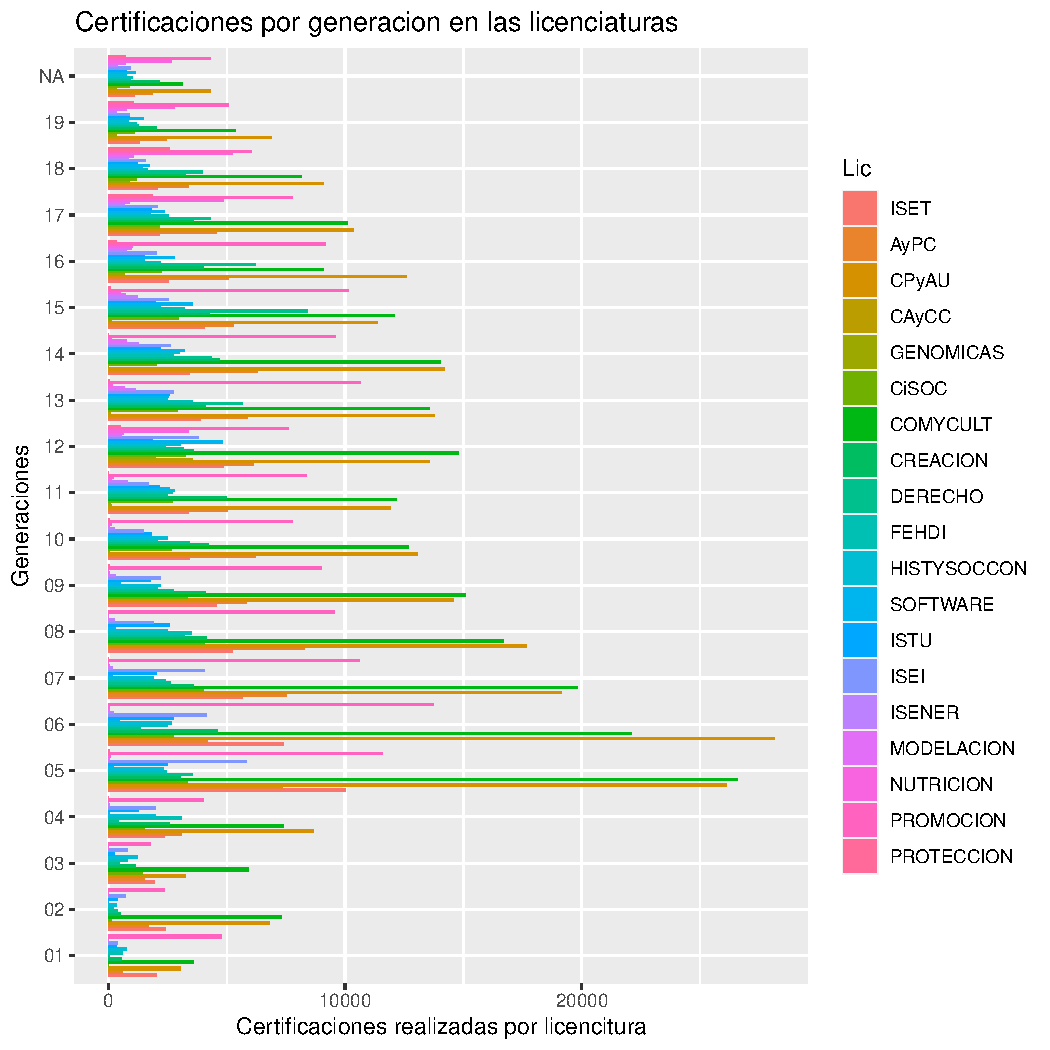
\includegraphics[scale=0.45]{Graficas/ggplotBarplotGenLic2.pdf}
\caption{Certificaciones por generaci\'on por licenciatura}
\label{Fig.Cert.Gen-Lic2}
\end{figure}

\begin{figure}
\centering
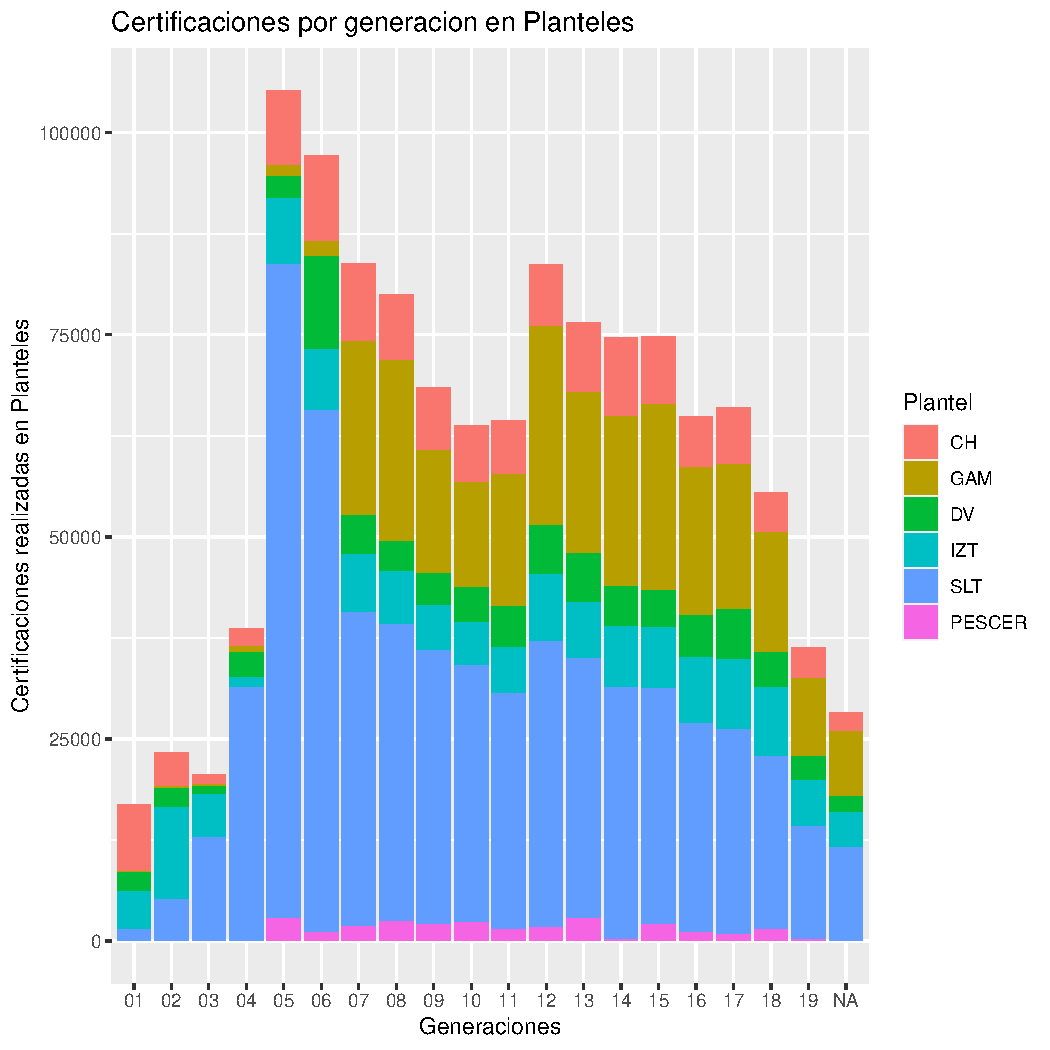
\includegraphics[scale=0.45]{Graficas/ggplotBarplotGenPlantel.pdf}
\caption{Certificaciones por generaci\'on por planteles}
\label{Fig.Cert.Gen-Plantel}
\end{figure}



\begin{figure}
\centering
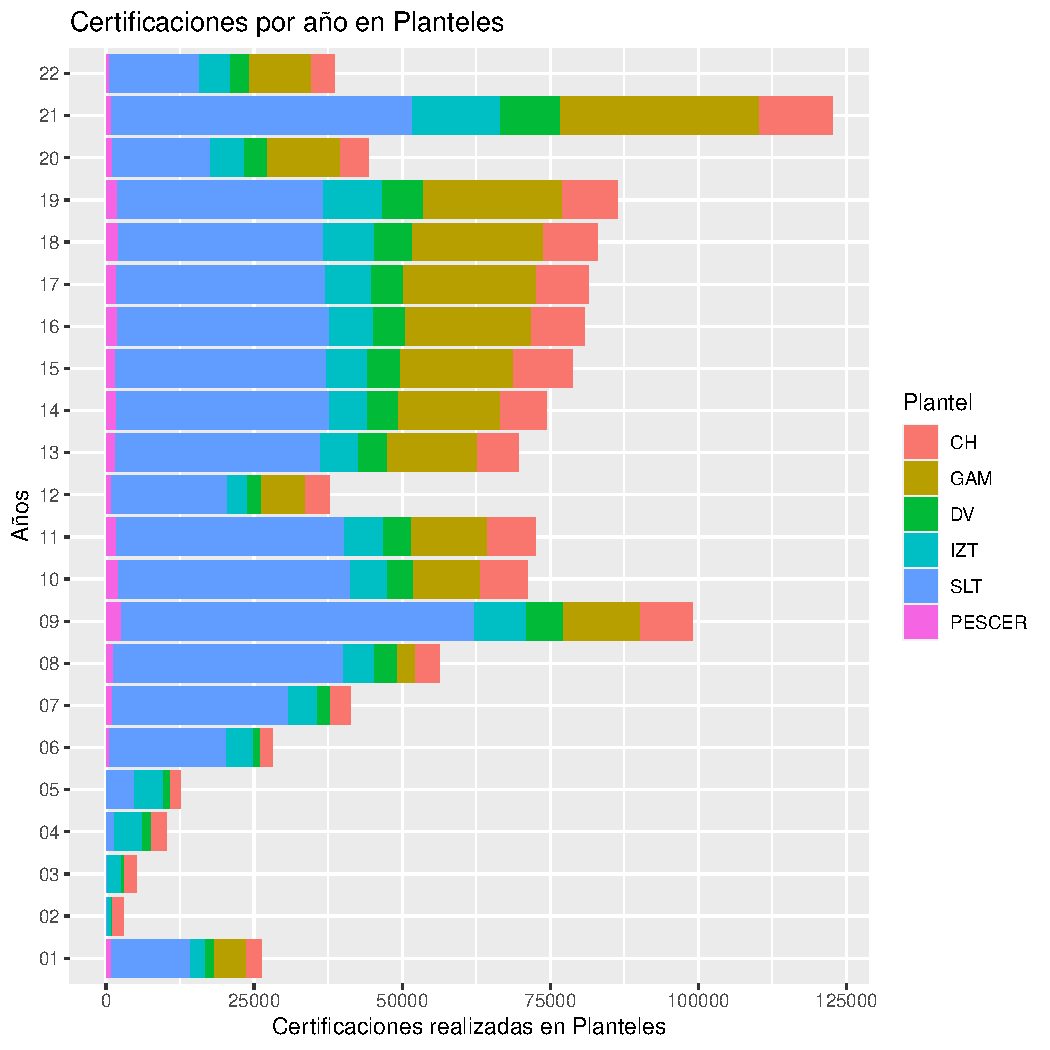
\includegraphics[scale=0.45]{Graficas/ggplotBarplotAnhoPlantel3.pdf}
\caption{Certificaciones por A\~no por plantel}
\label{Fig.Cert.Anho-Plantel3}
\end{figure}
\begin{figure}
\centering
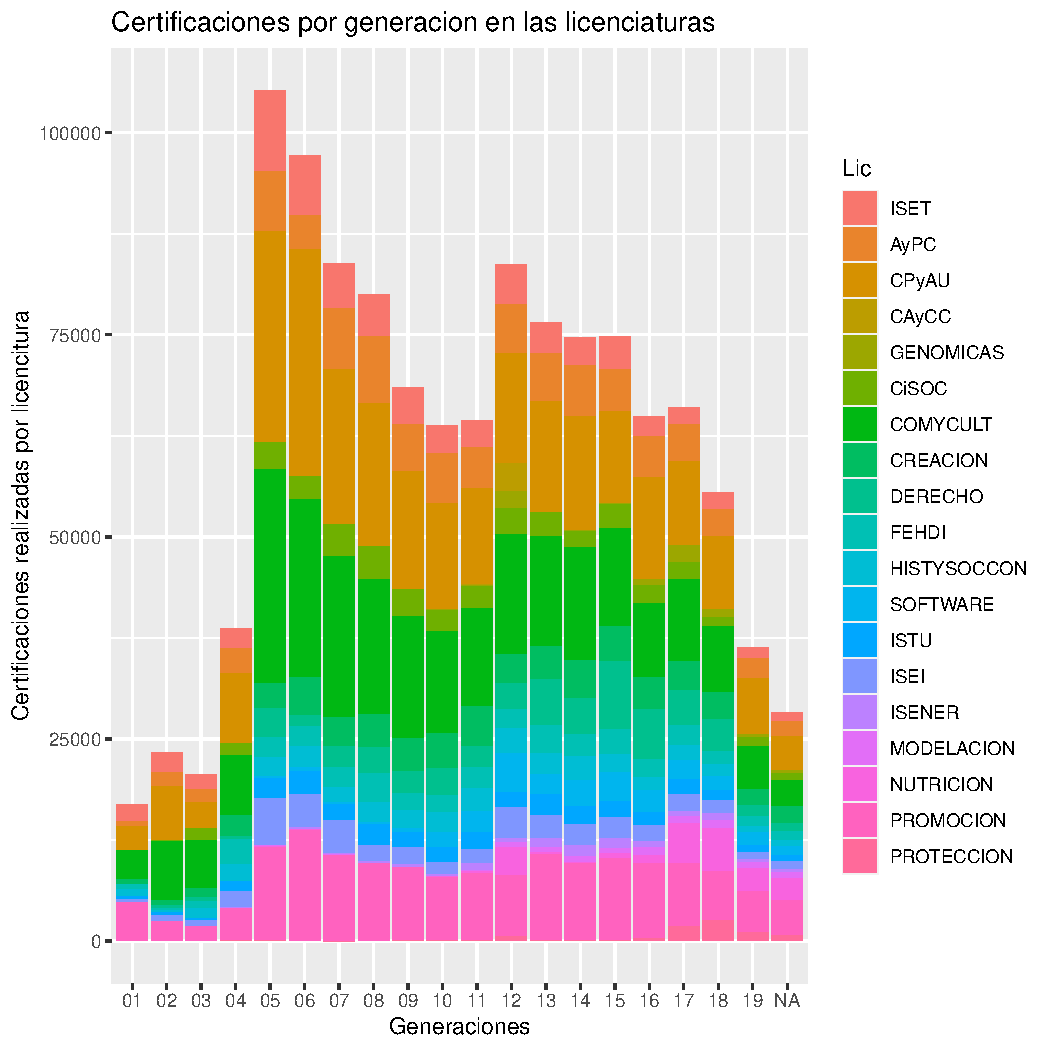
\includegraphics[scale=0.45]{Graficas/ggplotBarplotGenLic.pdf}
\caption{Certificaciones por generaci\'on por licenciatura}
\label{Fig.Cert.Gen-Lic}
\end{figure}


\begin{figure}
\centering
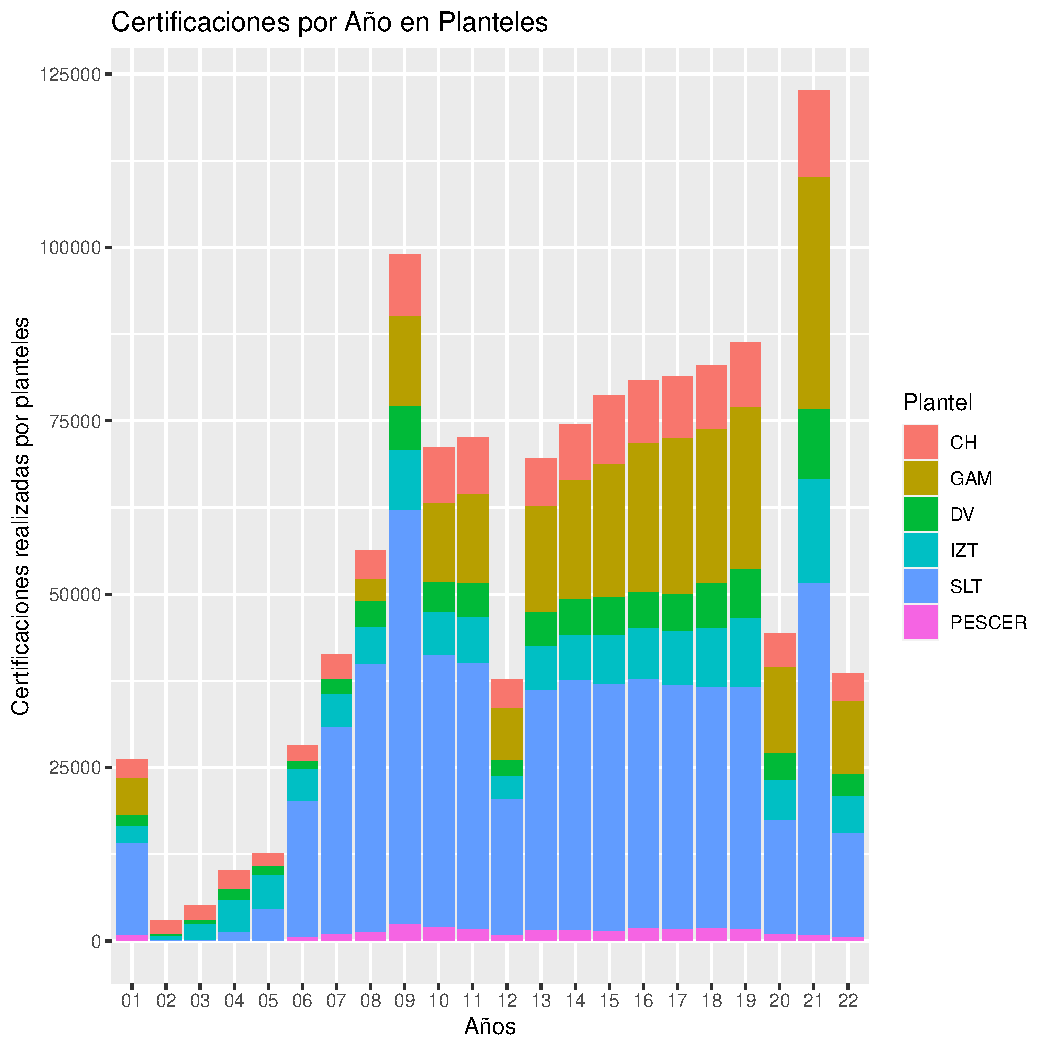
\includegraphics[scale=0.45]{Graficas/ggplotBarplotAnhoPlantel.pdf}
\caption{Certificaciones por A\~no por plantel}
\label{Fig.Cert.Anho-Plantel}
\end{figure}

\begin{figure}
\centering
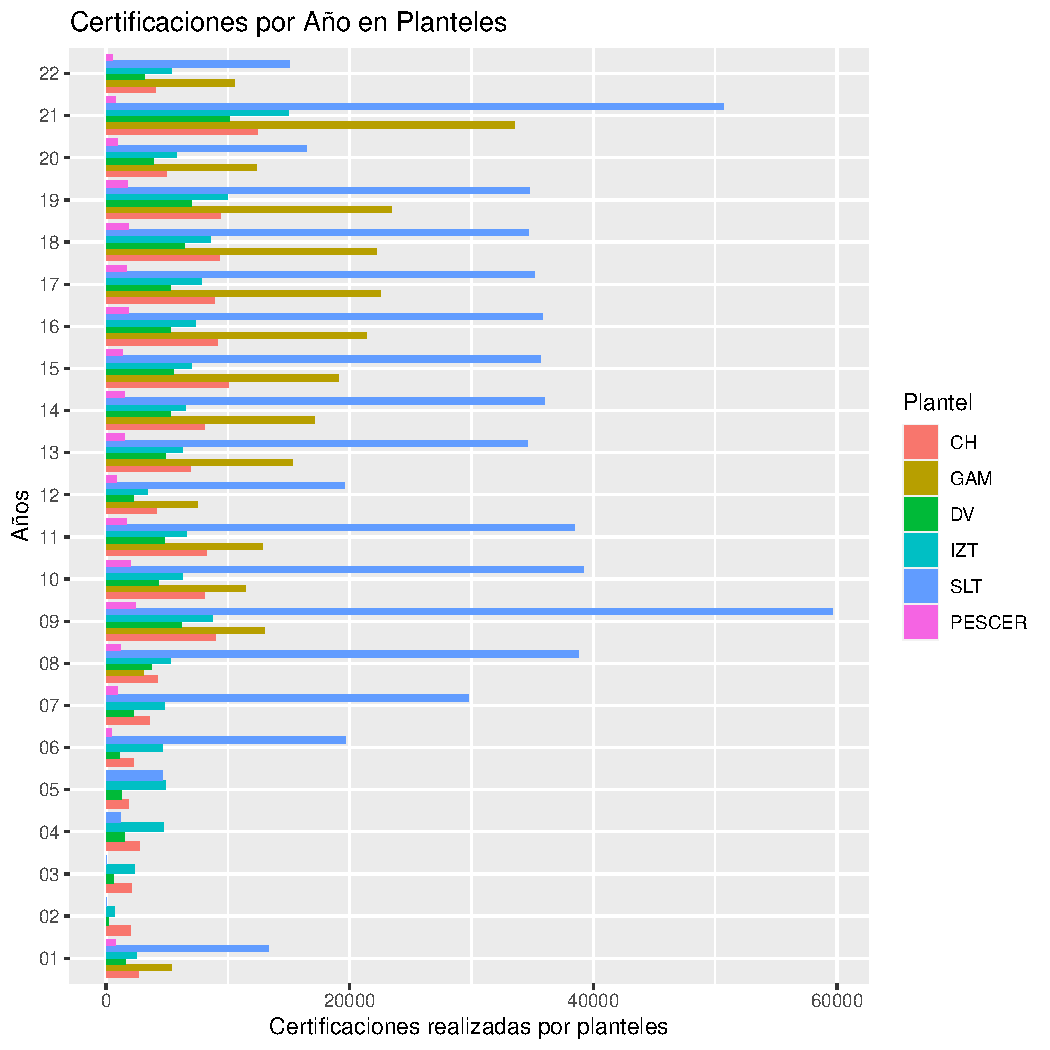
\includegraphics[scale=0.45]{Graficas/ggplotBarplotAnhoPlantel2.pdf}
\caption{Certificaciones por A\~no por plantel}
\label{Fig.Cert.Anho-Plantel2}
\end{figure}


\begin{figure}
\centering
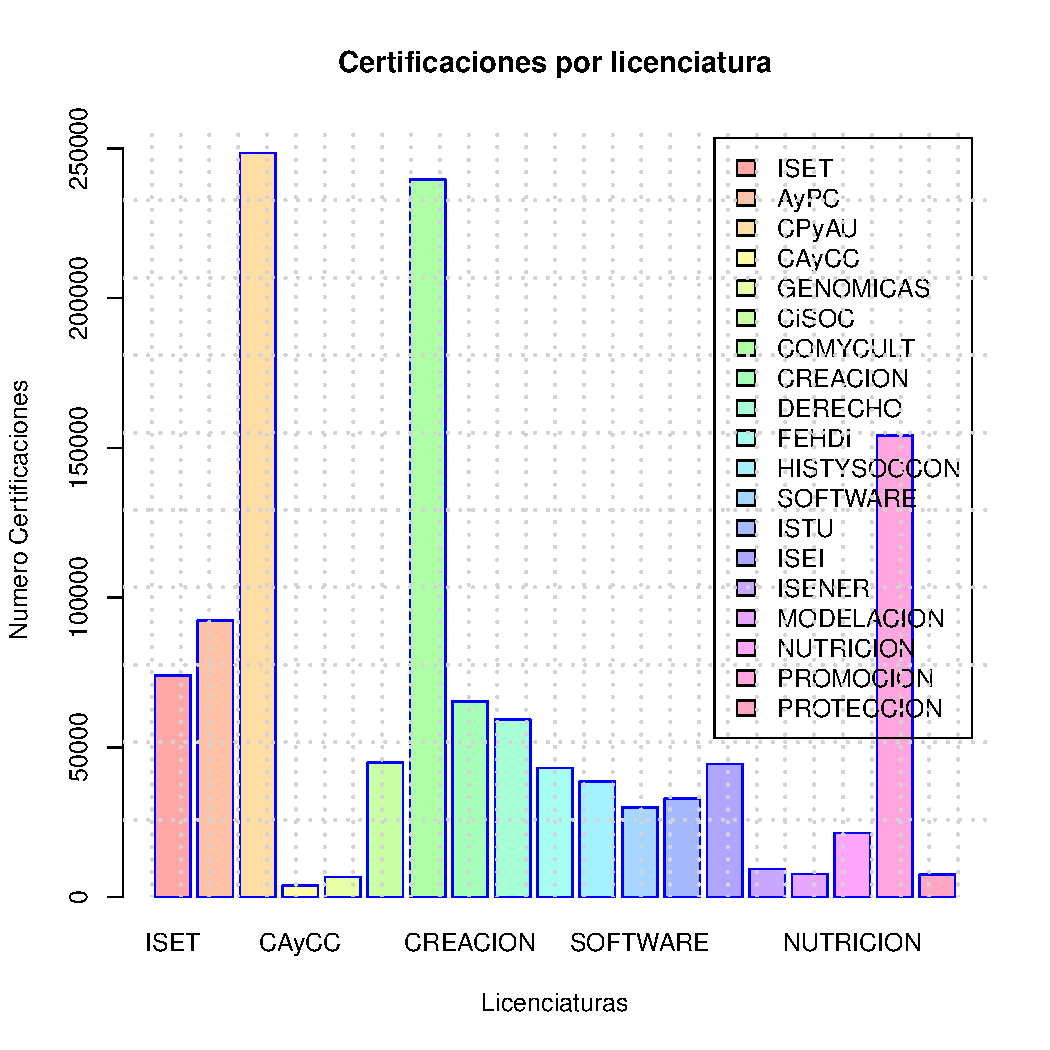
\includegraphics[scale=0.45]{Graficas/BarPlotLic.pdf}
\caption{Certificaciones por licenciatura}
\label{Fig.Cert.Lic}
\end{figure}


\subsection{M'as gr\'aficos}




% << == >>  << == >>  << == >>  << == >>  << == >>  << == >>  << == >>  << == >> 
\begin{thebibliography}{20}
\bibitem{ProyectoEducativo} \textsc{UACM},
\textit{Proyecto Educativo de la UACM},
UACM, M\'exico, DF, 2004.
\bibitem{CircularCertificacion} \textsc{UACM} 
\textit{Circular para regular los procesos y registros de certificaci\'on}, M\'exico, DF, 2007.

\bibitem{Doc3} \textsc{UACM} 
\textit{En qu\'e consiste la certificaci\'on en la UACM}, M\'exico, DF, 20XX.


\end{thebibliography}

\end{document}
